\PassOptionsToPackage{unicode=true}{hyperref} % options for packages loaded elsewhere
\PassOptionsToPackage{hyphens}{url}
%
\documentclass[
  12pt,
  twoside,
  banjiao]{ctexbook}
\usepackage{lmodern}
\usepackage{amssymb,amsmath}
\usepackage{ifxetex,ifluatex}

\usepackage{unicode-math}
\defaultfontfeatures{Scale=MatchLowercase}
\defaultfontfeatures[\rmfamily]{Ligatures=TeX,Scale=1}

% use upquote if available, for straight quotes in verbatim environments
\IfFileExists{upquote.sty}{\usepackage{upquote}}{}
\IfFileExists{microtype.sty}{% use microtype if available
  \usepackage[]{microtype}
  \UseMicrotypeSet[protrusion]{basicmath} % disable protrusion for tt fonts
}{}

\usepackage{xcolor}
\usepackage{xurl} % add URL line breaks if available
\usepackage{bookmark}
\usepackage{hyperref}
\usepackage{placeins}
\hypersetup{
  pdftitle={腹部影像解剖图谱},
  pdfauthor={github},
  pdfborder={0 0 0},
  breaklinks=true,
  bookmarksdepth=4}
\urlstyle{same}  % don't use monospace font for urls
\usepackage{longtable,booktabs}
% Allow footnotes in longtable head/foot
\IfFileExists{footnotehyper.sty}{\usepackage{footnotehyper}}{\usepackage{footnote}}
\makesavenoteenv{longtable}
\usepackage{graphicx,grffile}
\makeatletter
\def\maxwidth{\ifdim\Gin@nat@width>\linewidth\linewidth\else\Gin@nat@width\fi}
\def\maxheight{\ifdim\Gin@nat@height>\textheight\textheight\else\Gin@nat@height\fi}
\makeatother
% Scale images if necessary, so that they will not overflow the page
% margins by default, and it is still possible to overwrite the defaults
% using explicit options in \includegraphics[width, height, ...]{}
\setkeys{Gin}{width=\maxwidth,height=\maxheight,keepaspectratio}

\setlength{\emergencystretch}{3em}  % prevent overfull lines
% Redefines (sub)paragraphs to behave more like sections
\ifx\paragraph\undefined\else
  \let\oldparagraph\paragraph
  \renewcommand{\paragraph}[1]{\oldparagraph{#1}\mbox{}}
\fi
\ifx\subparagraph\undefined\else
  \let\oldsubparagraph\subparagraph
  \renewcommand{\subparagraph}[1]{\oldsubparagraph{#1}\mbox{}}
\fi

% set default figure placement to htbp
\makeatletter
\def\fps@figure{htbp}
\makeatother

\usepackage{framed}
\usepackage{multirow}
\usepackage{ctex}
\usepackage{rotating}
\usepackage{tablefootnote}
\usepackage{caption}
\setCJKmainfont{仓耳明黑}
\setCJKfallbackfamilyfont{\CJKrmdefault}{仓耳明黑}
\setmainfont{仓耳明黑}
\usepackage[a4paper,top=1in, bottom=1in, left=0.8in, right=0.8in]{geometry}
\setlength{\parindent}{2em}
\setlength{\parskip}{0em}

%\newfontfamily\apostrophefont[Ligatures=TeX,Color=FF0000]{Liberation Serif}
\newfontfamily\apostrophefont[Ligatures=TeX]{Liberation Serif}
\XeTeXinterchartokenstate=1
\newXeTeXintercharclass \apostrophe

% Assign the new class to all Latin capital letters
\makeatletter
\@tempcnta=`'
\loop\unless\ifnum\@tempcnta>`'
  \XeTeXcharclass \@tempcnta \apostrophe
  \advance \@tempcnta by 1
\repeat
\makeatother

% Setup font change
\XeTeXinterchartoks 0 \apostrophe   = {\begingroup\apostrophefont}
\XeTeXinterchartoks \apostrophe 0   = {\endgroup}
\XeTeXinterchartoks 4095 \apostrophe = {\begingroup\apostrophefont}
\XeTeXinterchartoks \apostrophe 4095 = {\endgroup}

\renewcommand {\thetable} {\thechapter{}-\arabic{table}}
\renewcommand {\thefigure} {\thechapter{}-\arabic{figure}}

\title{腹部影像解剖图谱}
\author{Github \\ 项目主页:\url{https://github.com/muqiuhan/medical-books}}


\begin{document}
\maketitle

{
\setcounter{tocdepth}{1}
\tableofcontents
\addcontentsline{toc}{chapter}{目录}
}
\newpage

\chapter{细胞和组织的适应、损伤}

\chapterabstract{本章主要介绍组织细胞在病理因素刺激下所出现的适应性改变、变性、异常物质沉积、坏死、凋亡和损伤机制等内容。要求掌握细胞水肿、脂变及透明变性的形态学特征及其对机体的影响,坏死的形态变化和后果,以及各型坏死的形态学及鉴别点;熟悉各种类型萎缩的形态变化及其对机体的影响,凋亡的概念以及与坏死的鉴别;了解各种色素沉着的形态学特征以及组织细胞损伤的机制。}

正常细胞和组织不断受到内外因子的刺激,其物质代谢、形态结构和功能会因此出现相应改变。若刺激在细胞能承受的有限范围内,则表现为适应,属轻度损伤。若刺激时间长强度大,细胞将发生连续反应,表现为适应、损伤,最终导致细胞死亡。严重损伤可以直接导致细胞死亡。正常细胞、适应细胞、损伤细胞和死亡细胞,这四种状态之间界限不清,在形态结构和代谢、功能上的变化是连续的。活体内细胞死亡发生后,机体将给予修复,最大限度地恢复原有细胞和组织的形态结构和功能。

\section{细胞和组织的适应}

在环境发生变化时,机体的细胞和由其构成的组织、器官为了避免损伤,可通过改变自身的代谢、功能和形态结构以适应变化的环境,这种与之协调的过程称为适应。例如当机体突然进入寒冷环境时会全身发抖,这是对环境适应的表现。“发抖”使肌肉活动加强,糖代谢加速,产热增多,以补偿体表丧失的热量。在病理情况下,如高血压病,左心室心肌纤维肥大,收缩力增强,以克服增高的外周阻力,维持血循环正常进行。这些皆属适应性反应。通过适应反应,机体能维持正常的功能,因此适应是正常细胞和损伤细胞的中间状态,在形态学上的改变表现为萎缩、肥大、增生和化生。

\subsection{萎缩}

发育正常的实质细胞、组织或器官体积缩小称为萎缩(atrophy)。通常是由于该器官的实质细胞体积缩小所致,有时也可因细胞数目减少引起,或二者兼有。萎缩有生理性和病理性之分。生理性萎缩与年龄有关,例如青春期胸腺组织萎缩,妇女绝经后卵巢、子宫、乳腺组织萎缩等属于生理性萎缩。病理性萎缩有的表现为全身性,有的表现为局部组织器官萎缩。

\subsubsection{类型}

常见的病理性萎缩按其发生原因分为以下几种类型:

\paragraph{营养不良性萎缩}
有全身性和局部性两种。消化道慢性梗阻(食管癌)和慢性消耗性疾病(如结核病、晚期癌症患者)引起全身性萎缩。这种萎缩首先发生于对生命不太重要的脂肪组织,其次为肌肉、脾、肝、肾等器官,心、脑等生命重要器官萎缩发生最晚,这样的顺序有一定的代偿适应意义。局部营养不良性萎缩见于局部缺血,如动脉粥样硬化使管壁增厚、管腔狭窄、血流减少,引起心、脑、肾等相应器官萎缩。

\paragraph{压迫性萎缩}
常见于尿路结石,阻塞输尿管,引起尿潴留,不断增加的尿液压迫肾组织,使肾实质逐渐萎缩、变薄,最后,整个肾变为充满液体的薄壁巨囊。
这种萎缩除了压迫的直接作用外,还与压迫引起局部血供不良、废用等因素有关。

\paragraph{废用性萎缩}
亦称失用性萎缩。肢体、器官、组织长期不活动,或只担负轻微的活动,功能减退所引起的萎缩。如骨折后肢体长期固定,肌肉、骨组织萎缩。
这种萎缩的发生还与器官停止活动后,向心性或离心性神经刺激减少或消失有关,以致局部血循环和物质代谢降低。

\paragraph{去神经性萎缩}
因运动神经元或轴突损害导致正常神经调节功能丧失,引起效应组织器官营养障碍或血液循环调节异常,并伴有组织功能减低或丧失等综合因素,导致相应部位萎缩。
例如小儿麻痹症(脊髓前角灰质炎)患者由于脊髓前角运动神经细胞死亡,结果受这些细胞支配的肢体肌肉发生麻痹,逐渐萎缩,同时患肢骨小梁变细,钙盐减少,骨质疏松,肢体变得细短。

\paragraph{内分泌性萎缩}
内分泌功能低下时,它所作用的靶器官发生萎缩。如席蒙病(Simmond's
disease)时,由于垂体受到损伤,各种促激素分泌减少,常引起甲状腺、肾上腺、性腺等靶器官萎缩。
老年性萎缩虽然是一种生理现象,也属老年病。
发生机制复杂,与老年期内分泌功能低下、血管硬化、供血不良及运动量减少等众多因素有关。
临床上,某种萎缩可由多种因素所致。

\subsubsection{病理形态}

肉眼观:萎缩的细胞、组织、器官体积变小,重量减轻,颜色变深常呈褐色。
心肌萎缩时冠状动脉在心外膜下呈蛇行弯曲(图\ref{fig1-1}a)。
脑萎缩时,脑回变窄,脑沟变深加宽。镜下观:萎缩的细胞体积变小,或数目减少或两者兼有。
胞浆常深染,核浓缩。心肌萎缩时,其胞浆内可出现棕褐色颗粒,即脂褐素(图\ref{fig1-1}b)。
\begin{figure}[!htbp]
	\centering
	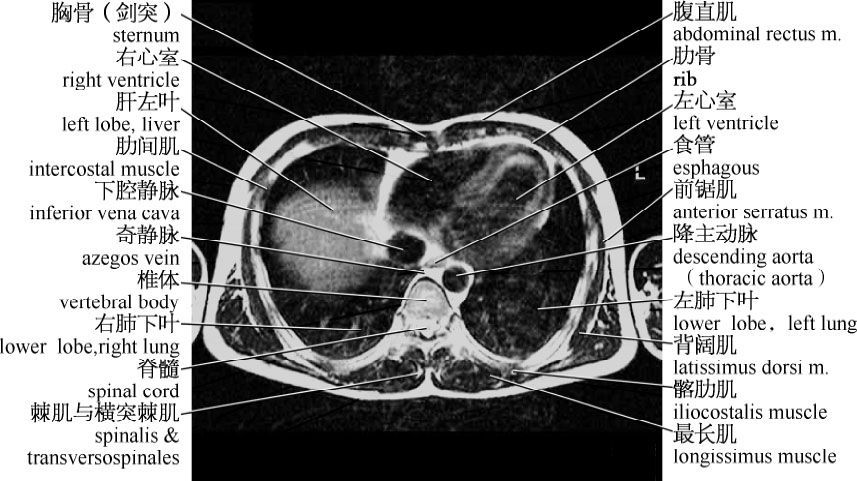
\includegraphics[width=.8\textwidth]{./images/Image00002.jpg}
	\caption{心肌萎缩}
	\label{fig1-1}
\end{figure}
%\FloatBarrier

萎缩的机制尚未完全搞清,蛋白合成少于分解可能为主要原因。

萎缩的器官、组织、细胞功能常降低,但一般是可复性的。原因消除后,萎缩的器官也可恢复正常。如原因持续存在,萎缩的实质细胞最后消失,间质结缔组织和脂肪细胞可以增生,甚至造成器官和组织体积增大,此时称假性肥大。

\subsection{肥大}

由于功能增加、合成代谢旺盛,细胞体积增大,使该器官、组织体积增大,称为肥大(hypertrophy)。肥大多发生于无分裂增殖能力或增殖能力较弱的细胞,如心肌、骨骼肌等。一般可分为生理性肥大和病理性肥大两类。如举重运动员上臂和胸部肌肉的粗壮肥大,妊娠子宫平滑肌细胞肥大属生理性肥大。病理情况下,也可发生肥大。例如高血压病,左心功能负荷加重,心肌纤维体积增大,一侧肾切除后另一侧肾体积增大,皆属代偿性肥大。而成人脑垂体前叶嗜酸细胞瘤分泌过多生长激素,导致的肢端肥大症,则属内分泌性肥大。肥大的细胞除了体积增大外,其内细胞器和微丝明显增多,蛋白合成旺盛。

有时实质细胞萎缩,间质增生也可使该器官、组织体积增大,这种假性肥大与前述的真性肥大有本质的区别。

\subsection{增生}

实质细胞数量增多,使该组织、器官体积增大,称为增生(hyperplasia)。增生可分为生理性和病理性增生两类。妇女在青春期、妊娠期和哺乳期乳腺上皮增生属生理性增生。病理情况下,例如溶血性贫血时骨髓的红细胞系增生,长期缺碘引起甲状腺组织增生,慢性鼻炎黏膜增生肥厚形成息肉等属于病理性增生。由于引起细胞、组织和器官增生与肥大的原因往往十分相似或相同,故两者常同时出现。这种现象见于雌激素过多时引起的子宫内膜增生、乳腺增生,以及老年男性因雄激素代谢障碍导致的前列腺增生。

\subsection{化生}

化生(metaplasia)是指一种已分化成熟的细胞由于适应环境改变而被另一种分化成熟细胞所代替的过程。化生并不是由一种成熟的细胞直接转变为另一种成熟的细胞,而是由该处具有分裂增殖和多向分化能力的幼稚细胞增生,向另一种类型的细胞分化、成熟,也就是所谓的异向分化,是环境因素引起细胞某些基因活化或受到抑制而重新编程表达的结果。化生常发生于同源细胞间,如一种上皮细胞与另一种上皮细胞间。化生是一种可复性病变,原因去除后大多可恢复。常见的化生有:

\subsubsection{鳞状上皮化生}

慢性支气管炎或长期吸烟者,气管及支气管的纤毛上皮转变为鳞状上皮。慢性胆囊炎及胆石症时,胆囊黏膜上皮发生鳞状上皮化生。慢性宫颈炎、子宫内膜炎时,黏膜上皮发生鳞状化生,在妇产科极为常见(图\ref{fig1-2})。肾盂结石时,肾盂黏膜的移行上皮也可转变为鳞状上皮。
\begin{figure}[!htbp]
	\centering
	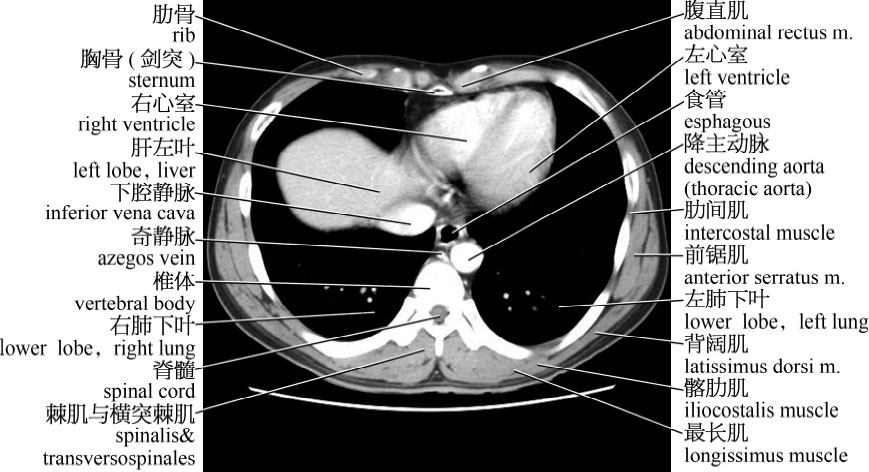
\includegraphics{./images/Image00003.jpg}
	\caption{子宫内膜鳞状上皮化生(HE染色,高倍) \\ {\small 子宫内膜的纤毛柱状上皮化生为鳞状上皮}}
	\label{fig1-2}
\end{figure}
%\FloatBarrier

\begin{framed}
	{案例1-1}

	{【病例摘要】}

	患者,男,55岁,因醉酒后呕吐、误吸,呛咳、呼吸困难入院。全麻下行支气管镜检查,从右主支气管中取出少量未消化米粒和菜叶,症状缓解;术中发现支气管黏膜充血、粗糙,征得家属同意后,夹取2块黏膜组织送病理检查。患者有吸烟史30年,反复咳嗽、咳痰史10年,否认其他病史。病理报告为“送检组织为少量鳞状上皮及其下疏松结缔组织、腺体,伴小血管充血和淋巴细胞、浆细胞浸润。符合慢性支气管炎。”

	{【问题】}

	(1)该患者支气管黏膜出现鳞状上皮,此属何种病理现象?

	(2)试分析病变形成机制和意义。
\end{framed}

\subsubsection{肠上皮化生}

慢性胃炎时,部分胃黏膜上皮转变为含有杯状细胞、潘氏细胞及具有纹状缘的吸收上皮,与小肠黏膜上皮相似;或在柱状上皮中,间有杯状细胞,与大肠黏膜上皮相似,均称为肠上皮化生(简称肠化)。类似的化生也常发生于腺体,由一种腺上皮转变为另一种腺上皮,故又称腺性化生。

\subsubsection{结缔组织和支持组织化生}

纤维组织化生为脂肪组织或肌细胞,成纤维细胞转变为骨母细胞或软骨母细胞,分别化生为骨或软骨(图\ref{fig1-3})。
\begin{figure}[!htbp]
	\centering
	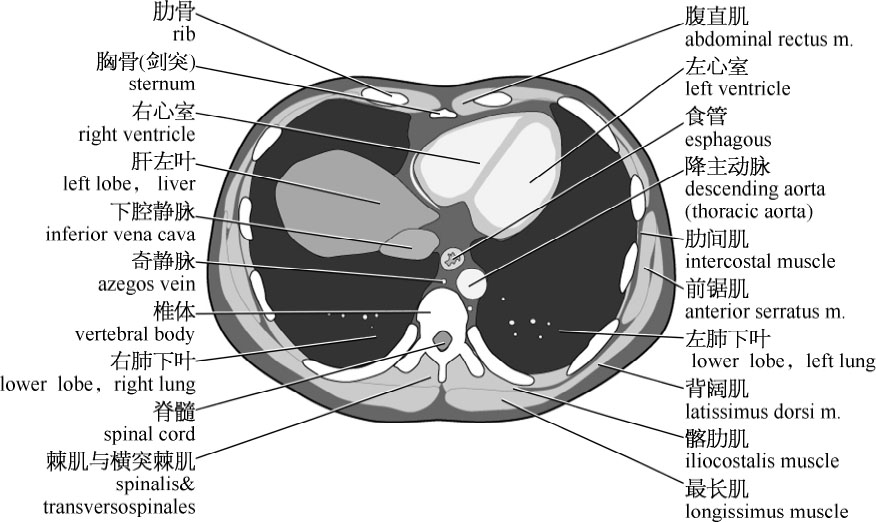
\includegraphics{./images/Image00004.jpg}
	\caption{心瓣膜软骨化生(HE染色,高倍) \\ {\small 心瓣膜结缔组织出现软骨化生}}
	\label{fig1-3}
\end{figure}
%\FloatBarrier

\begin{center}
	\textbf{知识链接}
\end{center}
\chapterabstract{上皮间质转分化(epithelial-mesenchymal
transition)为近年研究热点,其实也是一种化生现象。它是指上皮细胞在某些因素刺激下,逐渐失去上皮细胞表型(如E钙黏蛋白、细胞骨架蛋白等的表达)而呈现间质细胞表型(如波形蛋白、平滑肌肌动蛋白、纤维连接蛋白等的表达)。该现象可见于多种生理病理过程,如胚胎发育、组织重塑、肿瘤侵袭转移、慢性炎症和器官纤维化等。}

化生是机体对环境中不良因子发生防御反应的一种形式,对机体是有利的,但也有其局限性和不完善性。例如支气管黏膜鳞状化生后,失去纤毛,削弱了黏膜的自净能力。在化生、增生的基础上,还可能发展为肿瘤。例如支气管鳞状上皮化生和胃黏膜肠上皮化生,分别与肺鳞状细胞癌和胃腺癌的发生有一定的关系。

综上所述,组织细胞为了适应内外环境的变化,可出现萎缩、肥大、增生和化生等形态学改变(图\ref{fig1-4})。若刺激因素使发育正常的组织或器官内实质细胞体积缩小或数目减少即称为萎缩;实质细胞体积增大,即称为肥大;实质细胞数量增多,即称为增生;已分化成熟的细胞被另一种分化成熟细胞所代替即称为化生。

\begin{figure}[!htbp]
	\centering
	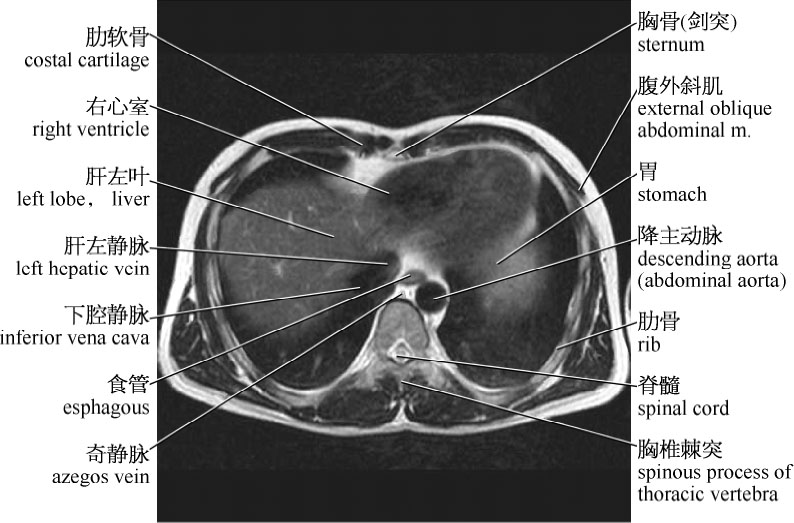
\includegraphics{./images/Image00005.jpg}
	\caption{四种适应性改变示意图}
	\label{fig1-4}
\end{figure}
%\FloatBarrier

\section{细胞和组织的损伤}

当损伤因素超出机体的适应能力,则引起细胞和组织的损伤。在一定程度内这种损伤为可复性,形态上表现为变性和物质异常沉积。重度损伤则引起细胞和组织的死亡。

\subsection{细胞和组织损伤的原因与发生机制}

\subsubsection{缺氧}

缺氧是引起组织细胞损伤常见而重要的原因。缺氧常见于:各种原因造成动脉供血不足或静脉回流障碍,或由于呼吸、循环障碍使血氧含量不足,也可见于严重贫血或中毒(如CO中毒)使红细胞携氧能力降低等情况。缺氧首先影响细胞的需氧呼吸,即线粒体的氧化磷酸化功能,使ATP产生减少或停止,导致细胞膜的钠泵功能障碍,Na{+}
及水在细胞内集聚,K{+}
从细胞外溢,造成急性细胞肿胀。缺氧也使无氧酵解过程增强,通过糖原分解产生ATP,以维持细胞的能量,但在无氧酵解的过程中细胞内乳酸、酮体、氨基酸和无机酸等氧化不全的代谢产物大量积聚,使pH下降。随之粗面内质网核蛋白体脱失、裂解,并出现线粒体肿胀,内质网扩张等一系列超微结构改变。以上改变是可复性的,随缺氧的恢复而恢复正常。如缺氧持续存在,ATP供应耗竭,细胞酶系统广泛损伤,细胞膜功能严重受损,细胞外Ca{2+}
不断进入细胞内,甚至进入线粒体内,使其基质中出现无定形的富于钙的致密区,线粒体发生不可复性改变,以至参与代谢的某些酶活性受抑,并使蛋白变性,细胞死亡。细胞内pH进一步下降将导致溶酶体膜的损伤,其内多种酶进入细胞浆内并被激活,其中酸性水解酶可引起细胞自溶死亡。

不同组织细胞对缺氧的耐受程度不同。结缔组织对缺氧耐受时间最长,而神经细胞对氧极为敏感,缺氧长于5~10分钟,细胞则发生不可复性损伤。

\subsubsection{物理因子}

物理因子包括机械性、高温、低温、电流、放射线等刺激因子。机械性损伤能使细胞组织破裂;高温使细胞内蛋白质(包括酶)变性,低温可使血管收缩引起组织缺血性损伤,或造成局部血流停滞、凝血,甚至细胞内水分形成冰晶而损伤细胞;电流通过组织时引起高温灼伤局部组织;放射线作用于机体能直接或间接造成大分子损伤,使水分被激发电离,产生大量具有强毒力的自由基,损伤组织细胞。物理因子引起损伤的严重程度主要决定于该物理因子的作用性质、强度和持续时间的长短,而很少和机体的反应性有关。

\subsubsection{化学因子}

许多化学物质进入人体,在组织细胞内发生化学反应,可破坏正常的生理功能。化学物质造成组织损伤前提是它们必须能经口、呼吸道、皮肤或黏膜进入体内才能引起中毒。化学因子引起损伤的机制是多方面的:①直接损伤:如强酸、强碱可直接灼伤皮肤或黏膜,引起局部炎症或坏死;②抑制酶的活性:如有机磷农药能抑制胆碱酯酶的活性,引起损伤。氯化汞和体内的巯基结合,从而使许多酶蛋白失去活性或破坏膜蛋白结构;③通过代谢形成毒性代谢产物而发挥作用:例如,四氯化碳经肝细胞滑面内质网所含的细胞色素P-450混合功能氧化酶类的作用,裂解生成毒性物质CCl{3}
和Cl自由基,后者可引起肝细胞发生脂肪变性和坏死。

自由基(free
radical)又称游离基,是指一类含有未配对电子的化学基团,如H{+} 、OH{-}
、HOO、O{2-}
,其化学活性高而不稳定,它与细胞内各种有机或无机化合物,如脂质、蛋白质、核酸等,发生过氧化、交联或断裂,从而造成细胞的损伤。但在正常人体内,自由基在细胞外液中的浓度极低,不构成对细胞的威胁,而在吞噬细胞杀灭病原生物或抗肿瘤细胞过程中自由基却起重要防御作用。但是如果体内生成过多,或清除障碍,如在上述的化学性、放射性、炎症损伤过程中,或随着年龄的增长,机体抗氧化活性递减,逐级降低对自由基的防御能力,均可引起组织细胞损伤或机体衰老。自由基可在正常新陈代谢中产生,是普遍存在于生物系统的代谢中间产物,种类多,数量大,活性高。

\subsubsection{生物性因子}

生物性因子是引起细胞损伤最常见的原因,包括病毒、细菌、立克氏体、真菌、寄生虫等引起的各种感染。其作用机制有下列几方面:①直接作用损伤细胞和组织:病毒寄生于细胞内干扰细胞的代谢活动,使细胞变性坏死。②通过内外毒素的作用或产生的毒性代谢产物:如白喉外毒素自由基能抑制细胞的氧化过程和蛋白质的合成。溶血性链球菌产生的透明质酸酶和链激酶引起间质损伤。③生物因子具有抗原性,能引起变态反应:肝炎病毒有嗜肝细胞的特性并产生病毒蛋白,后者可通过变态反应引起肝细胞损伤。

\subsubsection{免疫反应}

免疫反应是机体的正常防御功能,通过免疫反应排斥异己物质,以维持内环境的稳定。但这种反应结果并非均对机体有利,例如病毒性肝炎,在机体T细胞致敏清除肝炎病毒的过程中也造成肝细胞的损伤;在某些情况下对病原生物产生的抗体与体内组织抗原发生交叉反应,形成抗原抗体复合物沉积于组织,引起损伤,如风湿性心肌炎,急性肾小球肾炎,通过变态反应对自身组织抗原发生反应,引起组织细胞的损伤;甚至针对自身组织发生自身免疫反应,如红斑性狼疮,类风湿关节炎等。

\subsubsection{其他}

遗传缺陷、营养失衡、内分泌异常、衰老、心理和社会因素等也能导致组织细胞的损伤。

综上所述,引起组织细胞损伤的因子很多,它们主要通过以下几个途径造成细胞损伤(图\ref{fig1-5}):①ATP耗竭,细胞需要能量的生理活动受阻;②细胞膜完整性破坏、渗透性缺陷,导致细胞内容物流失或物质交换和电生理活动异常;③细胞内钙离子浓度升高,多种酶被激活,使ATP耗竭或细胞结构的破坏;④自由基产生增多;⑤其他代谢活动异常等。一种因子可通过多种途径损伤细胞,几种因子亦可共用一条途径使细胞受累。
\begin{figure}[!htbp]
	\centering
	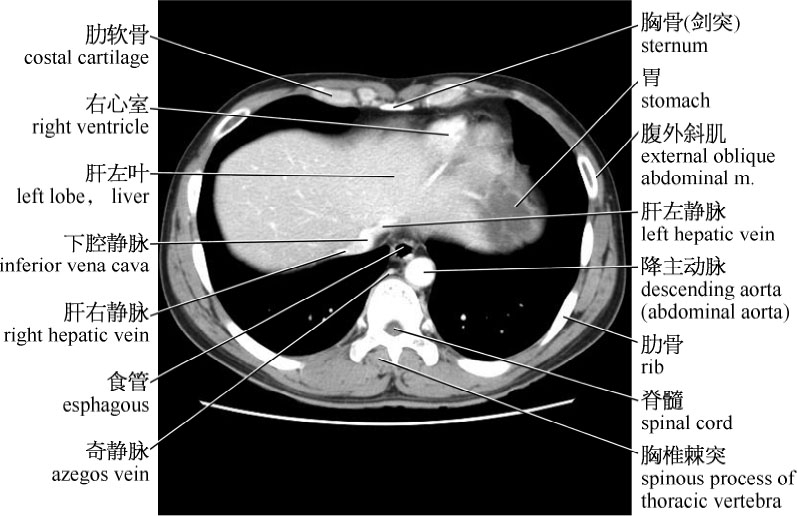
\includegraphics{./images/Image00006.jpg}
	\caption{组织细胞损伤机制示意图}
	\label{fig1-5}
\end{figure}
%\FloatBarrier 

\subsection{细胞和组织损伤的形态学变化}

组织细胞损伤有轻重之别,损伤因子强度弱、作用时间短,细胞的损伤可恢复,即为可逆性损伤;若损伤因子持续刺激和过于剧烈,细胞将会死亡,则表现为不可逆性损伤。

\subsubsection{可逆性损伤}

可逆性损伤(reversible
injury),旧称变性(degeneration),是指新陈代谢障碍时,细胞或细胞间质内出现一些异常物质或正常物质异常蓄积。变性的组织细胞功能下降,但通常为可复性,严重者可发展为坏死。变性的种类繁多,下面介绍比较常见的几种变性。

\paragraph{细胞水肿}
细胞水肿(cellular edema)或称水变性(hydropic
degeneration)即细胞内水钠积聚过多,引起细胞体积肿大,胞浆疏松、透明淡染。常见于缺氧、感染、中毒时的心、肝、肾等脏器的实质细胞。

病理上,轻度的细胞水肿,胞浆内出现许多细小的伊红染颗粒,此乃水肿时肿大的线粒体和扩张的内质网,这种变化致相应器官肉眼观时体积轻度增大,包膜紧张,颜色较正常淡,显得混浊而无光泽,在电镜技术问世之前称之为颗粒变性(granular
degeneration)或混浊肿胀,此名词现已弃用。随细胞内水钠积聚增多,细胞水肿进一步发展,线粒体和内质网高度扩张,囊泡变,此时镜下观:胞浆透明、空泡状,故又有空泡变性或水样变性之称(图\ref{fig1-6})。病毒性肝炎和四氯化碳中毒时,肝细胞水肿,严重者细胞肿大如圆球状,特称为气球样变(图\ref{fig1-7})。
\begin{figure}[!htbp]
	\centering
	\begin{minipage}[b]{0.45\textwidth}
		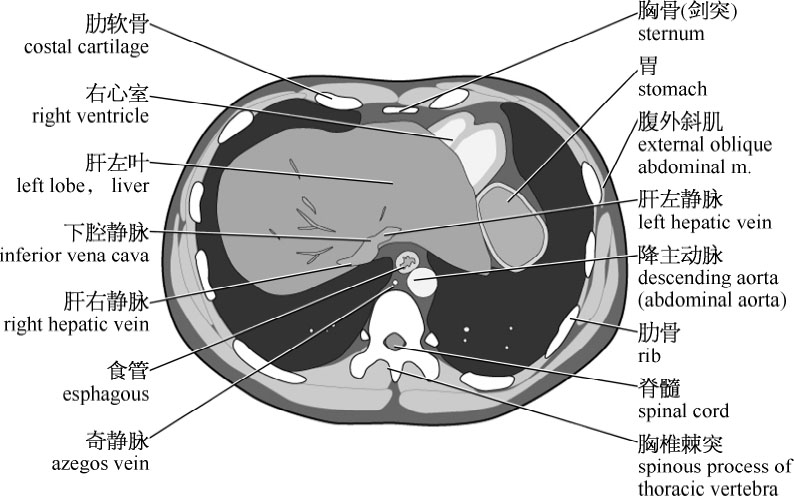
\includegraphics{./images/Image00007.jpg}
		\caption{肾小管上皮细胞水肿(HE染色,高倍) \\ {\small 细胞体积增大,胞浆内出现红染的颗粒状物}}
		\label{fig1-6}
	\end{minipage}
	%	\end{figure} 
	%\FloatBarrier
	%\begin{figure}[!htbp]
	%    \centering
	\hspace{0.04\textwidth}%
	\begin{minipage}[b]{0.45\textwidth}
		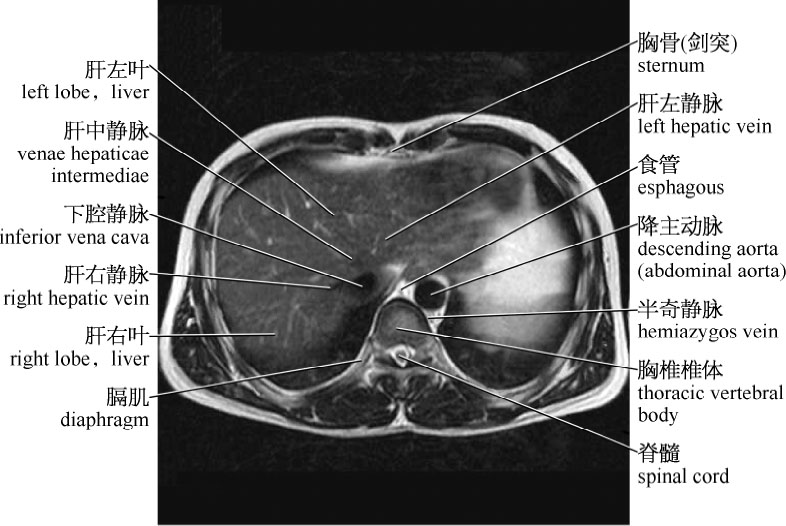
\includegraphics{./images/Image00008.jpg}
		\caption{肝细胞水肿(HE染色,中倍) \\ {\small 肝细胞明显肿胀,细胞浆疏松}}
		\label{fig1-7}
	\end{minipage}
\end{figure}
%\FloatBarrier

引起细胞水肿的原因很多,在急性感染、缺氧、中毒等有害因素的作用下,线粒体产能机制受损,ATP生成减少,使细胞膜的钠泵功能障碍,导致细胞内水、钠增加,细胞水肿。或由于细胞膜直接受损,通透性增高所致。

细胞水肿是一种轻度或中度损伤的表现,在原因消除后,仍可恢复正常。若病因持续存在,水肿细胞的胞浆内可出现脂滴空泡。严重水肿可引起细胞坏死。

\paragraph{脂肪变性}
除脂肪细胞外,其他细胞胞浆内出现脂滴或脂滴明显增多称为脂肪变性(fatty
degeneration),简称脂变。脂变常发生于心、肝、肾等代谢旺盛或耗氧较多的器官。脂变中的脂滴,主要成分为中性脂肪,也可有磷脂及胆固醇等成分,在常规石蜡包埋的切片中,中性脂肪被制片过程中所使用的乙醇、二甲苯等脂溶剂溶解,所以HE染色的切片,光镜下细胞中的脂滴呈空泡状。在冰冻切片苏丹Ⅲ染色时显示脂肪滴为橘红色,锇酸染色时呈黑色。

(1)肝脂肪变性:由于肝脏在脂肪代谢中起重要作用,故肝脂变最多见,且常较严重。肉眼观:轻度脂变时肝脏无明显改变,脂变广泛时肝脏均匀性肿大,包膜紧张,边缘钝,色淡黄,切面有油腻感,苏丹Ⅲ染色后变成红色(图\ref{fig1-8}a)。镜下观:HE染色切片可见早期脂变表现为核周围出现小的脂肪空泡,以后渐增大,散布于胞浆中,严重时融合成一个大空泡,将核推挤到包膜下,状似脂肪细胞(图\ref{fig1-8}b)。脂变在肝小叶内的分布与病因有一定的关系。如肝淤血时,小叶中央区淤血明显,缺氧较重,脂变首先发生于此处。长期淤血,小叶周边区肝细胞也因缺氧而发生脂变,而小叶中央区的肝细胞大多已萎缩或消失。磷中毒时,脂变主要发生在小叶周边区,可能与该区肝细胞代谢较为活跃,对磷中毒更为敏感所致。此外,小叶周边的肝细胞接触到的毒物浓度较高也使此处的肝细胞易受损伤。
\begin{figure}[!htbp]
	\centering
	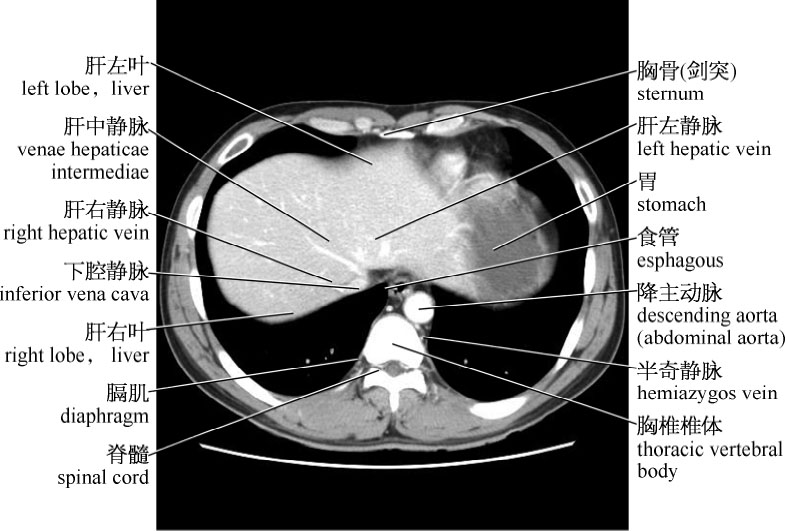
\includegraphics{./images/Image00009.jpg}
	\caption{肝脂肪变性}
	\label{fig1-8}
\end{figure}
%\FloatBarrier 



肝脂变是可复性损伤,病因消除后,脂变细胞可恢复正常,一般无明显的临床表现。重度弥漫性肝脂变称为脂肪肝,体检时肝可在右季肋下触及,常规B超可进行诊断。病变持续发展,肝细胞逐渐坏死,纤维组织增生,可发展为肝硬化。

(2)心肌脂肪变性:多见于贫血。肉眼观:轻度脂变一般无明显异常,但在严重贫血时,常在心内膜下,尤其是左心室乳头肌处出现红黄相间的条纹,如虎皮斑纹,称为“虎斑心”。这是由于心肌内血管分布不均,心肌缺氧轻重程度不一所致,血管末梢分布区心肌缺氧较重,脂变明显而呈黄色,缺氧较轻部位脂变较轻,心肌呈红色。镜下观:脂肪空泡常较细小,呈串珠状排列。有时心外膜增生的脂肪组织可沿间质深入心肌细胞间,称为心肌脂肪浸润(图\ref{fig1-9})。
\begin{figure}[!htbp]
	\centering
	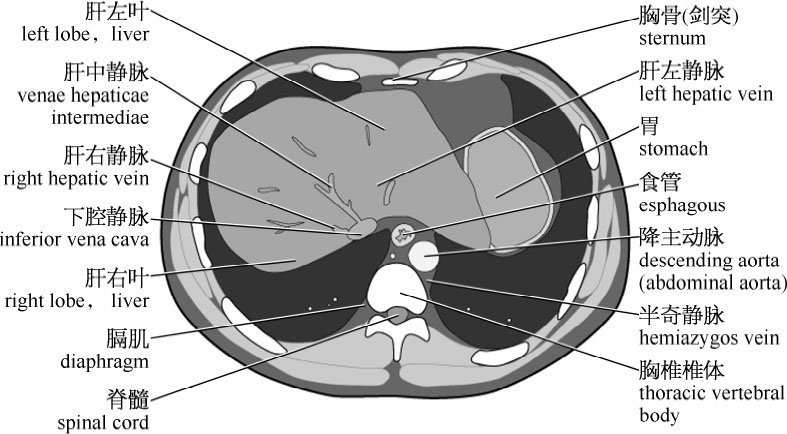
\includegraphics[width=0.7\textwidth]{./images/Image00010.jpg}
	\caption{心外膜脂肪组织增生及心肌脂肪浸润}
	\label{fig1-9}
\end{figure}
%\FloatBarrier 

(3)肾脂肪变性:贫血、缺氧、中毒和一些肾脏疾病时,肾曲管上皮细胞可发生脂肪变性。这是因为在上述疾病时肾小球毛细血管通透性增加,肾曲管特别是近曲小管上皮吸收漏出的脂蛋白,在细胞内分解成脂滴。脂滴空泡多位于近曲小管上皮细胞基底部或核周围。

脂肪变性发生的机制尚未完全清楚。一般认为与感染、中毒、缺氧等因素干扰或破坏细胞的脂肪代谢有关。具体作用途径则因病因不同而异。肝脂变的机制大致如下:①脂蛋白合成障碍,使脂肪堆积在肝细胞内不能转运出去。其原因常是缺乏合成脂蛋白的原料,如磷脂或组成磷脂的胆碱,或由于化学物或其他毒素破坏了内质网(蛋白合成部位)或抑制了某些酶的活性,使脂蛋白合成障碍。②脂肪酸氧化障碍。由于缺氧、感染、中毒,使线粒体受损,干扰β-氧化,使肝细胞含脂肪量增加。③进入肝细胞脂肪酸过多。例如饥饿或某些疾病造成饥饿状态,或糖尿病患者对糖的利用障碍,机体动用大量体脂,其中大部分以脂肪酸的形式进入肝脏,超过肝细胞将其氧化和合成脂蛋白的能力,于是在肝细胞内储积。

\paragraph{玻璃样变性}
玻璃样变性(hyaline
degeneration)又称透明变性,是指在HE染色情况下,细胞外间质或细胞质内出现伊红染、均质半透明、无结构的玻璃样物质。玻璃样变性其实为一组物理性状相同,但其发生原因、化学成分及机制各不相同的病理变化的统称。常见的玻璃样变性有三类:

(1)细胞内玻璃样变性:指细胞浆内出现大小不等、圆形、均质的红染小滴。细胞内玻璃样变性可由多种原因引起,如肾小球肾炎或其他疾病伴有明显蛋白尿时,肾近曲小管上皮细胞胞浆内可出现大小不等的圆形红染小滴,这是血浆蛋白经肾小球滤出而又被肾小管上皮细胞吞饮、融合而成的玻璃样小滴(图\ref{fig1-10}a)。慢性乙醇中毒时,由于细胞中间丝前角蛋白变性,肝细胞核周围的胞浆内可出现圆形或形状不甚规则的均质红染玻璃样物质,称为Mallory小体。

(2)结缔组织玻璃样变性:常发生在增生的纤维结缔组织,为胶原纤维老化的表现。肉眼观病变处呈灰白色,半透明,质地致密而坚韧(图\ref{fig1-10}b)。光镜下胶原蛋白交联、变性、融合,胶原纤维增粗并互相融合成索带状或片状的半透明均质物,纤维细胞明显减少。见于瘢痕组织、纤维化的肾小球、动脉粥样硬化的纤维斑块等。

(3)血管壁玻璃样变性:常发生于高血压病时的肾、脑、脾及视网膜的细动脉。这是由于细动脉持续痉挛,使内膜通透性增大,血浆蛋白渗入内膜,在内皮细胞下凝固成均匀红染玻璃样物质。如病变继续发展,血管壁平滑肌组织均被玻璃样物质替代而消失,再加上基底膜样物质增多,使病变血管壁增厚、变硬,管腔狭窄甚至闭塞,此即细动脉硬化症(图\ref{fig1-10}c),可引起肾、脑等器官缺血。
\begin{figure}[!htbp]
	\centering
	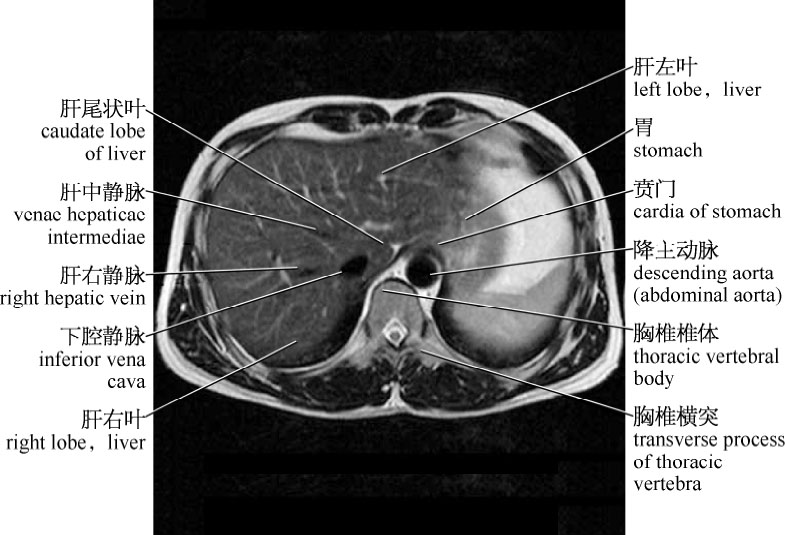
\includegraphics[width=0.7\textwidth]{./images/Image00011.jpg}
	\caption{不同类型玻璃样变性}
	\label{fig1-10}
\end{figure}
%\FloatBarrier

上述3种类型中,细胞内玻璃样变在病因去除后多能恢复,而后两者较难恢复。

\paragraph{黏液样变性}
组织间质内出现类黏液(黏多糖和蛋白质)的积聚称为黏液样变性(mucoid
degeneration)。镜下观:病变处细胞间质疏松,充以淡蓝色的胶状液体,其间散布一些多角形,星芒状的细胞,并以突起互相连缀。黏液样变性常见于间叶性肿瘤、急性风湿病时的心血管壁、动脉粥样硬化的血管壁。在甲状腺功能低下时,透明质酸酶活性受抑,含有透明质酸的黏液样物质及水分在皮下蓄积,形成黏液水肿。

\paragraph{淀粉样变}
组织内有淀粉样物质沉着称为淀粉样变(amyloid
degeneration)。淀粉样物质是蛋白质,其遇碘时可被染成棕褐色,再加硫酸后则变为蓝色,与淀粉染色特性相似,故称之为淀粉样变。此种病变可见于慢性炎症、内分泌系统肿瘤、老年性痴呆(Alzheimer病)等多种疾病。淀粉样物质的沉积可为局部性,亦可为全身性,常分布于细胞间或沉积在小血管基底膜下,还可沿组织纤维支架分布。镜下观:淀粉样物质呈淡伊红染色、均匀一致、云雾状。刚果红染色为橘红色(图\ref{fig1-11})。尽管形态相似,但在不同疾病时,淀粉样物质的化学本质不同,有的为免疫球蛋白,有的为激素,还有的为β{2}
淀粉样蛋白,等等。

\begin{figure}[!htbp]
	\centering
	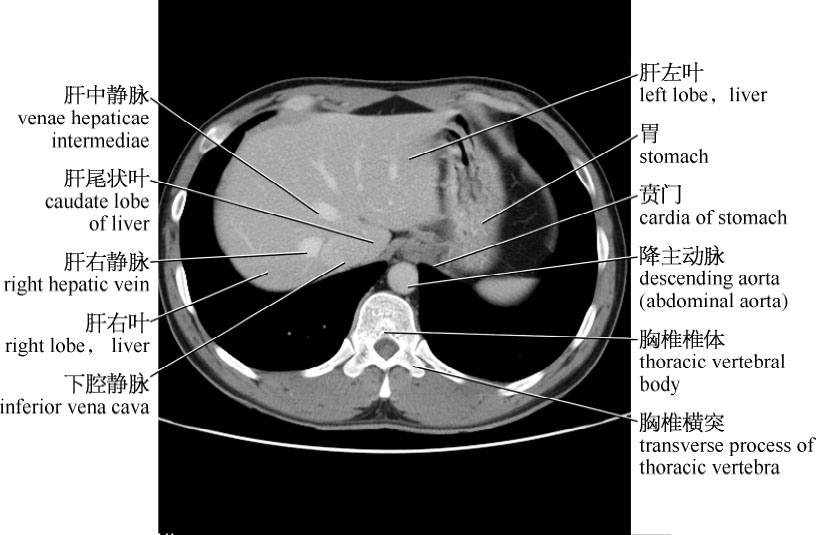
\includegraphics[width=0.7\textwidth]{./images/Image00012.jpg}
	\caption{肾小球淀粉样变}
	\label{fig1-11}
\end{figure}
%\FloatBarrier

\paragraph{病理性色素沉积}
细胞或组织内可有各种来自体内、体外的色素沉积,在病理情况下某些色素在体内会过量沉积。常见的病理性色素沉积有含铁血黄素、胆红素、脂褐素、黑色素。

(1)含铁血黄素(hemosiderin):系由铁蛋白微粒积聚而成的色素,颗粒状,棕黄或金黄色,具有折光性。此色素为血红蛋白被吞噬细胞溶酶体分解而成,如巨噬细胞破裂,则色素逸出于间质中。正常的骨髓组织或脾内可有少量含铁血黄素出现,在全身溶血性疾病时,含铁血黄素可沉积在全身的单核巨噬细胞系统内,组织出血时含铁血黄素常出现在出血灶附近。当左心衰竭导致肺淤血时,红细胞自肺泡壁毛细血管漏出于肺泡中,被巨噬细胞吞噬,肺泡腔内可出现吞噬含铁血黄素的巨噬细胞,又称为心力衰竭细胞。

(2)胆红素(bilirubin):也是在巨噬细胞内形成的一种血红蛋白衍生物,棕黄色或黄绿色。生理情况下,胆红素是衰老的红细胞被单核吞噬细胞分解后所形成。血中胆红素过多时,可将组织和体液染成黄色,称黄疸。因有血脑屏障,胆红素通常不能进入脑和脊髓,但在新生儿由于血脑屏障尚不完善,溶血性黄疸时,大量胆红素可进入脑细胞内,使其氧化磷酸化过程受损,能量产生受抑制,导致细胞变性,出现相应的神经症状。肉眼见豆状核、下丘脑、海马回等多处神经核明显黄染,故称之为核黄疸。胆红素一般呈溶解状态,但在胆道阻塞及某些肝脏疾病时也可为黄褐色折光性颗粒或团块,出现于肝细胞、Kupffer细胞、毛细胆管、小胆管等组织细胞内。

(3)脂褐素(lipofuscin):为一种黄褐色细颗粒状色素。其组成成分的50%为脂质,其余为蛋白质及其他物质。脂褐素系细胞内自噬溶酶体中的细胞器碎片发生了某种理化改变,不能被溶酶体酶消化而形成的一种不溶性残存小体。老年人及一些慢性消耗性疾病患者的肝细胞、肾上腺皮质网状带细胞和心肌细胞核两端的胞浆中可见到脂褐素,故又有消耗性色素之称。

(4)黑色素(melanin):为棕褐色或黑褐色的颗粒状色素,大小形状不一。正常人黑色素多存在于皮肤、毛发、虹膜及脉络膜的黑色素细胞内。它是由酪氨酸在黑色素细胞内的酪氨酸酶的作用下氧化、聚合而形成的一种不溶性聚合体。人脑垂体所分泌的ACTH能刺激黑色素细胞,促进黑色素形成。在肾上腺皮质功能低下时,对垂体的反馈抑制作用减弱,致使ACTH分泌增多,患者全身皮肤黑色素增多。局部黑色素增多常见于黑色素痣或恶性黑色素瘤等。

\paragraph{病理性钙化}
在病理情况下,骨和牙以外的组织内有固体钙盐的沉积,称为病理性钙化(pathologic
calcification)。主要成分为磷酸钙、碳酸钙及少量铁镁等物质。肉眼观:少量钙盐沉积难以辨认,仅在刀切组织时有砂粒感;量多时表现为白色石灰样颗粒或团块,质地坚硬。镜下观:HE染色切片中,钙盐呈蓝色颗粒状。病理性钙化可分为两种类型:

(1)营养不良性钙化:指钙盐沉积于变性、坏死的组织中或异物内,如结核坏死灶、脂肪坏死灶、动脉粥样硬化斑块的变性坏死区(图\ref{fig1-12}a),血栓、寄生虫体和虫卵。患者无全身钙、磷代谢障碍,血钙不高。这是一种较常见的病理性钙化,可能与局部碱性磷酸酶(来自坏死细胞及其周围组织内)升高有关。

\begin{figure}[!htbp]
	\centering
	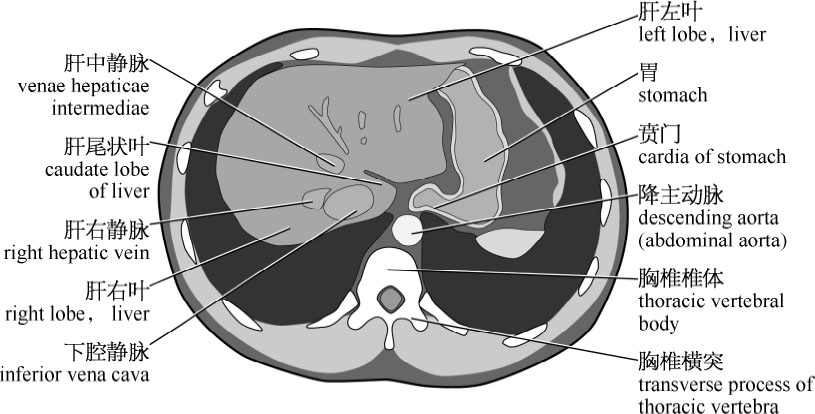
\includegraphics[width=0.7\textwidth]{./images/Image00013.jpg}
	\caption{动脉壁钙化}
	\label{fig1-12}
\end{figure}
%\FloatBarrier

(2)转移性钙化:较少见,是指由于全身钙、磷代谢障碍,血钙和(或)血磷升高,钙盐沉积于未受损的组织中。如甲状腺功能亢进或骨肿瘤造成骨组织破坏时,大量骨钙进入血液,使血钙升高,并沉积于肾小管、肺泡、胃黏膜和动脉壁中层(图\ref{fig1-12}b)。接受超剂量维生素D时,由于肠道对钙磷吸收明显增加,也可引起钙化。

钙化对机体的影响视具体情况而异。坏死组织钙化常是病灶愈合的表现,而血管壁的钙化则使管壁失去弹性、变硬、变脆,容易破裂出血。转移性钙化的危害性主要决定于原发病。

\subsubsection{不可逆性损伤-细胞死亡}

当细胞发生不可逆性代谢、结构和功能障碍,则引起细胞死亡(cell
death)。细胞死亡是病理学核心问题,其表现有两种方式:坏死与凋亡。坏死是细胞受到严重损伤时的病理性死亡过程,而凋亡多属生理性情况下发生的死亡,由细胞基因编程调控,在某些病理情况下,细胞死亡也可以凋亡形式出现。

\paragraph{坏死}
坏死(necrosis)是细胞受到严重损伤,以酶溶性变化为特点的活体内局部组织细胞的死亡。坏死可迅速发生,但在多数情况下由可逆性损伤逐渐发展而来。基本表现为细胞肿胀、细胞器崩解和蛋白质变性。

(1)坏死的基本病变

1)细胞核的改变:这是细胞坏死在形态学上的主要标志,表现为:①核浓缩(pyknosis),由于核脱水使染色质浓缩,嗜碱性染色增强,核体积缩小。②核碎裂(karyorrhexis),核染色质崩解为小碎片,核膜破裂,染色质碎片分散在胞质中。③核溶解(karyolysis),在DNA酶的作用下,染色质DNA分解,核乃失去对碱性染料的亲和力,因而染色变淡,仅见核轮廓,最后核消失(图\ref{fig1-13})。

\begin{figure}[!htbp]
	\centering
	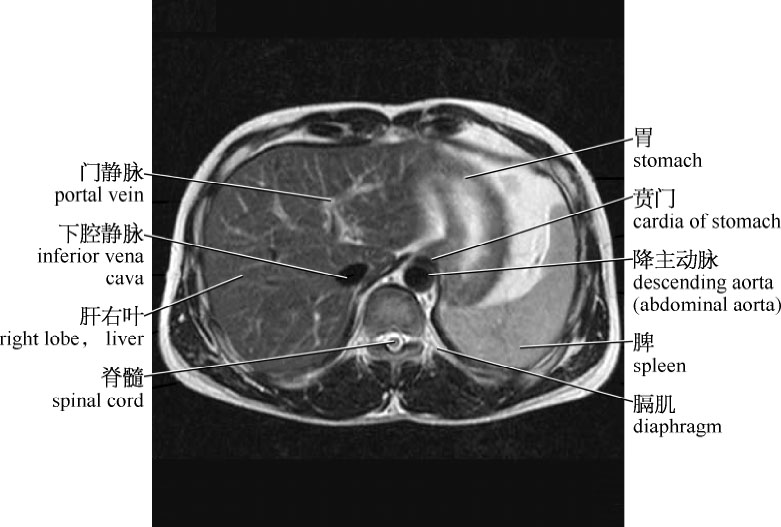
\includegraphics[width=0.7\textwidth]{./images/Image00014.jpg}
	\caption{细胞坏死时核的变化}
	\label{fig1-13}
\end{figure}

2)细胞浆的改变:由于细胞浆内嗜碱性核蛋白体减少或丧失,胞质变性蛋白质增多、糖原颗粒减少,使胞质对碱性染料苏木素的亲和力减少,而与酸性染料伊红的亲和力增强,致胞浆红染,坏死后期细胞浆崩解。

3)间质的改变:在实质细胞坏死后一段时间内,间质常无改变,以后在溶解酶的作用下,基质崩解,胶原纤维肿胀、断裂,继而崩解、液化。最后坏死的实质细胞和间质融合成一片无结构的颗粒状、红染物质,其内有时可见少量淡染的细胞核碎片。

由于坏死时细胞膜通透性增加,细胞内乳酸脱氢酶、琥珀酸脱氢酶、肌酸激酶、门冬氨酸氨基转移酶、丙氨酸氨基转移酶等被释放入血,造成细胞内酶活性降低而血浆中相应的酶活性升高,分别可作为诊断某些细胞(如肝、心肌、胰)坏死的参考指标。细胞内和血浆中酶活性的变化在坏死初即可检出,有助于细胞损伤早期诊断。

(2)坏死的病理类型:组织坏死后,由于酶的分解和蛋白质变性等因素综合作用的结果,使坏死组织出现不同的形态学变化,总体上可分为凝固性坏死、液化性坏死和特殊类型坏死等三个基本类型。

1)凝固性坏死(coagulation
necrosis):组织坏死后,蛋白质变性凝固且溶酶体酶水解作用较弱时,坏死区呈灰黄、干燥、质实状态,称为凝固性坏死。这种坏死多由缺血引起,常在心、肾、脾等器官的缺血性坏死时出现。
坏死灶周围常有暗红色出血带,与健康组织分界(图\ref{fig1-14}a)。
镜下特点:早期坏死灶细胞微细结构消失,但细胞组织的结构轮廓仍可保留一段时间(图\ref{fig1-14}b)。
最终坏死细胞崩解成碎片,被吞噬细胞吞噬或被游走进入的白细胞释放的溶解酶溶解。
凝固性坏死的发生机制仍不很清楚,可能是组织坏死后蛋白变性过程占优势,而水解酶的作用较少。

\begin{figure}[!htbp]
	\centering
	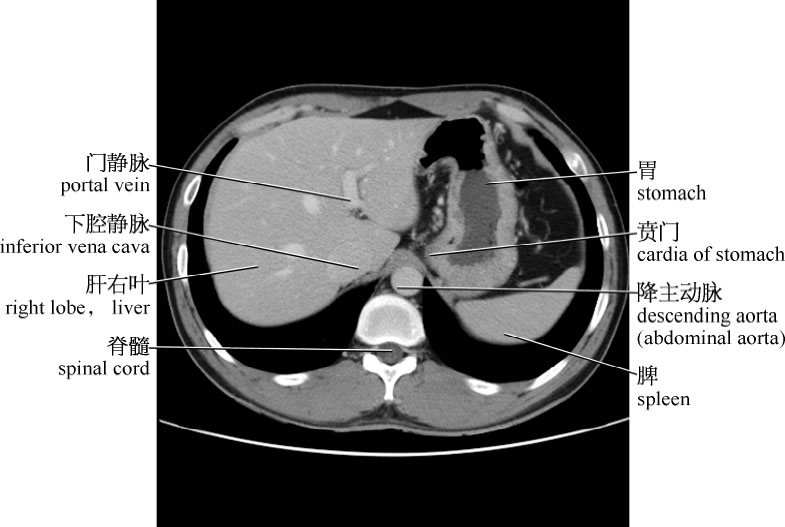
\includegraphics[width=.7\textwidth]{./images/Image00015.jpg}
	\caption{凝固性坏死}
	\label{fig1-14}
\end{figure}

2)液化性坏死(liquefaction
necrosis):组织坏死后分解、液化而呈液体状,有时还形成含有液体的腔。
如脑组织,坏死后分解成半流体状物质,又称为脑软化。
这种变化与脑组织水分和磷脂含量多,蛋白质含量少有关,故组织坏死后不易凝固而液化。
在某些病原体如化脓性细菌或溶组织阿米巴原虫能释放或产生蛋白溶解酶,可使组织发生液化性坏死。

3)特殊类型坏死

①干酪样坏死(caseous
necrosis):结核病时,坏死区内脂质较多,颜色带黄,质地松软,状似干酪,故称为干酪样坏死。
镜下观:坏死组织分解比较彻底,原有组织轮廓消失,呈现为一片红染、无定形的颗粒状物质(图\ref{fig1-15})。
梅毒性的坏死组织具有相似的形态,但其中的弹力纤维及血管结构仍可保留,致使坏死组织质地坚韧如树胶,故名树胶肿。
干酪样坏死不易吸收,一旦形成将存留较长时间。

\begin{figure}[!htbp]
	\centering
	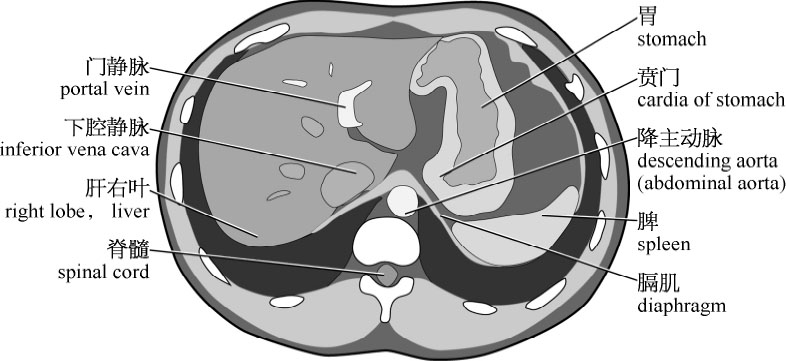
\includegraphics{./images/Image00016.jpg}
	\caption{肾干酪样坏死 \\ {\small 肾剖面可见多个黄白色干酪样坏死灶。}}
	\label{fig1-15}
\end{figure}

②纤维素样坏死(fibrinoid necrosis):旧称纤维素样变性(fibrinoid
degeneration)为发生于结缔组织胶原纤维和小血管壁的一种坏死。病变部位组织结构逐渐消失,变为一片境界不清的颗粒状、小条状或小块状无结构物质,经伊红染成深红色,由于其与纤维素染色性质相似,故名。常见于风湿病、结节性多动脉炎、新月体性肾小球肾炎、系统性红斑性狼疮等变态反应性疾病(图\ref{fig1-16})。也可见于恶性高血压病时的细动脉和胃溃疡底部动脉壁。其发生机制与抗原-抗体复合物引发的胶原纤维肿胀崩解、结缔组织免疫球蛋白沉积或血液纤维蛋白渗出变性有关。

\begin{figure}[!htbp]
	\centering
	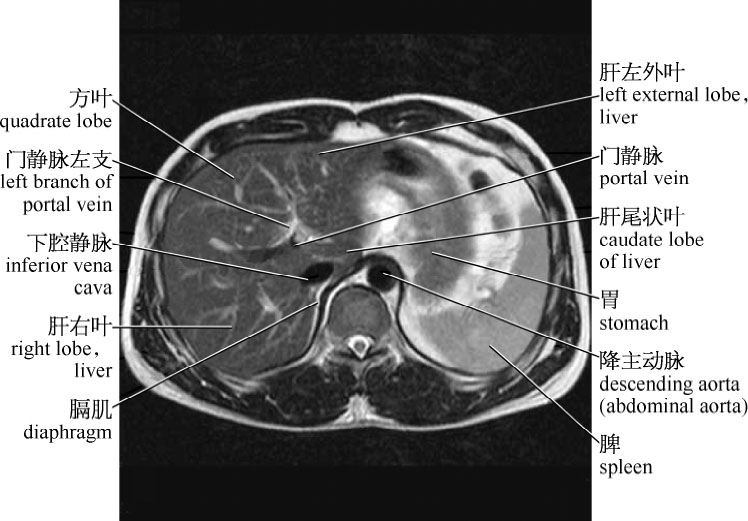
\includegraphics{./images/Image00017.jpg}
	\caption{肾小动脉壁纤维素样坏死(HE染色,高倍) \\ {\small 箭头所示深伊红染区为小动脉壁纤维素样坏死。}}
	\label{fig1-16}
\end{figure}


③脂肪坏死(fatty
necrosis):为液化性坏死的一种特殊类型,又可分为酶解性脂肪坏死和外伤性脂肪坏死。
前者常见于急性胰腺炎,由于胰脂酶外逸并被激活,对胰腺自身及腹腔的脂肪组织发生分解作用,形成的脂肪酸与组织内钙盐结合,在大网膜、后腹壁及肠系膜表面形成灰白色、质硬的不透明斑点或斑块,称为皂钙。
外伤性脂肪坏死常发生于富于脂肪组织的部位,乳腺尤其多见,有外伤史,局部表现为增大的肿块。镜下为大量的泡沫细胞及异物巨细胞。

④坏疽(gangrene):大块组织坏死后继发腐败菌感染,出现不同程度的腐败性变化。
腐败菌在分解坏死组织的过程中产生大量的硫化氢,并与血红蛋白分解释出的铁离子结合,形成硫化亚铁,致使坏死组织臭而发黑。
根据坏疽发生的部位、原因及形态特征不同,可分为干性、湿性、气性等类型。
干性坏疽(dry
gangrene)多发生于动脉阻塞而静脉回流仍然通畅的四肢末梢,坏死局部干燥、皱缩,呈黑色,与周围组织分界清楚(图\ref{fig1-17}),腐败性变化较轻。
湿性坏疽(moist
gangrene)常发生于与体外相连的内脏,如肠、阑尾等器官,也可发生于四肢。
形成的原因除动脉阻塞外,同时伴有局部淤血,坏死组织含水量多,适合腐败菌生长。
坏死区局部明显肿胀,呈深黄、暗绿或污黑,与周围组织无明显分界线,可引起严重的全身中毒症状。气性坏疽(gas
gangrene)也属于湿性坏疽。系深达肌肉的开放性创伤合并产气荚膜杆菌、腐败弧菌等厌氧菌感染。
细菌在分解液化组织的过程中产生大量气体,使坏死组织呈蜂窝状,压之有捻发感。
病变发展迅猛,沿肌束迅速蔓延。由于大量毒素被吸收,患者中毒症状十分严重,常需要紧急处理。

\begin{figure}[!htbp]
	\centering
	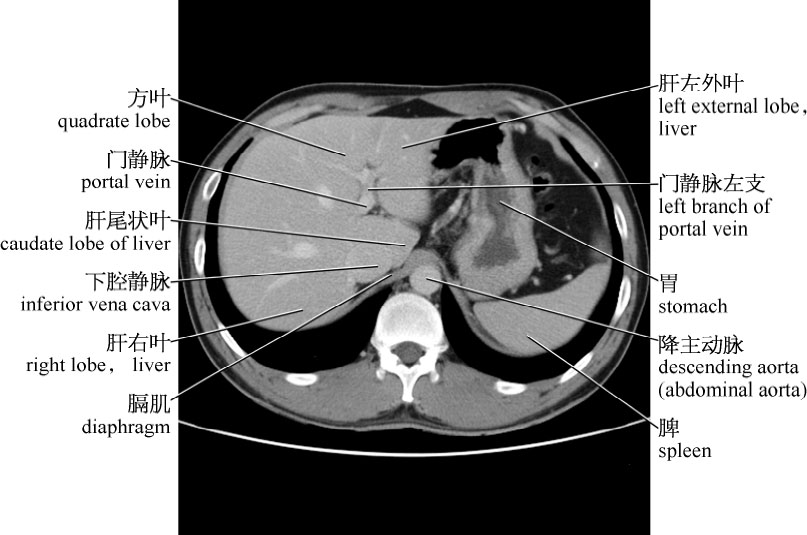
\includegraphics{./images/Image00018.jpg}
	\caption{足(干性)坏疽}
	\label{fig1-17}
\end{figure}

(3)坏死的结局:组织坏死后成了机体的异物,刺激周围组织,引起局部反应。不同的坏死组织结局不尽相同。

1)溶解吸收:坏死细胞自身或周围的炎细胞释放的溶解酶将坏死组织分解、液化,然后由淋巴管或小血管吸收,未被完全分解的组织碎片由吞噬细胞吞噬清除。坏死范围较大可形成囊腔。留下的组织缺损通过再生修复,这是机体处理坏死组织的基本方式。

2)分离排出:较大的坏死灶不易完全吸收,由于其周围发生炎症反应,其中的白细胞释放的溶解酶加速周边坏死组织溶解、吸收,使坏死灶与健康组织分离。位于皮肤、黏膜的坏死组织分离后脱落,留下局部缺损,浅者称为糜烂,深者称为溃疡。肾和肺脏的坏死组织分离后经自然管道排出,留下的空腔称为空洞。

3)机化与纤维包裹:坏死组织如不能被溶解吸收或分离排出,则由周围新生的毛细血管和成纤维细胞(合称肉芽组织)逐渐长入,取代坏死组织,最后形成瘢痕组织。这种由肉芽组织取代坏死组织(或其他异物、血凝块、血栓及渗出物等)的过程称为机化(organization)。如果坏死灶较大,难以吸收、机化,周边部增生的肉芽组织可将坏死灶包围,尔后肉芽组织转变为纤维组织,称为纤维包裹。机化和包裹的肉芽组织最终形成纤维瘢痕。

4)钙化:坏死组织和细胞碎片若未被及时清除,则日后易发生钙盐及其他矿物质沉积,引起营养不良性钙化。陈旧性干酪样坏死病灶或坏死的脂肪组织常有明显的钙化。

\paragraph{细胞凋亡}
细胞凋亡(apoptosis)也称程序性细胞死亡,是真核细胞在一定条件下通过启动其自身内部机制,主要是激活内源性核酸内切酶而发生的细胞主动性死亡方式。与细胞坏死不同,凋亡是一种主动过程,通常为单个细胞或小灶性细胞死亡,而不是大片实质细胞同时死亡。凋亡细胞周围无炎症反应,故有人借用希腊词“apoptosis”来形容其像秋天枯萎的树叶,从树干上悄无声息地飘零下来。

(1)形态特征:凋亡细胞有独特的形态特征。早期表现为细胞变圆,微绒毛及细胞突起消失,同时胞质浓缩,内质网扩张呈泡状,并与细胞膜融合形成细胞质小泡,向外隆起但无膜破裂;核染色质浓缩、凝聚于核膜下呈半月形。而后细胞膜内陷,自行分割为数个由胞膜包裹的、表面光滑的凋亡小体,其中含有大小不等的染色质片断、结构尚保持完整的细胞器和胞质成分(图\ref{fig1-18})。凋亡小体可与周围细胞分离,很快被邻近的细胞或巨噬细胞吞噬,在胞质溶酶体内迅速降解。

\begin{figure}[!htbp]
	\centering
	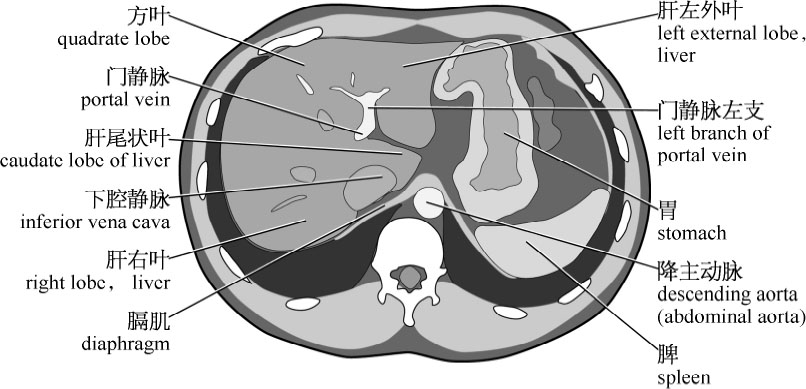
\includegraphics[width=.7\textwidth]{./images/Image00019.jpg}
	\caption{凋亡示意图}
	\label{fig1-18}
\end{figure}

(2)发生机制:细胞凋亡的发生机制十分复杂,它是一种由某些刺激因子启动、内在基因调控,并依赖能源的连锁分子事件,其中有信号传导、特异性调节分子作用、共同蛋白酶(caspases,半胱氨酸天冬氨酸蛋白酶,亦称胱冬肽酶)家族活化及死亡细胞的被噬和移去等过程,故曾有程序性死亡(programmed
cell death)之称。

刺激因子不同,其信号通路、调节分子种类不尽相同。目前已知,在人体各种病理过程中,发生细胞凋亡的主要通路有两条(图\ref{fig1-19}):一是线粒体通路或内源通路;二是死亡受体通路或外源通路。

\begin{figure}[!htbp]
	\centering
	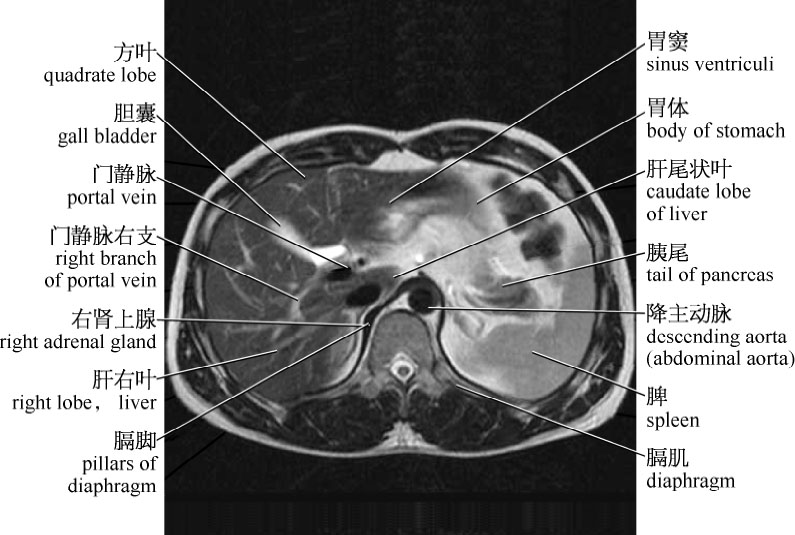
\includegraphics[width=.7\textwidth]{./images/Image00020.jpg}
	\caption{细胞凋亡机制示意图}
	\label{fig1-19}
\end{figure}

线粒体通透性决定细胞是否凋亡,而通透性受控于含20个以上蛋白成员的Bcl-2家族。当细胞失去生长因子或生存信号、暴露于DNA损伤因子(如紫外线、放射线、活性氧和细胞毒药物等)以及细胞内堆积过多的错误折叠蛋白时,Bcl-2家族感应分子即被活化,继之活化该家族另外两个成员(效应分子)-Bax和Bak,它们形成二聚体并插入线粒体膜,使后者通透性增加,细胞色素C和其他蛋白分子逸出线粒体进入胞浆,令激发性胱冬肽酶(caspase
9)活化,后者再使效应性胱冬肽酶(caspase
3、6、7)活化,最终导致细胞骨架蛋白崩解、核酸内切酶活化和凋亡小体形成。Bcl-2、Bcl-x{L}
抑制Bax和Bak活化,故可阻断凋亡。

细胞凋亡的死亡受体通路涉及肿瘤坏死因子(TNF)及其受体(TNFR)、FAS-FAS配体作用等。受体的胞内段为死亡功能区(dead
domain)。一旦受体配体结合,死亡信号即通过死亡功能区和相关的适配蛋白(adapter
protein)传递至激发性胱冬肽酶(caspase
8),并使之活化。后续反应与线粒体通路相同。

(3)细胞凋亡与坏死的区别:细胞凋亡的发生机制与前述的坏死不同,有相关基因调节。其中Fas、Bax、P53等基因有促进作用,Bcl-2、Bcl-x{L}
等有抑制凋亡作用。凋亡细胞内源性Ca{2+} 、Mg{2+}
依赖DNA内切酶的激活,从而切割核小体间DNA,形成不连续的180~200
bp或其倍数的DNA片断。被切割的DNA片断在琼脂糖凝胶电泳时表现为阶梯状电泳条带,这种现象被认为是细胞凋亡的可靠指标。凋亡的细胞质膜完整,无细胞内容物溢出,不引起细胞周围炎症反应,也不诱发周围细胞的增生修复。细胞凋亡和细胞坏死的区别见表\ref{tab1-1}。

\begin{table}[ht]
	\caption{细胞凋亡和细胞坏死的区别}
	\label{tab1-1}
	\centering
	\begin{tabular}{lp{5cm}p{5cm}}
		\toprule
		         & 细胞凋亡                                                                           & 细胞坏死                       \\
		\midrule
		形态特征 & 细胞固缩,核染色质边集、细胞膜及各细胞器膜完整,膜可发泡出芽,形成调亡小体
		         & 细胞显著肿胀,核染色质絮状或边集,细胞膜及各细胞器膜溶解破裂,溶酶体释放,细胞溶解                                  \\
		生化特征 & 核酸内切酶活化,半胱氨酸蛋白酶活化,谷氨酰谷氨酰转移酶活性增高
		         & 核酸内切酶无活化,半胱氨酸蛋白酶、转移酶活性无变化                                                                  \\
		DNA电泳  & 阶梯状条带                                                                         & 弥散分布的电泳拖带             \\
		炎症反应 & 无                                                                                 & 有                             \\
		机制     & 由凋亡相关基因调控主动进行(自杀性)                                                 & 与基因调控无关被动进行(他杀性) \\
		发生条件 & 多为生理性                                                                         & 病理性                         \\
		\bottomrule
	\end{tabular}
\end{table}


(4)细胞凋亡的生理、病理意义:细胞凋亡是最基本的生物现象,是机体生存和发育的基础。大量研究材料显示它涉及生命活动中的许多领域,包括发育、生长、造血、免疫、肿瘤发生等。通过凋亡可以清除多余的、无用的细胞。胚胎发育过程中,一些遗迹如人胚的尾芽和鳃随发育定期消亡,就是通过凋亡的方式进行的。细胞凋亡也可作为机体的自身保护机制,以清除发育不正常及对机体有害的细胞,畸胎瘤就是未彻底凋亡的残留胚层结构存留所致。B和T细胞发育成熟过程中本该发生凋亡的细胞保留下来将形成自身抗原,导致自身免疫病;细胞凋亡的异常改变包括凋亡不足或凋亡过度都可引起一些疾病。T辅助细胞($\text{CD}^+_4$
)在人类免疫缺陷病毒(HIV)感染后,发生凋亡,从而导致获得性免疫缺陷病。细胞凋亡的调控失常与肿瘤的发生关系密切,当机体某个基因发生突变而导致凋亡信号下调凋亡不足时,可引起细胞异常增生而发生肿瘤。目前临床上已开始用药物或放射线来诱导肿瘤细胞凋亡以达到治疗肿瘤的目的。

\begin{center}
	\textbf{知识链接}
\end{center}
\chapterabstract{自噬(autophagy)是细胞对自身细胞器或胞内聚集的变性蛋白等大分子物质进行包裹以及降解消化的现象。近年发现自噬不足或过度均可导致细胞死亡,所以被称为第三种细胞死亡方式。}

生理状态下,细胞通过自噬来清除受损、衰老和失去功能的细胞器及各种大分子物质,最终降解产物再循环利用,为细胞重建和再生提供原料。病理状态下,自噬不仅能保护细胞免受毒物损伤,而且能抵御病原体的侵害。在机体的免疫、感染、炎症、肿瘤、心血管病和神经退行性疾病的发生发展过程中均发挥重要作用。自噬和凋亡有相似之处,如二者共享某些调节蛋白,如胱冬肽酶。某些刺激因素既可诱导自噬亦可引起凋亡。

总之,疾病源于组织细胞的损伤,内外因子的刺激强度不同,损伤程度不同(图\ref{fig1-20})。若刺激在细胞能承受范围内,则表现为适应,属轻度损伤,细胞可出现萎缩、增生、肥大和化生等形态学改变。若刺激时间长强度大,细胞将发生显著损伤,出现细胞内外异常物质沉积,甚至坏死;若刺激因素激活特殊信号系统,细胞可发生凋亡。

\begin{figure}[!htbp]
	\centering
	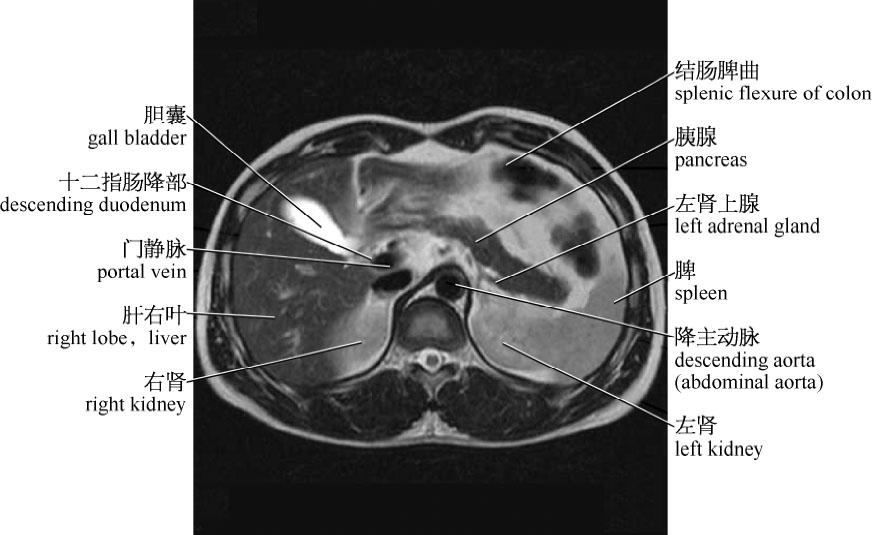
\includegraphics{./images/Image00023.jpg}
	\caption{组织细胞适应、损伤概览}
	\label{fig1-20}
\end{figure}

\section*{复习与思考}

{一、名词解释}

适应 萎缩 肠上皮化生 细胞水肿 脂肪变性 虎斑心 病理性钙化 凝固性坏死 干酪样坏死 液化性坏死 脑软化 坏疽 细胞凋亡

{二、问答题}

1. 机体组织细胞可出现哪几种适应性改变?

2. 久病卧床后肢体变细属于哪种类型的萎缩?为什么?

3. 试述肝脂变的原因和病变。

4. 何谓玻璃样变?好发于哪些部位?

5. 体内常见的色素有哪些?光镜下的特点是什么?

6. 试述坏死的镜下特点及结局。

7. 细胞的坏死和凋亡如何区别?


\chapter{免疫系统}
\begin{framed}
\noindent\textbf{【知识体系】}

\begin{center}
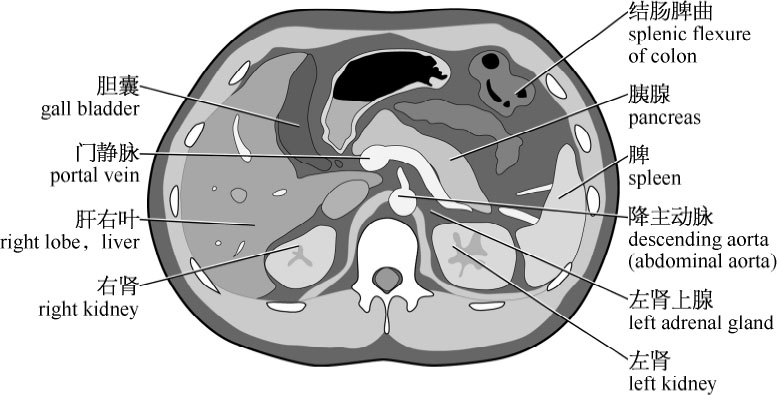
\includegraphics[width=.66\textwidth]{./images/Image00025.jpg}
\end{center}

\noindent\textbf{【课前思考】}

与机体的其他组织系统一样,免疫系统由哪些组织、器官、细胞组成?各种器官、细胞有何特征?在维护我们机体健康中各自起到怎样的作用?当有病原微生物入侵时,机体的各种免疫细胞是怎样各司其职又相互协调的?机体的免疫系统与国家的防御体系有何相似之处?

\noindent\textbf{【本章重点】}

1.免疫系统的构成;

2.免疫器官、免疫细胞的功能。

\noindent\textbf{【教学目标】}

1.掌握免疫系统组成:免疫器官(中枢免疫器官、外周免疫器官)、免疫细胞、免疫分子;

2.掌握中枢免疫器官的组成:骨髓、胸腺的主要免疫功能;

3.掌握外周免疫器官与组织的组成:淋巴结、脾脏的主要免疫功能。
\end{framed}
机体抵御外界病原微生物的入侵有三道防卫系统:

1.皮肤、黏膜及其分泌物

皮肤黏膜的机械阻挡作用和附属物(如纤毛)的清除作用,皮肤黏膜分泌物(如汗腺分泌的乳酸、胃黏膜分泌的胃酸等)的杀菌作用,体表和与外界相通的腔道中寄居的正常微生物丛对入侵微生物的拮抗作用等,属于机体第一道防线。其次是内部屏障。抗原物质一旦突破第一道防线进入机体后,即遭到机体内部屏障的清除,包括:淋巴和单核吞噬细胞系统屏障、正常体液中的一些非特异性杀菌物质、血脑屏障和胎盘屏障等(图\ref{fig2-1})。

\begin{figure}[!htbp]
 \centering
 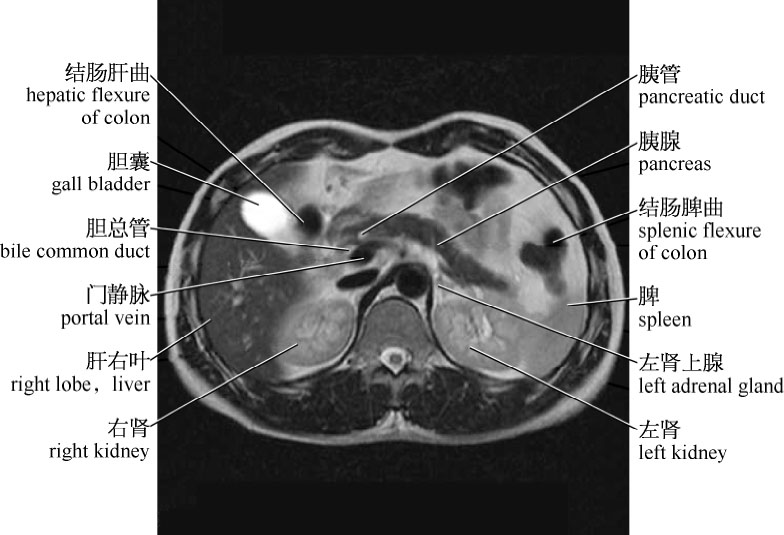
\includegraphics[width=.6\textwidth]{./images/Image00026.jpg}
 \caption{机体第一道防线}
 \label{fig2-1}
  \end{figure} 

2.吞噬细胞、NK细胞、抗菌蛋白、炎症应答------淋巴系统

微生物进入机体组织以后,多数沿组织细胞间隙的淋巴液经淋巴管到达淋巴结,但淋巴结内的巨噬细胞会消灭它们,阻止它们在机体内扩散,这就是淋巴屏障作用。如果微生物数量大、毒力强,就有可能冲破淋巴屏障,进入血液循环,扩散到组织器官中去。这时,它们会受到单核吞噬细胞系统屏障的阻挡。这是一类大的吞噬细胞。机体内还有一类较小的吞噬细胞,其中主要的是中性粒细胞和嗜酸性粒细胞。它们不属于单核吞噬细胞系统,但与单核吞噬细胞系统一样,分布于全身,对入侵的微生物和大分子物质有吞噬、消化和消除的作用。

在正常体液中的一些非特异性杀菌物质,如补体、调理素、溶菌酶、干扰素、乙型溶素、吞噬细胞杀菌素等,也与淋巴和单核吞噬细胞系统屏障一样,是机体的第二道防线,有助于消灭入侵的微生物(图\ref{fig2-2})。

\begin{figure}[!htbp]
 \centering
 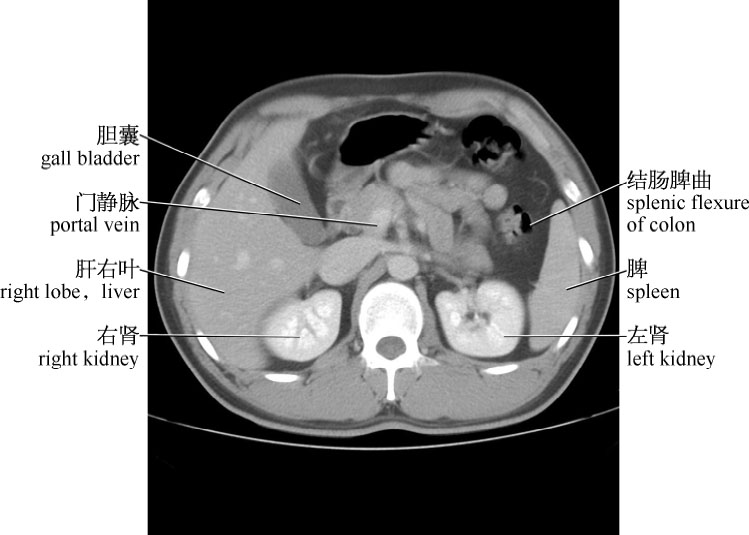
\includegraphics[width=.6\textwidth]{./images/Image00027.jpg}
 \caption{机体的第二道防线}
 \label{fig2-2}
  \end{figure} 

3.免疫系统:淋巴细胞、抗体;特点:特异性、多样性、记忆性、识别自我与非我(图\ref{fig2-3})。

\begin{figure}[!htbp]
 \centering
 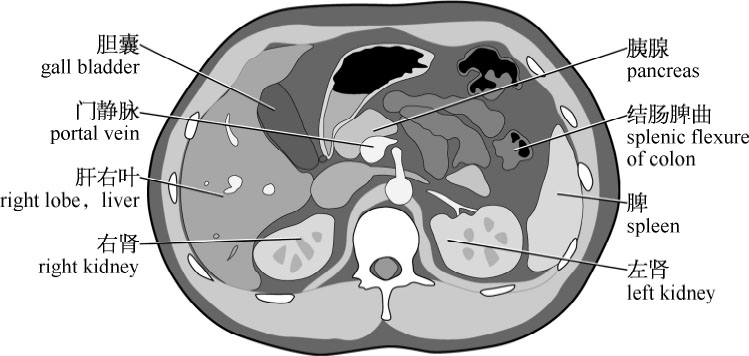
\includegraphics[width=.5\textwidth]{./images/Image00028.jpg}
 \caption{机体的第三道防线------免疫系统}
 \label{fig2-3}
  \end{figure} 

我们主要讲授免疫系统。

免疫系统(immune
system)乃承担免疫功能的组织系统,是机体对抗原刺激产生应答、执行免疫效应的物质基础。从宏观至微观进行描述,免疫系统包括免疫器官(中枢免疫器官和外周免疫器官)、免疫细胞(造血干细胞、淋巴细胞、单核吞噬细胞及其他免疫细胞)和免疫分子(抗体、补体、细胞因子)。

\section{中枢免疫器官}

中枢免疫器官(central immune
organ)是免疫细胞发生、分化、发育、成熟的场所,并对外周免疫器官的发育起主导作用,某些情况下(如再次抗原刺激或自身抗原刺激)也是产生免疫应答的场所。人和其他哺乳类动物的中枢免疫器官包括骨髓、胸腺,鸟类腔上囊(法氏囊)的功能相当于骨髓。


\subsection{骨髓}

骨髓(bone
marrow)是重要的中枢免疫器官,可分为红骨髓和白骨髓。红骨髓由结缔组织、血管、神经和实质细胞组成,呈海绵样存在于骨松质的腔隙中,具有活跃的造血功能。骨髓功能的发挥与其微环境有密切关系。骨髓微环境指造血细胞周围的微血管系统、末梢神经、网状细胞、基质细胞以及它们所表达的表面分子和所分泌的细胞因子。这些微环境组分是介导造血干细胞黏附、分化发育、参与淋巴细胞迁移和成熟的必需条件。骨髓是人和哺乳动物的造血器官(图\ref{fig2-4})。它具有如下功能:

1.各类免疫细胞发生的场所:骨髓造血干细胞具有分化成不同血细胞的能力,故被称为多能造血干细胞(multiple
hematopoietic stem
cell,HSC)。在骨髓微环境中,HSC首先分化为髓样前体细胞(myeloid
progenitor)和淋巴样前体细胞(lymphoid
progenitor)。髓样前体细胞最终分化成为粒细胞、单核细胞、红细胞、血小板;淋巴样前体细胞分化为T淋巴细胞(简称T细胞)、B淋巴细胞(简称B细胞)和自然杀伤细胞(NK细胞)。

\begin{figure}[!htbp]
 \centering
 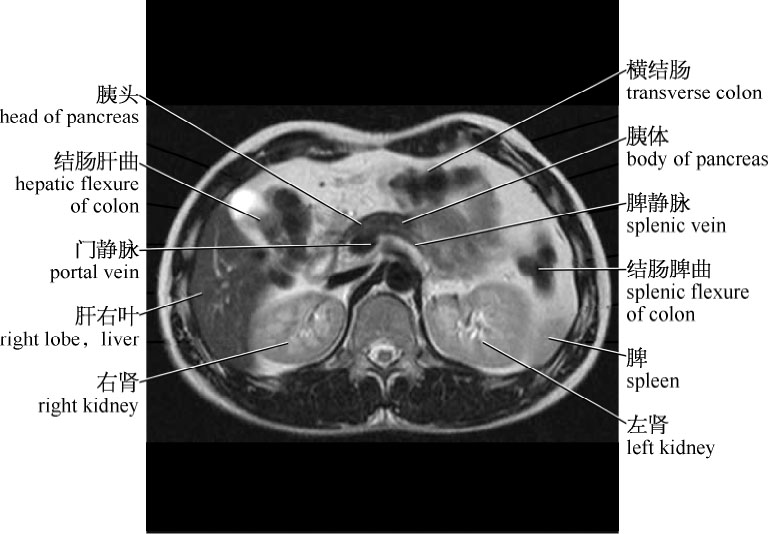
\includegraphics[width=.6\textwidth]{./images/Image00029.jpg}
 \caption{血细胞发育示意图}
 \label{fig2-4}
  \end{figure} 

2.B细胞分化成熟的场所:骨髓中产生的淋巴样前体细胞循不同的途径分化发育:一部分经血液迁入胸腺,发育成熟为成熟的T细胞;另一部分则在骨髓内继续分化为成熟B细胞。与T细胞在胸腺中分化的过程类似,B细胞在骨髓中也发生抗原受体(B
cell
receptor,BCR)等表面标志的表达、选择性发育或凋亡等。成熟的B细胞进入血循环,最终也定居在外周免疫器官。

3.发生B细胞应答的场所:骨髓是发生再次体液免疫应答的主要部位,外周免疫器官中的记忆性B细胞在抗原刺激下被活化,经淋巴液和血液进入骨髓后分化成熟为浆细胞,并产生大量抗体释放至血液循环。外周免疫器官中所发生的再次应答,其产生抗体的速度快,但持续时间短;而骨髓中所发生的再次应答,其产生抗体的速度慢,但可缓慢、持久地产生大量抗体,从而成为血清抗体的主要来源。

最新研究成果表明:在一定的微环境中,骨髓中的造血干细胞和基质干细胞还可分化为其他组织的多能干细胞(如神经干细胞、心肌干细胞等),这一突破性的进展开拓了骨髓生物学作用的全新领域,并可望在组织工程和临床医学中得到广泛应用。


\subsection{胸腺}

\begin{figure}[!htbp]
 \centering
 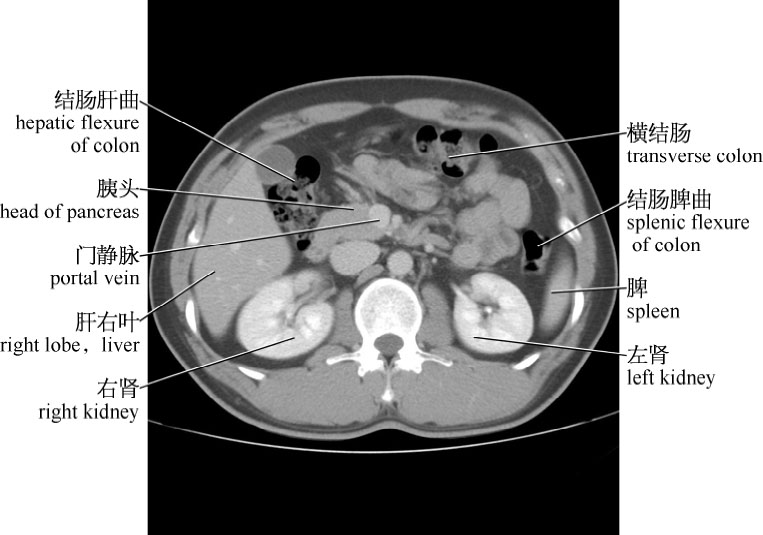
\includegraphics[width=0.5\textwidth]{./images/Image00030.jpg}
 \caption{人的胸腺}
 \label{fig2-5}
  \end{figure} 

人的胸腺(thymus)随年龄不同而有明显差别(图\ref{fig2-5})。新生期胸腺重量约15~20g;以后逐渐增大,青春期可达30~40g,其后随年龄增长而逐渐萎缩退化;老年期胸腺明显缩小,大部分被脂肪组织所取代。胸腺是T细胞分化、成熟的场所,其功能状态直接决定机体细胞免疫功能,并间接影响体液免疫功能。

(一)胸腺的解剖结构

胸腺的结构如图\ref{fig2-6}所示。一结缔组织被膜覆盖胸腺表面,并深入胸腺实质将其分隔成许多小叶。小叶的外层为皮质(cortex),内层为髓质(medulla),皮髓质交界处含大量血管,皮质内85\%~90\%的细胞为未成熟T细胞(即胸腺细胞),也存在少量上皮细胞、巨噬细胞(macrophage,Mφ)和树突状细胞(dendritic
cell,DC)等。胸腺浅皮质内发育早期的胸腺上皮细胞也称抚育细胞(nurse
cell),其在胸腺细胞分化中发挥重要作用。髓质内含大量上皮细胞和疏散分布的胸腺细胞、Mφ和DC。

\begin{figure}[!htbp]
 \centering
 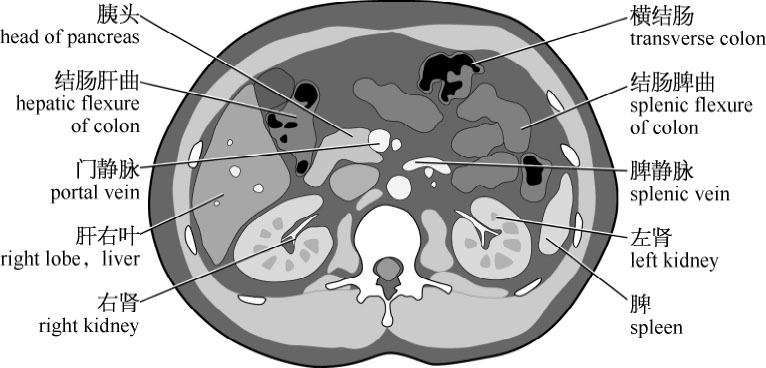
\includegraphics[width=0.7\textwidth]{./images/Image00031.jpg}
 \caption{胸腺结构示意图}
 \label{fig2-6}
  \end{figure} 

(二)胸腺的细胞组成:主要由胸腺基质细胞和胸腺细胞组成

1.胸腺基质细胞(thymic stromal cell,TSC):TSC以胸腺上皮细胞(thymus
epithelial
cell,TEC)为主,还包括巨噬细胞、DC及成纤维细胞等。TSC互相连接成网,并表达多种表面分子和分泌多种胸腺激素,从而构成重要的胸腺内环境。其中,抚育细胞与胸腺细胞通过各自表达的黏附分子密切接触,为胸腺细胞的发育提供必需的信号。

2.胸腺细胞:骨髓产生的前T细胞经血循环进入胸腺,即成为胸腺细胞。不同分化阶段的胸腺细胞其形态学、表面标志等各异,并可按其CD4、CD8表达情况分为4个亚群,即:CD4\textsuperscript{-}
CD8\textsuperscript{-} 、CD4\textsuperscript{+} CD8\textsuperscript{+}
、CD4\textsuperscript{+} CD8\textsuperscript{-} 、CD4\textsuperscript{-}
CD8\textsuperscript{+} 。

(三)胸腺微环境

胸腺微环境由TSC、细胞外基质及局部活性物质组成,其在胸腺细胞分化过程的不同环节均发挥重要作用。胸腺上皮细胞是胸腺微环境的最重要组分,其参与胸腺细胞分化的机制为:

1.分泌胸腺激素和细胞因子:主要的胸腺激素有胸腺素(thymosin)、胸腺刺激素(thymulin)、胸腺体液因子(thymic
humoral factor)、胸腺生成素(thymopoietin,TP)、血清胸腺因子(serum
thymic
factor)等。它们分别具有促进胸腺细胞增殖和分化、发育等功能。胸腺基质细胞还可产生多种细胞因子,它们通过与胸腺细胞表面相应受体结合,调节胸腺细胞发育和细胞间相互作用。上述胸腺激素和细胞因子是诱导胸腺细胞分化为成熟T细胞的必要条件。

2.与胸腺细胞相互接触:此乃通过上皮细胞与胸腺细胞间表面黏附分子及其配体、细胞因子及其受体、抗原肽-MHC分子复合物与TCR等相互作用而实现。

细胞外基质(extracellular
matrix)也是胸腺微环境的重要组成部分,它们可促进上皮细胞与胸腺细胞接触,并参与胸腺细胞在胸腺内移行成熟。

(四)胸腺的功能

1.T细胞分化、成熟的场所:胸腺是T细胞发育的主要场所。在胸腺产生的某些细胞因子作用下,来源于骨髓的前T细胞被吸引至胸腺内成为胸腺细胞。胸腺细胞循被膜下转移到皮质再向髓质移行,并经历十分复杂的选择性发育。在此过程中,约95\%的胸腺细胞发生以凋亡(apoptosis)为主的死亡而被淘汰,仅不足5\%的细胞分化为成熟T细胞。其特征为:表达成熟抗原受体(TCR)的CD4或CD8单阳性细胞;获得MHC限制性的抗原识别能力;获得自身耐受性。发育成熟的T细胞进入血循环,最终定居于外周免疫器官。

近期研究证实,胸腺并非T细胞分化发育的唯一场所。例如T细胞可在胸腺外组织(如肠道黏膜上皮、皮肤组织及泌尿生殖道黏膜组织等)中发育成熟。另外,肝脏也可能是某些T细胞分化发育的场所。

2.免疫调节功能:胸腺基质细胞可产生多种肽类激素,它们不仅促进胸腺细胞的分化成熟,也参与调节外周成熟T细胞。

3.屏障作用:皮质内毛细血管及其周围结构具有屏障作用,阻止血液中大分子物质进入,此为血-胸腺屏障(blood-thymus
barrier)。


\subsection{腔上囊}

腔上囊又称法氏囊(bursa of
fabricius),是鸟类动物特有的淋巴器官,位于胃肠道末端泄殖腔的后上方(图\ref{fig2-7})。与胸腺不同,腔上囊训化B细胞成熟,主导机体的体液免疫功能。将孵出的雏鸡去掉腔上囊,会使血中γ球蛋白缺乏,且没有浆细胞,注射疫苗亦不能产生抗体。人类和哺乳动物没有法氏囊,其功能由相似的组织器官代替,称为法氏囊同功器官;曾一度认为同功器官是阑尾、扁桃体和肠集结淋巴结,现在已证明是骨髓。

\begin{figure}[!htbp]
 \centering
 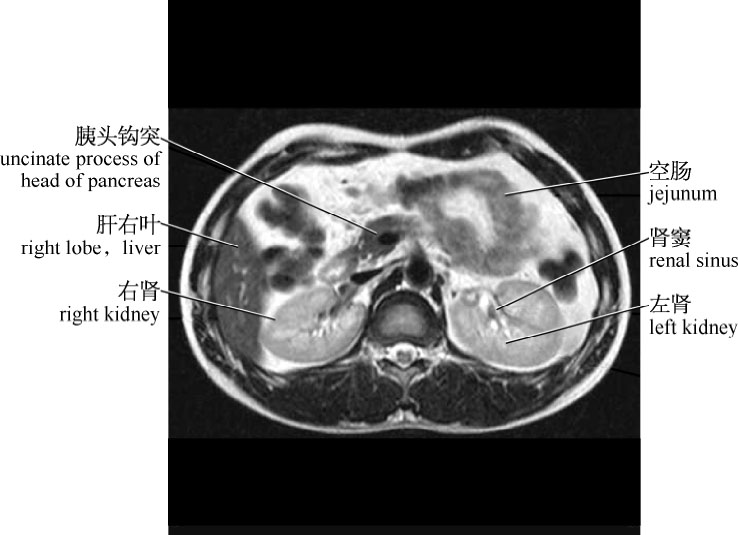
\includegraphics[width=.5\textwidth]{./images/Image00032.jpg}
 \caption{鸡的胸腺和法氏囊}
 \label{fig2-7}
  \end{figure} 

\section{外周免疫器官}

外周免疫器官(peripheral immune
organ)包括脾、淋巴结、淋巴样小结、扁桃体、阑尾等,这些器官内富含能捕捉和处理抗原的巨噬细胞和树突状细胞,以及能介导免疫反应的T细胞和B细胞。


\subsection{淋巴结}

淋巴结(lymph node)广泛分布于全身非黏膜部位的淋巴通道上。

(一)淋巴结的结构

淋巴结的结构如图\ref{fig2-8}所示,淋巴结表面覆盖有结缔组织被膜,后者深入实质形成小梁。淋巴结分为皮质和髓质两部分,彼此通过淋巴窦相通。被膜下为皮质,包括浅皮质区、副皮质区和皮质淋巴窦。

浅皮质区又称为非胸腺依赖区(thymus-independent
area),是B细胞定居的场所,该区内有淋巴滤泡(或称淋巴小结)。未受抗原刺激的淋巴小结无生发中心,称为初级滤泡(primary
follicle),主要含静止的成熟B细胞;受抗原刺激的淋巴小结内出现生发中心(germinal
center),称为次级滤泡(secondary
follicle),内含大量增殖分化的B淋巴母细胞,此细胞向内转移至淋巴结中心部髓质,即转化为可产生抗体的浆细胞。

副皮质区又称胸腺依赖区(thymus-dependent
area),位于浅皮质区和髓质之间,为深皮质区,是T细胞(主要是CD\textsuperscript{+}
\textsubscript{4}
T细胞)定居的场所。该区有许多由内皮细胞组成的毛细血管后微静脉,也称高内皮细胞小静脉(high
endothelial venule,HEV),在淋巴细胞再循环中起重要作用。

髓质由髓索和髓窦组成。髓索内含有
B细胞、T细胞、浆细胞、肥大细胞及Mφ。髓窦内Mφ较多,有较强滤过作用。

\begin{figure}[!htbp]
 \centering
 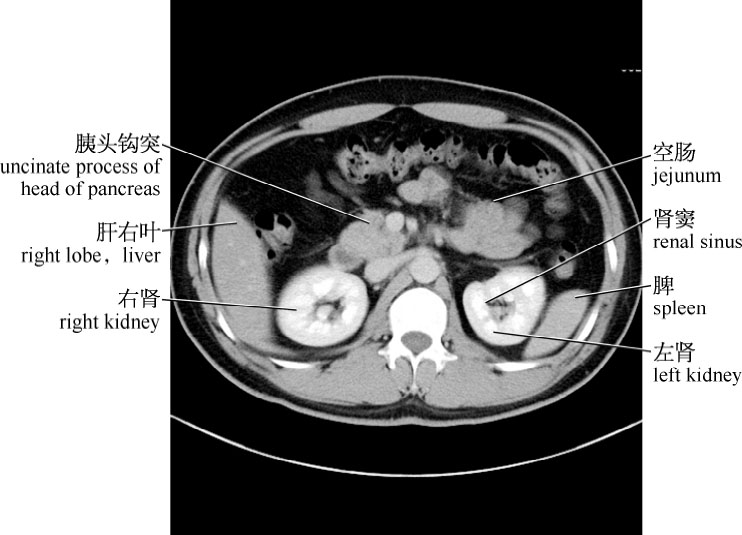
\includegraphics[width=.6\textwidth]{./images/Image00033.jpg}
 \caption{淋巴结的结构}
 \label{fig2-8}
  \end{figure} 

(二)淋巴结的功能

1.T 细胞及
B细胞定居的场所:分别在胸腺和骨髓中分化成熟的T、B细胞,均可定居于淋巴结。其中,T细胞占淋巴结内淋巴细胞总数的75\%,B细胞占25\%。

2.免疫应答发生的场所:抗原递呈细胞携带所摄取的抗原进入淋巴结,将已被加工、处理的抗原递呈给淋巴结内的T细胞和B细胞,使之活化、增殖、分化,故淋巴结是发生细胞免疫和体液免疫应答的主要场所。

3.参与淋巴细胞再循环:淋巴结深皮质区的HEV在淋巴细胞再循环中发挥重要作用,血循环中的淋巴细胞穿越HEV壁进入淋巴结实质,然后通过输出淋巴管进入胸导管或右淋巴管,再回到血液循环。

4.过滤作用:组织中的病原微生物及毒素等进入淋巴液,其缓慢流经淋巴结时,可被Mφ吞噬或通过其他机制被清除。因此,淋巴结具有重要的滤过作用。


\subsection{脾脏}

(一)脾脏的结构

脾脏的结构如图\ref{fig2-9}所示,脾脏(spleen)是人体最大的淋巴器官,可分为白髓、红髓和边缘区三部分。白髓由密集的淋巴组织构成,包括动脉周围淋巴鞘和淋巴小结。动脉周围淋巴鞘为T细胞居住区;鞘内的淋巴小结为B细胞居住区,未受抗原刺激为初级滤泡,受抗原刺激后出现生发中心,为次级滤泡。红髓分布于白髓周围,包括髓索和髓窦:前者主要为B细胞居留区,也含Mφ和DC;髓窦内为循环的血液。白髓与红髓交界处为边缘区(marginal
zone),是血液及淋巴细胞进出的重要通道。

\begin{figure}[!htbp]
 \centering
 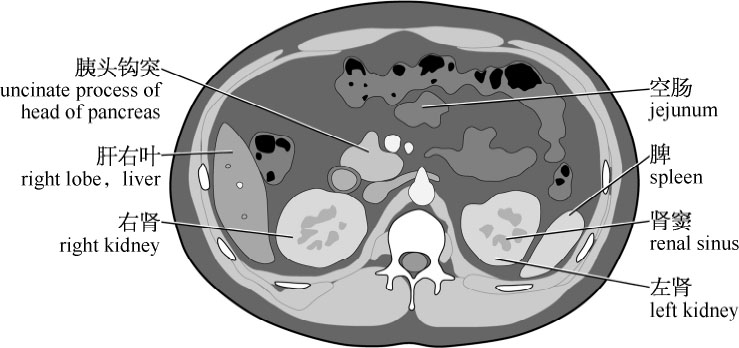
\includegraphics[width=.5\textwidth]{./images/Image00034.jpg}
 \caption{脾脏的结构}
 \label{fig2-9}
  \end{figure} 

(二)脾脏的功能

脾脏是重要的外周免疫器官,脾切除的个体其免疫防御功能可发生障碍。

1.免疫细胞定居的场所:成熟的淋巴细胞可定居于脾脏。B细胞约占脾脏中淋巴细胞总数的60\%,T细胞约占40\%。

2.免疫应答的场所:脾脏也是淋巴细胞接受抗原刺激并发生免疫应答的重要部位。同为外周免疫器官,脾脏与淋巴结的差别在于:脾脏是对血源性抗原产生应答的主要场所。

3.合成生物活性物质:脾脏可合成并分泌如补体、干扰素等生物活性物质。

4.滤过作用:脾脏可清除血液中的病原体、衰老死亡的自身血细胞、某些蜕变细胞及免疫复合物等,从而使血液得到净化。

此外,脾脏也是机体贮存红细胞的血库。


\subsection{黏膜相关淋巴组织}

黏膜相关淋巴组织(mucosal-associated lymphoid
tissue,MALT)亦称黏膜免疫系统(mucosal lymphoid
system,MIS),主要指呼吸道、肠道及泌尿生殖道黏膜固有层和上皮细胞下散在的无被膜淋巴组织以及某些带有生发中心的器官化淋巴组织,如扁桃体、小肠的派氏集合淋巴结(Peyer
patche)、阑尾等。

黏膜系统在机体免疫防疫机制中的重要作用表现为:①人体黏膜的表面积约400平方米,乃阻止病原微生物等入侵机体的主要物理屏障;②机体近一半的淋巴组织存在于黏膜系统,故MALT被视为执行局部特异性免疫功能的主要部位。

(一)MALT的组成

1.鼻相关淋巴组织(nasal-associated lymphoid
tissue,NALT):包括咽扁桃体、腭扁桃体、舌扁桃体及鼻后部其他淋巴组织,其主要作用是抵御经空气传播的微生物感染。

2.肠相关淋巴组织(gut-associated lymphoid
tissue,GALT):GALT包括集合淋巴结、淋巴滤泡和固有层淋巴组织等,其主要作用是抵御侵入肠道的病原微生物感染(图\ref{fig2-10})。肠道黏膜上皮间还散布一种扁平上皮细胞,即M细胞(membranous
cell or microfold
cell,膜性细胞或微皱褶细胞),又称特化的抗原转运细胞(specialized
antigen transporting
cell),是散布于肠道黏膜上皮细胞间的一种特化的抗原运转细胞。它不表达MHCⅡ类分子,胞质内溶毛体很少,在肠黏膜表面有短小不规则毛刷样微绒毛。M细胞的基底部凹陷成小袋,其中容纳T细胞、B细胞、巨噬细胞、DC等。M细胞具有高度的非特异性脂酶活性,病原菌等外来抗原性物质可通过对M细胞表面的毛刷状微绒毛的吸附,或经M细胞表面蛋白酶作用后被摄取,并将未降解的抗原转运给小袋中的巨噬细胞,由后者携带抗原至集合淋巴结,引发黏膜免疫应答,肠道淋巴系统免疫应答如图\ref{fig2-11}所示。

\begin{figure}[!htbp]
 \centering
 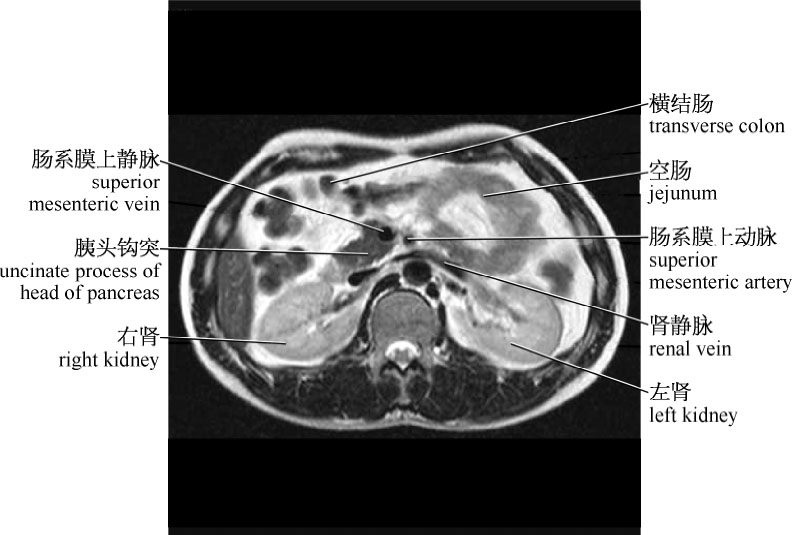
\includegraphics[width=.5\textwidth]{./images/Image00035.jpg}
 \caption{消化道集合淋巴滤泡}
 \label{fig2-10}
  \end{figure} 

\begin{figure}[!htbp]
 \centering
 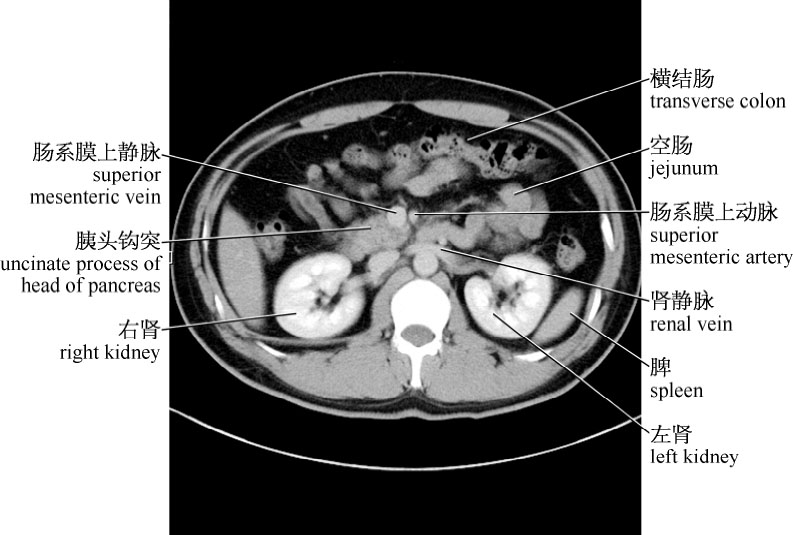
\includegraphics[width=.6\textwidth]{./images/Image00036.jpg}
 \caption{肠道M细胞的转运功能及M细胞包围住大肠杆菌}
 \label{fig2-11}
  \end{figure} 

黏膜免疫系统在保护黏膜表面不受病原体侵害、促进与共生微生物群落共生中都起主要作用。要激发黏膜免疫反应,黏膜表面上的抗原必须首先穿过不可透过的上皮障碍,进入“派伊尔小结”这样的淋巴结构。这一功能(被称为“转胞吞作用”)被认为主要由M细胞调控,它们是“派伊尔小结”中专门的上皮细胞。对由M-细胞调控的抗原“转胞吞作用”的机制所做的一项研究表明,在小肠M细胞顶面表达的糖蛋白-2是表达FimH抗原的细菌的转胞吞受体。由于M-细胞被认为是各种口服免疫药物的一个很有希望的目标,所以这项工作表明,依赖于糖蛋白-2的“转胞吞作用”是一个可能的免疫目标。

3.支气管相关淋巴组织(bronchial-associated
tissue,BALT):主要分布于各肺叶的支气管上皮下,其结构与派氏集合淋巴结相似,滤泡中淋巴细胞受抗原刺激常增生成生发中心,其中主要是B细胞。

(二)MALT的功能及其特点

1.参与局部免疫应答:分布在不同部位的MALT均是参与局部特异性免疫应答的主要场所,从而在消化道、呼吸道和泌尿生殖道的局部免疫防御中发挥关键作用。

2.分泌型IgA(secretory
IgA,SIgA):以消化道黏膜为例,口服抗原被吸收进入集合淋巴结后,可引发B细胞应答,使之转化为产生抗体的浆细胞,其中可分泌SIgA的浆细胞主要定居于集合淋巴结或迁移至固有层。SIgA在抵御病原体侵袭消化道、呼吸道和泌尿生殖道中发挥重要作用。

3.参与口服抗原介导的免疫耐受:口服蛋白抗原刺激黏膜免疫系统后,常可导致免疫耐受,其机制尚未阐明。口服抗原诱导耐受的生物学意义在于:①可阻止机体对肠腔内共栖的正常菌群产生免疫应答,而这些菌群的存在乃正常消化和吸收功能所必需;②通过口服抗原诱导机体对该抗原形成特异性无反应性,可能为治疗自身免疫病提供新途径。

\begin{center}
\textbf{\Large 附:淋巴细胞再循环}
\end{center}

各种免疫器官中的淋巴细胞并不是定居不动的群体,而是通过血液和淋巴液的循环进行有规律的迁移,这种规律性的迁移为淋巴细胞再循环(lymphocyterecirculation)。通过再循环,可以增加淋巴细胞与抗原接触的机会,更有效地激发免疫应答,并不断更新和补充循环池的淋巴细胞。

1.再循环的细胞淋巴干细胞从骨髓迁移至胸腺和腔上囊或其功能器官,分化成熟后进入血液循环的定向移动过程不属于再循环范围。再循环是成熟淋巴细胞通过循环途径实现淋巴细胞不断重新分布的过程。再循环中的细胞多是静止期细胞和记忆细胞,其中80%以上是T细胞。这些细胞最初来源于胸腺和骨髓;成年以后,主要靠外周免疫器官进行补充。受抗原刺激而活化的淋巴细胞很快定居于外周免疫器官,不再参加再循环。

2.再循环的途径血液中的淋巴细胞在流经外周免疫器官(以淋巴结为例)时,在副皮质区与皮质区的连接处穿过高内皮毛细血管后静脉(HEV)进入淋巴结;T细胞定位于副皮质,B细胞主要定位于皮质区;以后均通过淋巴结髓窦迁移至输出淋巴管,进入高一级淋巴结;经过类似的路径,所有外周免疫器官输出的细胞最后都汇集于淋巴导管;身体下部和左上部的汇集到胸导管,从左锁骨下静脉角返回血循环;右侧上部的汇集到右淋巴管,从右锁骨下静脉返回血循环。再循环一周约需24~48小时。

3.细胞定居选择淋巴细胞从血循环进入淋巴组织具有高度的选择性,这是因为淋巴细胞上具有特殊的受体分子,称为归巢受体(homingreceptor)。现已发现的归巢受体包括CD44、LFA-1、VLA-4和MEL-14/LAM-1等;其中MEL-14/LAM-1是定居淋巴结的受体,识别淋巴结内的高内皮细胞;VLA-4的α亚单位是定居MALT的受体,识别黏膜表面的配体。

淋巴细胞再循环的意义:带有不同特异性抗原受体的各种淋巴细胞不断在体内各处巡游,增加了与抗原以及抗原递呈细胞接触的机会;许多免疫记忆细胞也参与淋巴细胞再循环,一旦接触到相应抗原,可立即进入淋巴组织发生增殖反应,产生免疫应答。淋巴细胞再循环如图\ref{fig2-12}所示。

\begin{figure}[!htbp]
 \centering
 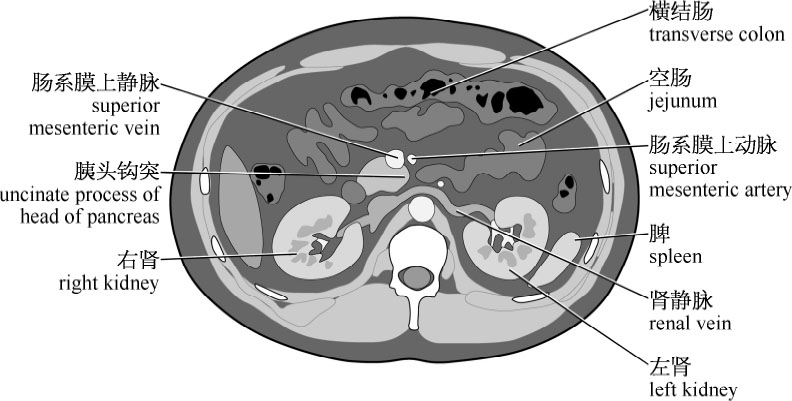
\includegraphics[width=.6\textwidth]{./images/Image00037.jpg}
 \caption{淋巴细胞再循环示意图}
 \label{fig2-12}
  \end{figure} 

\section{免疫细胞}

免疫细胞乃泛指所有参与免疫应答或与免疫应答有关的细胞及其前体,包括造血干细胞、淋巴细胞、专职抗原递呈细胞(树突状细胞、单核-巨噬细胞)及其他抗原递呈细胞、粒细胞、肥大细胞和红细胞等,如图\ref{fig2-13}所示。

\begin{figure}[!htbp]
 \centering
 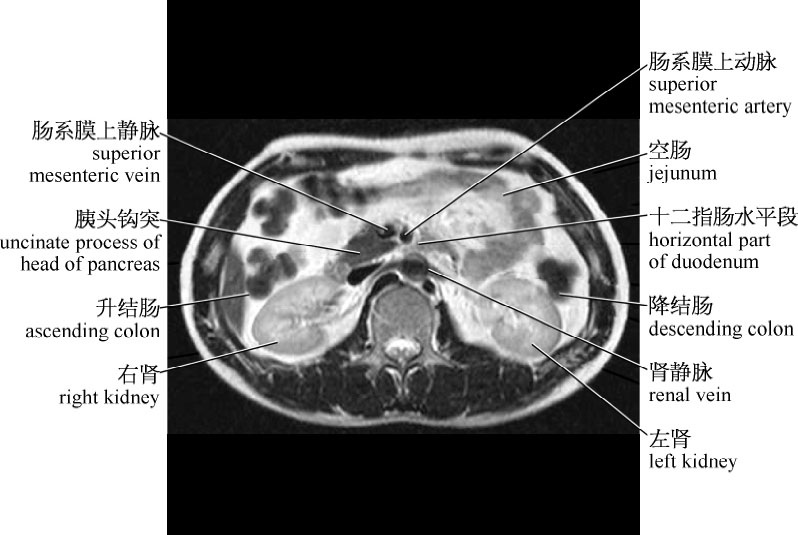
\includegraphics[width=.6\textwidth]{./images/Image00038.jpg}
 \caption{各种免疫细胞}
 \label{fig2-13}
  \end{figure} 


\subsection{造血干细胞}

造血干细胞(hemopoietic stem
cell,HSC)又称多能干细胞,是存在于造血组织中的一群原始造血细胞。也可以说,它是一切血细胞(其中大多数是免疫细胞)的原始细胞。由造血干细胞定向分化、增殖为不同的血细胞系,并进一步生成血细胞。人类造血干细胞首先出现于胚龄第2~3周的卵黄囊,在胚胎早期(第2~3月)迁至肝、脾,第5个月又从肝、脾迁至骨髓。在胚胎末期一直到出生后,骨髓成为造血干细胞的主要来源,具有多潜能性,即具有自身复制和分化两种功能。


\subsection{淋巴细胞}

淋巴细胞(lymphocyte)是构成免疫系统的主要细胞类别,占外周血白细胞总数的20%~45%,成年人体内约有10\textsuperscript{12}
个淋巴细胞。淋巴细胞可分为许多表型与功能均不同的群体,如T细胞、B细胞、NK细胞等;T细胞和B细胞还可进一步分为若干亚群。这些淋巴细胞及其亚群在免疫应答过程中相互协作、相互制约,共同完成对抗原物质的识别、应答和清除,从而维持机体内环境的稳定。

其特点是:未活化淋巴细胞在抗原的刺激下转变为淋巴母细胞,再进一步转变为效应T细胞与记忆细胞。可分群为:
\begin{itemize}
\item T细胞:细胞膜上表达CD3分子和TCR
\item B细胞:细胞膜上表达BCR
\item NK细胞:细胞膜上表达CD56和CD16
\end{itemize}

(一)T淋巴细胞

T淋巴细胞(T
lymphocyte)简称T细胞,其介导细胞免疫应答,并在机体针对TD抗原的体液免疫应答中发挥重要的辅助作用。骨髓中的淋巴样前体细胞(lymphoid
precursor)进入胸腺,经历一系列有序的分化过程,才能发育为成熟T细胞。T细胞乃高度异质性的细胞群,依据其表面标志及功能特征,可分为若干亚群。在免疫应答过程中,各亚群T细胞相互协作,共同发挥重要的免疫学功能。

1.T细胞的表面标志

T细胞表面标志即其膜分子(如图\ref{fig2-14}所示),是T细胞识别抗原、与其他免疫细胞相互作用、接受信号刺激并产生应答的物质基础,亦是鉴别和分离T细胞的重要依据。在诸多表面标志中,TCR、CD3分子是外周血成熟T细胞各亚群的共有标志。

(1)T细胞表面受体(surface antigen):T细胞抗原受体(T cell antigen
receptor,TCR)、细胞因子受体(cytokine receptor,CKR)、丝裂原受体。

(2)T细胞表面抗原(surface antigen):MHC抗原、分化抗原(CD分子)等。

\begin{figure}[!htbp]
 \centering
 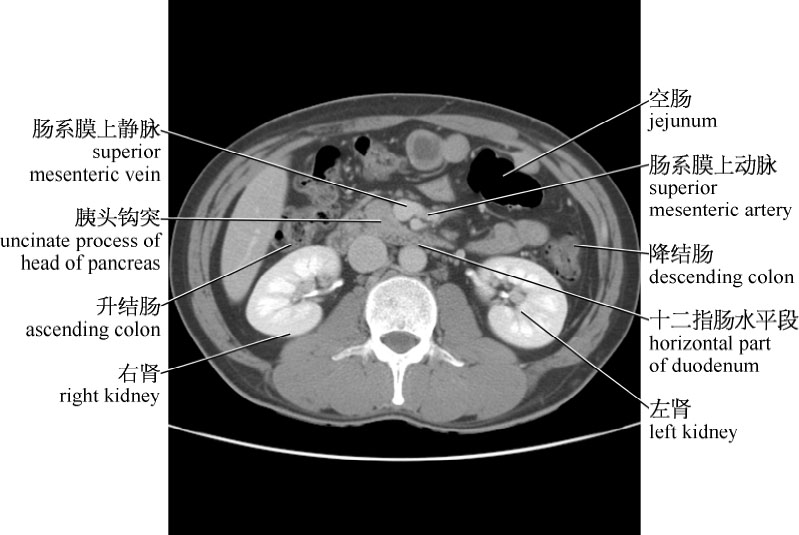
\includegraphics{./images/Image00039.jpg}
 \caption{T细胞表面标志}
 \label{fig2-14}
  \end{figure} 

2.T细胞亚群及其功能

人类的T细胞不是均一的群体,根据表面标志和功能可为五个亚群:

CD4\textsuperscript{+}
T(初始T细胞,Th1细胞,Th2细胞):占T细胞的65\%左右,它的重要标志是表面有CD4抗原。Th细胞能识别抗原,分泌多种淋巴因子,它既能辅助B细胞产生体液免疫应答,又能辅助T细胞产生细胞免疫应答,是扩大免疫应答的主要成分,它还具有某些细胞免疫功能。

CD8\textsuperscript{+}
T(杀伤性T细胞,抑制性T细胞):杀伤性T细胞占T细胞的20%~30%,表面也有CD8抗原。杀伤性T细胞能识别结合在MHC-Ⅰ类抗原上的异抗原,在异抗原的刺激下可增殖形成大量效应性杀伤性T细胞,能特异性地杀伤靶细胞,是细胞免疫应答的主要成分。抑制性T细胞占T细胞的10%左右,表面有CD8抗原。抑制性T细胞常在免疫应答的后期增多,它分泌的抑制因子可减弱或抑制免疫应答。

(1)初始T细胞(naive T
cell):指未完全分化的Th细胞,是Th1、Th2细胞的前体,分泌低水平的IL-4和IFN-γ。

功能:调节体液免疫应答和细胞免疫应答,分化产生Th1、Th2细胞,T细胞的分化如图\ref{fig2-15}所示。

\begin{figure}[!htbp]
 \centering
 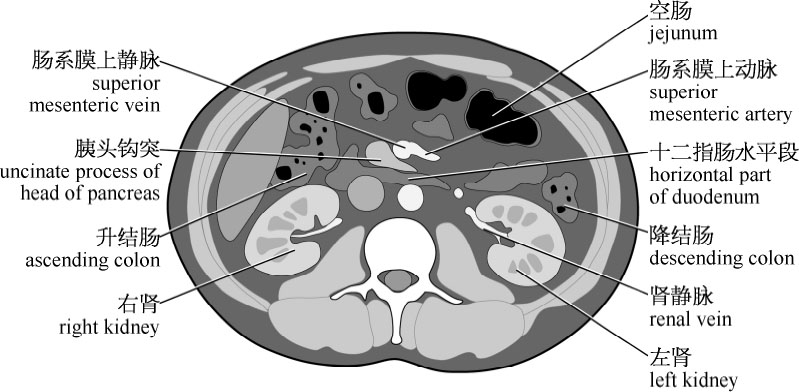
\includegraphics{./images/Image00040.jpg}
 \caption{T细胞的分化}
 \label{fig2-15}
  \end{figure} 

按分泌的细胞因子不同可将Th细胞分为两个不同的亚群:分泌IFN-γ、IL-2的称为TH1细胞,分泌IL-4、IL-5的称为Th2细胞。

(2)Th1细胞:初始T细胞在IL-12作用下转变为Th1细胞。

Th1细胞功能:释放IL-2、IFN-γ和TNF,引起炎症反应或迟发型超敏反应,称为炎症性T细胞。参与细胞免疫应答及迟发型超敏反应。在抗胞内病原微生物等感染中起重要作用。Th1细胞持续性强应答,可能与器官特异性自身免疫病、接触性皮炎、不明原因的慢性炎症性疾病、迟发型超敏反应性疾病、急性同种异体移植排斥反应等的发生有关。

(3)Th2细胞:初始T细胞在IL-4作用下转变为Th2细胞。

释放IL-4、5、6、10,诱导B细胞增殖分化、合成并分泌抗体,引起体液免疫应答或速发型超敏反应(图\ref{fig2-16})。

\begin{figure}[!htbp]
 \centering
 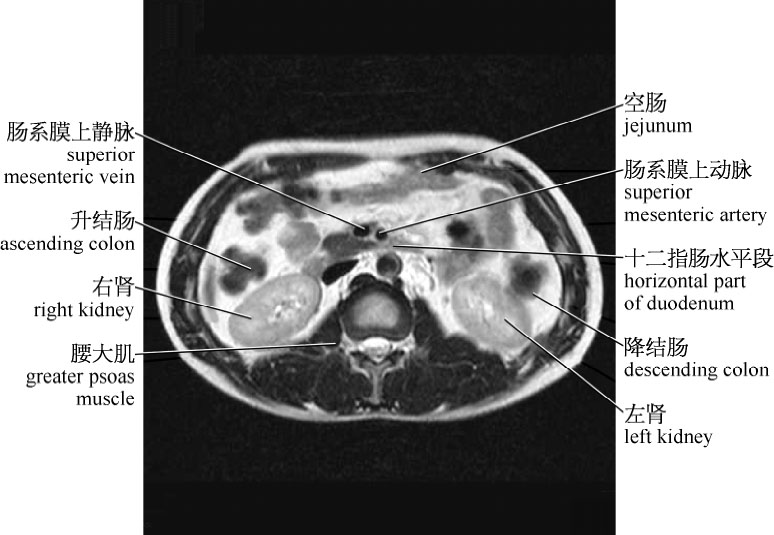
\includegraphics[width=.5\textwidth]{./images/Image00041.jpg}
 \caption{Th1、Th2淋巴细胞的功能}
 \label{fig2-16}
  \end{figure} 

(4)杀伤性T细胞(CTL):也叫细胞毒性T细胞,是效应T细胞,经抗原致敏后,CTL
的TCR特异性识别靶细胞(如病毒感染细胞、肿瘤细胞、同种异体移植物细胞等)表面的抗原肽/MHC-I类分子复合物。活化CTL
杀伤效应的主要机制为:①分泌穿孔素(perforin)、颗粒酶(granzyme)或淋巴毒素等直接杀伤靶细胞;②通过高表达FasL导致Fas阳性的靶细胞凋亡。CTL参与的免疫效应为抗病毒感染、抗肿瘤和介导同种异体移植排斥反应等(图\ref{fig2-17})。

\begin{figure}[!htbp]
 \centering
 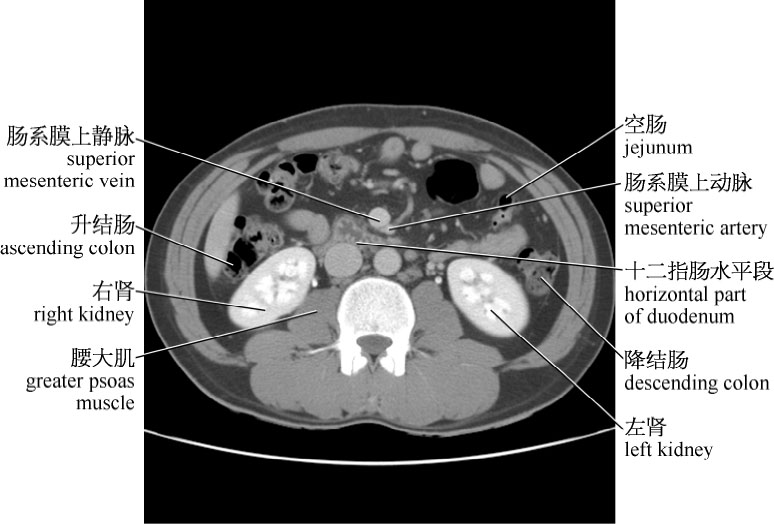
\includegraphics[width=.5\textwidth]{./images/Image00042.jpg}
 \caption{CTL的免疫效应}
 \label{fig2-17}
  \end{figure} 

(5)Ts细胞(suppressor T cell,Ts):具有抑制体液免疫和细胞免疫的功能。

(二)B淋巴细胞

B淋巴细胞(B
lymphocyte)是始祖B淋巴细胞在骨髓(人、动物)、法氏囊(禽)中发育、分化、成熟,产生抗体,也称骨髓或囊依赖性细胞,是体内唯一能产生抗体(Ig)的细胞,主要执行体液免疫,也具有抗原递呈功能。外周血中占淋巴细胞总数10\%~15\%,简称B细胞,是由哺乳动物骨髓或鸟类法氏囊中的淋巴样前体细胞分化成熟而来。

1.B细胞的表面标志

B细胞表面标志如图\ref{fig2-18}所示。

\begin{figure}[!htbp]
 \centering
 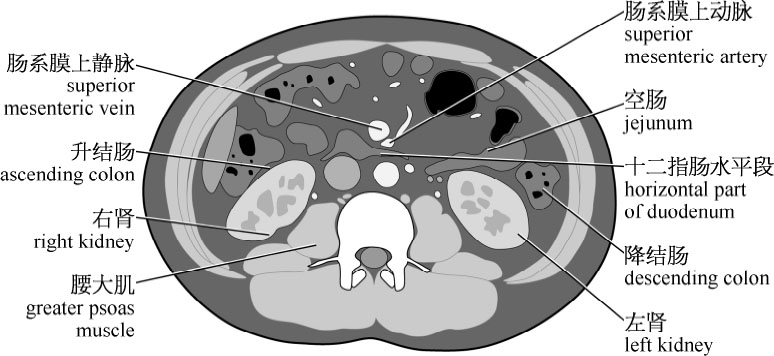
\includegraphics[width=.5\textwidth]{./images/Image00043.jpg}
 \caption{B细胞表面标志}
 \label{fig2-18}
  \end{figure} 

(1)B细胞抗原受体(B-cell antigen
receptor,BCR):BCR是嵌入细胞膜类脂分子中的膜表面免疫球蛋白(mIg),乃B细胞的特征性表面标志,也是B细胞特异性识别不同抗原表位的分子基础。

(2)细胞因子受体:B细胞表面表达IL-1R、IL-2R、IL-4R、IL-5R、IL-6R、IL-7R及IFN-γR等多种细胞因子受体。细胞因子通过与B细胞表面相应受体结合而参与或调节B细胞活化、增殖和分化。

(3)补体受体(CR):多数B细胞表面表达CR1和CR2(即CD35和CD21)。CR1主要见于成熟B细胞,其在B细胞活化后表达增高。CR1与相应配体结合可促进B细胞活化。CR2(CD21)是EB病毒受体,在体外应用EB病毒感染B细胞可使之转化为B淋巴母细胞系,从而达到永生化(immortalized)。

(4)Fc受体:多数B细胞表达IgG Fc受体Ⅱ(FcγRⅡ),可与免疫复合物中的IgG
Fc段结合,有利于B细胞捕获和结合抗原,并促进B细胞活化和抗体产生。

(5)丝裂原受体:某些丝裂原通过与B细胞表面相应受体结合,使其被激活并增殖分化为淋巴母细胞,可用于检测B细胞功能状态。美洲商陆(PWM)对T细胞和B细胞均有致有丝分裂作用;脂多糖(LPS)是常用的小鼠B细胞丝裂原。

2.细胞表面抗原

(1)MHC抗原:B细胞可表达MHC-Ⅰ类和MHC-Ⅱ类抗原。MHC-Ⅱ类抗原可与Th细胞表面CD4结合,增强B细胞与Th细胞间的黏附作用,并参与抗原递呈和淋巴细胞激活。

(2)CD抗原:B细胞分化发育的不同阶段,其CD抗原的表达各异,有CD19、CD20、CD21、CD40/CD40L、CD80(B7-1)/CD86(B7-2)。

3.B细胞亚群及功能

根据是否表达CD5分子,可将人B细胞分为B1(CD\textsuperscript{+}
\textsubscript{5} )和B2(CD\textsuperscript{-} \textsubscript{5}
)细胞。

(1)B1细胞亚群:B1细胞在个体发育过程中出现较早,是由胚胎期或出生后早期的前体细胞分化而来,其发生不依赖于骨髓细胞。B1细胞产生后,成为具有自我更新(self-renewal)能力的长寿细胞,主要分布于胸腔、腹腔和肠壁固有层中。B1细胞的抗原识别谱较窄,主要针对属于TI-2抗原的多糖类物质,尤其是某些菌体表面共有的多糖抗原(如肺炎球菌荚膜多糖等)。B1细胞的功能特点是:主要产生IgM类的低亲和力抗体;不发生抗体类别转换;无免疫记忆。

(2)B2细胞亚群:B2细胞即通常所称的B细胞,是参与体液免疫应答的主要细胞类别。它是由骨髓中多能造血干细胞分化而来,属形态较小、比较成熟的B细胞,在体内出现较晚,定位于外周淋巴器官。B2细胞的主要生物学功能为:参与体液免疫应答、抗原递呈、免疫调节。

(三)自然杀伤细胞

自然杀伤细胞(natural
killer,NK)是一类独立的淋巴细胞群,其不同于T细胞和B细胞,不表达特异性抗原识别受体(图\ref{fig2-19})。NK细胞胞浆内有许多嗜苯胺颗粒,故又称为大颗粒淋巴细胞(large
granular
lymphocyte)。NK细胞无须抗原预先致敏即可直接杀伤某些靶细胞,包括肿瘤细胞、病毒或细菌感染的细胞以及机体某些正常细胞(图\ref{fig2-20})。
\begin{figure}[!htbp]
    \centering
    \begin{minipage}[b]{0.45\textwidth} 
      \centering
        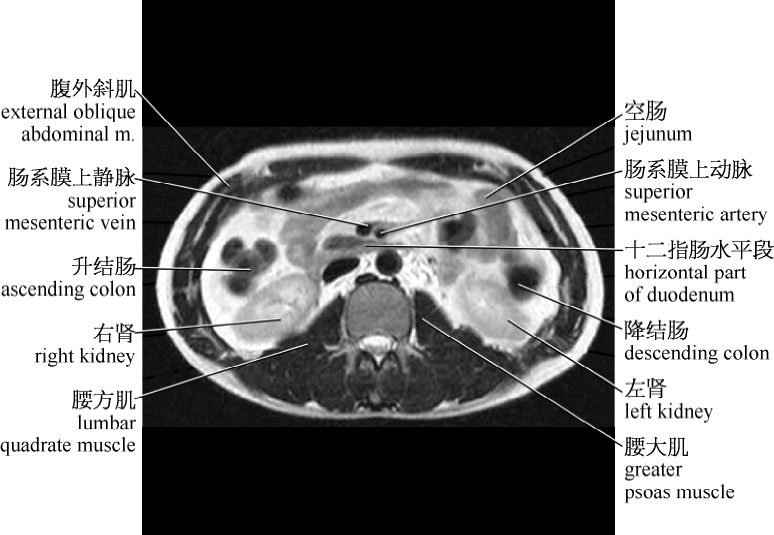
\includegraphics[height=0.12\textheight]{./images/Image00044.jpg}
        \captionsetup{justification=centering}
        \caption{自然杀伤细胞}
        \label{fig2-19}
    \end{minipage}
%	\end{figure} 
	%\FloatBarrier
%\begin{figure}[!htbp]
%    \centering
%\hspace{0.04\textwidth}%
\begin{minipage}[b]{0.45\textwidth} 
  \centering
    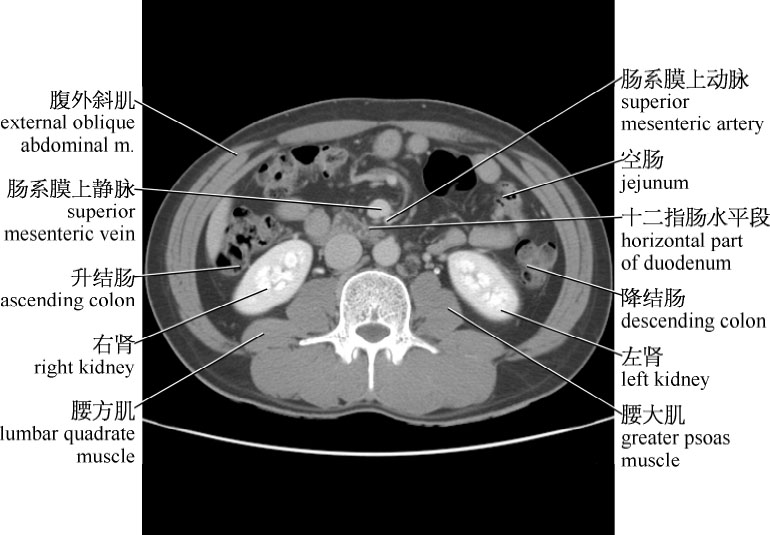
\includegraphics[height=0.2\textheight]{./images/Image00045.jpg}
    \captionsetup{justification=centering}
    \caption{NK细胞杀死癌细胞}
    \label{fig2-20}
\end{minipage}
\end{figure} 

1.来源及分布

NK细胞是由骨髓中的共同淋巴样祖细胞(commen lymphoid
progenitor,CLP)分化而来,其发育、成熟可能循骨髓途径或胸腺途径。人类和小鼠NK细胞主要分布于脾脏(占脾细胞总数3\%~4\%)和外周血(占淋巴细胞总数5%~7%),在淋巴结以及其他组织内(如肺脏等)也有少量NK细胞存在。近年发现,肝脏中NK细胞占淋巴细胞总数50\%以上,其生物学意义有待阐明。

2.功能

(1)能非特异性杀伤某些肿瘤细胞和病毒感染的靶细胞,具有抗肿瘤、抗感染的功能。

(2)NK细胞可产生IL-1、IFN-r、TNF等,有免疫调节作用。

(3)参与移植排斥反应、自身免疫病、超敏反应的发生。


\subsection{单核吞噬细胞系统}

单核吞噬细胞系统(mononuclear phagovyte
system,MPS)包括单核细胞、巨噬细胞,是体内具有最活跃生物学功能的细胞类型之一(图\ref{fig2-21})。

\begin{figure}[!htbp]
 \centering
 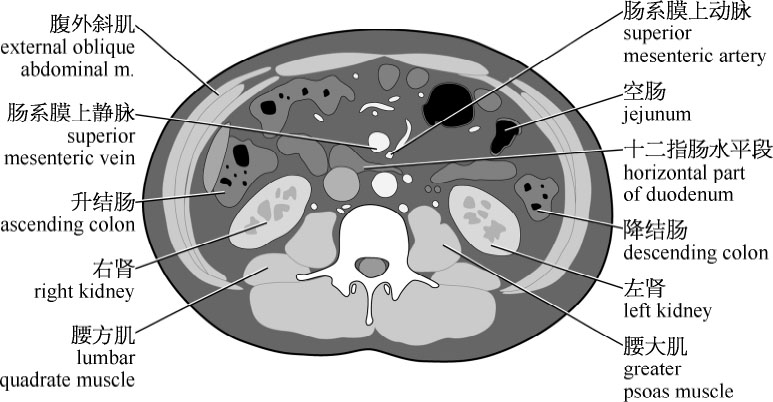
\includegraphics[width=.7\textwidth]{./images/Image00046.jpg}
 \caption{单核吞噬细胞}
 \label{fig2-21}
  \end{figure} 

1.表面标志:表达多种表面标志,并借此发挥各种生物学功能,如MHC分子、黏附分子等。这些表面标志不仅参与细胞黏附及对颗粒抗原的摄取、递呈,也介导相应配体触发的跨膜信号转导,并影响细胞分化和发育等。

2.产生多种酶及分泌产物:单核吞噬细胞能产生各种溶酶体酶、溶菌酶、髓过氧化物酶等,还能产生和分泌近百种生物活性物质,如细胞因子(IL-1、IL-6、IL-12等)、补体成分(C1、P因子等)、凝血因子,以及前列腺素、白三烯、血小板活化因子、ACTH、内啡肽等活性产物。

3.功能:具有抗感染、抗肿瘤、免疫调节的作用。


\subsection{其他免疫细胞}

(一)中性粒细胞

中性粒细胞表面具有IgFc受体和C3b受体,具有高度趋化性和非特异性功能,有抗感染作用(图\ref{fig2-22})。

\begin{figure}[!htbp]
 \centering
 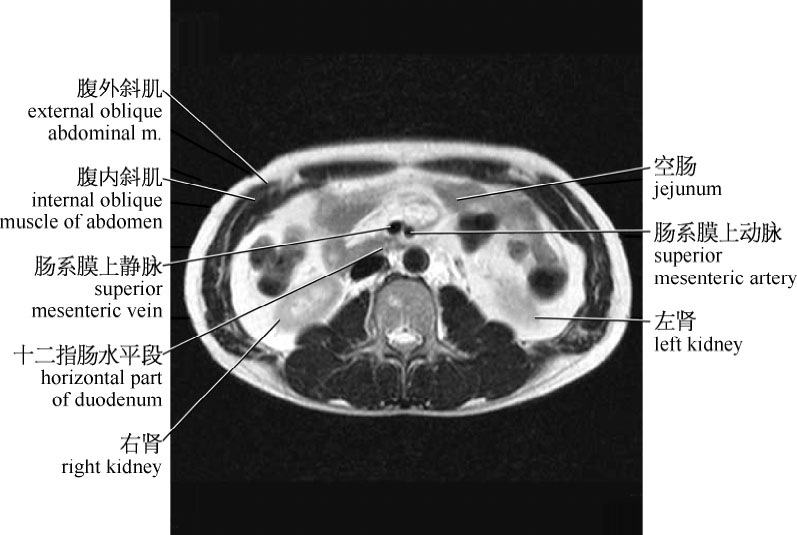
\includegraphics[width=.7\textwidth]{./images/Image00047.jpg}
 \caption{中性粒细胞的吞噬作用}
 \label{fig2-22}
  \end{figure} 

(二)嗜酸性粒细胞

嗜酸性粒细胞具有IgFc受体,参与IgE介导的ADCC效应;具有吞噬作用,抗寄生虫和对I型超敏反应的负调节作用。

(三)嗜碱性粒细胞与肥大细胞

嗜碱性粒细胞与肥大细胞表面具有IgE的Fc受体,能参与I型超敏反应、抗肿瘤作用(图\ref{fig2-23})。

\begin{figure}[!htbp]
 \centering
 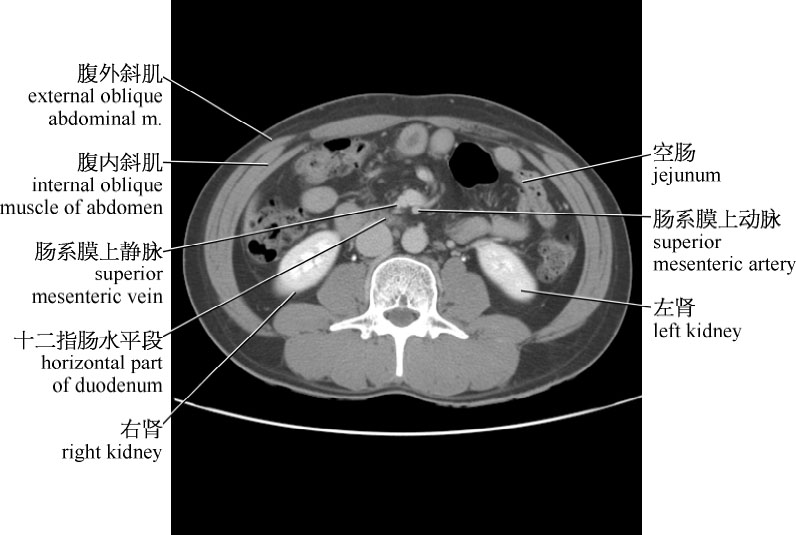
\includegraphics[width=.6\textwidth]{./images/Image00048.jpg}
 \caption{肥大细胞参与Ⅰ型超敏反应}
 \label{fig2-23}
  \end{figure} 

(四)红细胞

1.红细胞免疫的物质基础

① 红细胞CR1分子------结合C3b/C4b;

② 红细胞CD58分子------即LFA-3,与CD2互为配体和受体;

③ 红细胞CD59分子------阻止C9与C5B678结合,促进T细胞有丝分裂;

④ 红细胞CD55分子------即衰变加速因子DAF;

⑤ 红细胞CD44分子------参与T、B的分化、成熟、活化,细胞黏附;

⑥ 红细胞NK细胞增强因子------增强NK细胞的毒性;

⑦ 红细胞趋化因子受体------参与调控炎症反应。

2.红细胞在整体免疫反应中的作用

① 增强吞噬作用;

② 清除循环免疫复合物;

③ 识别和携带抗原;

④ 免疫调节作用;

⑤ 效应细胞的作用。

\section{思考练习与课外阅读}
\noindent\textbf{【理解与思考】}

1.你能向一位没有免疫学知识的人,形象地解说机体免疫系统的构成及其作用吗?

2.你能描绘出体内淋巴细胞的一生历程吗?

3.如果你是一病原微生物,进入机体后你能遭遇哪些危险?

4.如果你是一免疫细胞,你又是如何保证机体健康的?

5.以红细胞的口气,向别人叙述一下你在人体内的贡献。

\noindent\textbf{【课外拓展】}

1.白血病中,为何某一种白细胞数量过度增加?其分化机理如何?

2.淋巴细胞的阴性选择、阳性选择是如何进行的?有何意义?

3.造血干细胞的分化过程如何?在哪些因素作用下发生的?

4.与红细胞等比较,为何白细胞类都是“短命细胞”?

5.自然杀伤细胞在肿瘤防治中有哪些作用?目前用免疫的方法治疗肿瘤有哪些方法?

\noindent\textbf{【课程实验与研究】}

1.设计一个检测淋巴细胞活性的实验。要求分类定量。

2.设计一种诱导造血干细胞分化为NK细胞的实验方法。

3.白血病的种类有哪些?设计一种通过阻断细胞的分化途径来预防某种类型的白血病方案,并分析可行性。

4.设计一种方案,检测免疫细胞能释放哪些生物活性物质,并实施实验,完成实验报告。

5.设计检测饲喂蜂蜜对小鼠机体免疫力影响的三种以上指标,并设计实验方案,完成实验,写出小论文。

6.Nature最近报道发现“自然杀伤(NK)细胞的一个新亚类”,请问如何鉴别其为新的发现?

\noindent\textbf{【课程研讨】}

1.为何机体免疫细胞对自身的成分不产生排斥?

2.整个免疫系统与一个国家的防御力量有什么相似之处?请加以比较说明。

3.免疫系统与机体别的系统一样,各自负起使命,你认为机体是如何抵御病原微生物入侵的?如果病原微生物进入机体,机体又是如何清除的?

4.如何区别不同的淋巴细胞?

5.查阅资料,阐述淋巴细胞当今的研究进展。

\noindent\textbf{【课后思考】}

1.详细叙述免疫系统的构成及其作用。

2.骨髓、胸腺、淋巴结、脾脏的主要免疫功能。

3.T、B淋巴细胞的分类及其作用。

\noindent\textbf{【课外阅读】}

\begin{center}
\textbf{\Large 红细胞免疫发展史}
\end{center}

红细胞免疫和其他自然科学一样,它的发展也经历着三个阶段,即经验、实验、理论阶段。在发展中各阶段难以截然分开,反复循环,不断深入,不断提高。

\begin{center}
{\large 一、经验阶段}
\end{center}

我国劳动人民在长期与疾病的斗争中体会到血液的重要,往往将血与生命联系在一起,事实上血液特别是红细胞是机体生命活动的物质基础。祖国医学云:“气血是人体生命活动的物质基础”,“离开了气血,则整体不能联系,人身无有依附”。在20世纪初,Landsteiner
用免疫学方法在人类红细胞与血液混合实验中,观察到凝聚现象,后来通过多次反复试验观察,发现了人类ABO
血型系统,认识了红细胞表面存在许多能与血清中相应抗体凝集的抗原,如Mn、P
型、Rn、Lutheran、Lewis、Kell、Duffy、Kidd
等。除目前已知的数十种血型抗原外,发现红细胞还含有其他抗原。20世纪30年代,杜克(L
.H.Duke)首先发现锥虫在抗血清及补体存在时可黏附到人类红细胞上,推测在人的红细胞膜上存在有一种与免疫有关的物质。在临床上,人们对某些疑难病、原因不明性疾病等患者,采用输新鲜血液的办法,往往可得到满意的治疗效果。但究其原因,过去人们并不很清楚,自红细胞免疫问世以来,人们对上述现象的解释有了理论依据。如
G-BS
现已证实属红细胞免疫缺陷症;有些疾病,由于输注红细胞后,机体免疫功能得到了改善,即给了机体以
“气血”,“气血相依,循环不已”,“防治百病莫不以气血为本”。

\begin{center}
{\large 二、实验阶段}
\end{center}

实验阶段即将人们观察到的现象,进行科学实验的过程。1953年,R.A.Nelson用正常人的红细胞、白细胞与相应抗体致敏的
I
型肺炎双球菌进行培养,发现肺炎双球菌可黏附于正常人的红细胞表面并被白细胞吞噬,其吞噬率可达60\%,远远高于未加相应抗体组和未加相应红细胞组,作者推测红细胞膜存在免疫黏附受体,将此命名为免疫黏附现象。1963年,Nishioka证实红细胞这种免疫黏附现象是通过红细胞膜
C3受体实现的。1980年,Fearon从红细胞膜分离到这一受体,并详细研究了CR1的性质,是分子量190
000~250
000的多态性膜糖蛋白。1986年,郭峰通过体外对比实验证明红细胞可黏附补体调理过的各种肿瘤细胞,并发现红细胞可黏附未经调理过的肿瘤细胞,其机理不明。1992年,刘景田等证实这种直接免疫黏附的机理与红细胞上
CR1 和肿瘤细胞上 C3b分子有关。

\begin{center}
{\large 三、理论阶段}
\end{center}

1981年,美国生殖免疫学家Siegel在前人研究的基础上发现红细胞有多种免疫功能,红细胞可黏附胸腺细胞,并发现血清中存在有红细胞免疫黏附抑制因子,预见了血清中存在有红细胞免疫调节系统,推测红细胞在阻止肿瘤细胞血行转移中有作用。他综合看待以往对红细胞免疫的研究成果,提出了
“红细胞免疫系统” 的新概念,冲破了传统上划分血细胞功能的
“界限”,更新了人们对红细胞功能的认识。20 世纪 80
年代,我国学者郭峰教授在红细胞免疫的基础理论和应用研究方面取得了许多突破性进展,如发现血清中存在有红细胞免疫黏附促进因子、红细胞有增强各类免疫细胞的免疫功能,建立了许多红细胞免疫功能的监测方法等,大大推动了我国红细胞免疫的发展。1994
年,刘景田在证实血清中确实存在有正负两种红细胞调节因子的基础上,发现了这两种因子对粒细胞、淋巴细胞(主要指B
淋巴细胞)都有相同调节作用,推测这种因子对具有
CR1的细胞都有调节作用,故将这种因子称为 CR1 免疫调节因子(Complement
recepor 1 immuneregalation factors,CR1FR)。其中具有正调节作用者称为
CR1免疫黏附促进因子(Complement recepor 1 immune regalation enhance
factors,CR1FER);具有负调节作用者称为 CR1 免疫黏附抑制因子(Complement
recepor 1 immune regalation inhibitor factors,CR1FIR)。

(资料来源:刘景田,党小军.红细胞作为免疫细胞的事实及意义[J].深圳中西医结合杂志,2002,12(1):10-12)

\begin{center}
\textbf{\Large 红细胞免疫功能研究进展}
\end{center}

红细胞是血液中最主要的细胞成分。传统认为,红细胞结构简单,功能单一,仅运输氧和二氧化碳。随着科技的发展,人们对红细胞免疫功能的认识不断深入。1930年,Duck发现人类红细胞膜上存在与免疫有关的物质;1953年,Nelson首次提出红细胞不仅具有免疫黏附功能还能促进白细胞的吞噬作用;1963年,Nishioka证实红细胞免疫黏附的物质基础是红细胞膜上补体C3b受体(C3breceptor,C3bR);1980年,Fearon进一步从红细胞膜上分离出受体CR1(complementreceptor1,CR1)。1981年,Siegel在前人研究的基础上提出了“红细胞免疫系统(redcellimmunesystem,RCIS)”新概念,成为红细胞免疫研究的里程碑,促进了红细胞免疫研究工作的迅速发展。医学工作者研究发现,红细胞具有很多与免疫有关的物质,包括补体受体CR1、CR3、淋巴细胞功能相关抗原-3(CD58)、CD44、人类补体膜辅助因子蛋白(MCP)、降解加速因子(DAF)、过氧化物歧化酶(SOD)、阿片肽受体、NK细胞激活因子(NKAF)以及红细胞趋化因子受体等。红细胞不仅具有识别、存储、递呈抗原,清除免疫复合物,促进吞噬细胞功能等作用,自身还存在完整的自我调节控制系统,是机体免疫系统的重要组成部分。

\begin{center}
{\large 一、红细胞免疫功能的分子学基础}
\end{center}

1981年,Siegel提出了“红细胞免疫系统”概念,并指出红细胞免疫黏附(redcellimmuneadhesion,RCIA)是红细胞发挥免疫功能的主要手段,RCIA的分子基础则是红细胞膜上的补体受体(complementreceptor,CR)。目前,已明确红细胞膜上的补体受体有I型(CR1)和Ⅲ型(CR3),主要为CR1,其基因结构、分子结构及生物学功能已部分明确。CR1属于补体调控蛋白,分子量为160~260kd,是一种单链膜结合蛋白,能与补体系统中C3b、C4b高亲和性地结合。就单个红细胞而言,膜上CR1受体密度仅为白细胞110~150,但红细胞数量庞大,在体内约90\%C3b受体存在于红细胞膜上。CR1与血液循环中带有C3b的免疫复合物(immnunecomplex,IC)结合,并运送至肝脏及脾脏内皮系统予以清除,即为红细胞免疫黏附(RCIA)机制。随着国内外研究的深入,发现CR1参与机体免疫功能的机制远比上述复杂得多。红细胞能携带抗原抗体复合物,还能主动地将抗原抗体复合物传递给单核巨噬细胞并使之激活,增强单核巨噬细胞对抗原抗体复合物的摄取并加工递呈给T细胞。此外红细胞在类孢子病、溶血性贫血、病毒性肝炎、系统性红斑狼疮、肾病、疟疾等疾病中的作用也得到证实。红细胞上CR1表达降低或红细胞黏附功能下降会引起机体免疫功能低下,研究红细胞CR1介导的免疫黏附功能对评价机体天然免疫功能状况乃至特异性细胞或体液免疫可能都具有十分重要的意义。目前,CR应用热点是对双特异性单抗异聚体(heteropolymer,HP)的研究。Taylor以红细胞CR1分子为桥梁,建立了抗CR1单抗与抗致病原单抗交叉连接的HP清除循环中致病原的方法,引起了广泛关注。HP结合红细胞时,还可结合循环中病原体,形成异聚体复合物(E-HP-Ag),并迅速将EHPAg移至肝脏彻底销毁,红细胞本身数量却无减少。此外可溶性CR的应用也有所突破,Yazdanhakhsh等报道使用基因重组的可溶性CR1在动物实验中成功阻断了补体活化。

\begin{center}
{\large 二、红细胞免疫功能}
\end{center}

(一)清除循环免疫复合物

研究表明,红细胞膜上补体受体具有免疫黏附、携带及清除循环液相中抗原异物的功能,清除循环免疫复合物(circleimmunecomplex,CIC)是红细胞主要的免疫功能。目前认为,大多数C3b-免疫复合物(C3b-IC)通过CR1连接。CR1存在于红细胞、多形核白细胞、巨噬细胞及淋巴细胞的膜表面。红细胞膜上CR1分布有两种形式:散在和集簇分布。约50\%红细胞膜上CR1呈集簇分布,多形核白细胞上CR1集簇分布率小于15\%。CR1集簇分布方式使它与C3b-IC的结合位点呈多价性,连接更牢固。实验证明,单个白细胞表面CR1受体较红细胞多,但在细胞浓度相同时,两种细胞的免疫复合物结合率相同。血液中红细胞总数远远超过白细胞,循环系统中约95\%C3b受体位于红细胞上,与CIC结合机会为白细胞的500~1000倍。因此,体内清除CIC起主要作用的是红细胞,不是白细胞。Nedaf体外实验结果证明了这一推测。红细胞清除免疫复合物的机理是:红细胞通过表面CR1受体与循环中C3b-IC结合(即发生黏附),形成的复合物被血流带到肝、脾等器官,这些器官的固定吞噬系统捕获红细胞结合的IC,通过巨噬细胞膜表面的Fc受体与IC中的抗体Fc段结合,此时红细胞从IC上解离,再度进入循环,而捕获IC的巨噬细胞则通过膜表面CR1受体再与IC补体C3b结合,Fc受体与CR1受体的协同作用使巨噬细胞的吞噬作用加强,而将IC吞噬并清除到体外。Sherwood实验研究发现:红细胞表面所黏附的循环免疫复合物被转运到吞噬细胞,吞噬细胞所接受CIC的多少与红细胞CIC的浓度呈平行关系,红细胞无任何损伤或被吞噬。有实验证明,肝脏内巨噬细胞表面的Fc受体和CR1受体密度较高,且Fc受体比红细胞膜上CR1受体活性强,致使肝、脾内巨噬细胞对免疫复合物(IC)有更强的作用,可以从CR1密度低的红细胞上夺取IC。

(二)增强吞噬细胞的吞噬功能

1953年,Nelson将经抗体、补体调理过的肺类球菌复合物注入猴体,发现球菌几乎全部黏附于红细胞上。实验证明,血浆中被红细胞黏附的复合物(IC)较未被黏附的更容易被吞噬。1982年,Forslod进一步证实了上述现象作用机理,用C3b及IgG(兔抗酵母菌IgG)调理过的酵母菌与吞噬细胞一起孵育,加入红细胞后,吞噬细胞对酵母菌的吞噬率比未加入红细胞组增加了34\%;给予红细胞溶解产物后,吞噬率增加75\%。用过氧化氢酶及超氧化物歧化酶代替红细胞后,吞噬率增加程度相似。可能是红细胞首先黏附酵母菌,然后红细胞酵母菌复合物与吞噬细胞作用,红细胞内含有高浓度的过氧化氢酶(Cat)及超氧化物歧化酶(SOD),并具有强力的抗氧化作用,清除吞噬过程中产生的氧化代谢产物(ROM),促进吞噬作用。近年来,人们将红细胞作为SOD的载体以延长其在体内的存活时间,提高血液相容性,防治缺氧、缺血过程中活性氧造成的组织损伤,取得了良好的效果。

(三)对T淋巴细胞和淋巴因子的调控作用

实验表明,红细胞通过CD58、CD59与T辅助细胞CD2的黏附激活T淋巴细胞免疫功能,与B细胞作用亦能促使增殖、分化产生免疫球蛋白。红细胞还可调控淋巴细胞产生γ-干扰素,增加淋巴细胞转化率和培养液中IgG、IgA的含量。CD58分子即淋巴细胞功能相关抗原23(LFA-3),是一种分子量为55~70kd的糖蛋白,属于免疫球蛋白超家族成员,广泛表达于人体内各种免疫细胞和红细胞上,结构与CD2(LFA-2)相似,故CD58与CD2分子可以相互结合。表达CD58抗原递呈细胞(APC)或靶细胞通过与表达CD2分子的T细胞相互黏附,促进T细胞识别抗原,CD58与CD2结合后又参与细胞信号转导,此信号为T细胞活化的一种重要协同(辅助)刺激信号。相对于T细胞活化时TCR识别性结合MHC一抗原肽复合物的T细胞活化第一信号,CD58与CD2的结合又被称为T细胞活化第二信号。有证据表明,结合抗原抗体复合物(IC)的红细胞通过膜表面CR分子介导的免疫黏附作用将免疫复合物传递给巨噬细胞,又经膜表面CD58分子与辅助性T细胞膜表面CD2分子结合间接起到类似于抗原递呈细胞(antigenpresentingcell,APC)的递呈抗原作用,促进外周血T细胞活化与细胞周期改变,从而间接调控免疫应答。CD59分子即攻膜复合体(membraneattackcomplex,MAC)抑制物,是一种分子量为18~20kd的糖蛋白。CD59可阻碍C7、C8与C5b~6复合物结合,抑制MAC形成。CD59除广泛参与补体调节,还能与CD2分子结合,是继CD58之后发现的又一CD2配体。CD59与CD2结合也能发挥类似CD58与CD2结合的协同刺激信号的作用,CD58和CD59与T细胞黏附时具有协同作用,同时表达CD58与CD59的靶细胞更有利于T细胞的激活。近年来的研究发现,CD59缺陷还常伴随CD55缺陷,提示其功能可能为一种广泛参与红细胞免疫调节的协同蛋白。

(四)识别、储存和递呈抗原

红细胞对自我和非我抗原具有识别功能,且具有储存抗原的能力。1982年Garvey将\textsuperscript{3}
H标记的牛血清清蛋白(BSA)注入新生兔,放射自显影发现外周血液和肝血管内红细胞表面均黏附有\textsuperscript{3}
HBSA,并持续存在4~6周以上。若将兔血清清蛋白注入新生兔体内,则不出现上述现象,由此证实了上述观点。红细胞的抗原递呈能力表现为红细胞免疫黏附特性具有双重性,即红细胞上CR1与IC相黏附时,可同时黏附自身胸腺细胞和T细胞,形成自身玫瑰花环,IC中抗原与T淋巴细胞紧密靠拢,红细胞将抗原递呈给T淋巴细胞,使其俘获抗原能力增强,从而增强了免疫应答。

(资料来源:夏佐中.红细胞免疫功能研究进展[J].重庆医学,2008,37(20):2365-2367)

\begin{center}
\textbf{\Large 天然免疫反应需要T细胞参与}
\end{center}

先天性免疫和获得性免疫虽是不同的概念,具有不同机制,但在对付入侵的病原体时,它们并不各自为政或分庭抗礼,而是互相配合协同作战的。例如,当伤寒杆菌侵入后,首先由先天性免疫(如补体、吞噬细胞等)对付,等到体内产生抗伤寒抗体和免疫淋巴细胞(获得性免疫因素),就与补体和吞噬细胞(先天免疫因素)协同作用,清除体内伤寒杆菌。

2009年1月,中科院生物物理所感染免疫中心唐宏研究员和傅阳心教授在《免疫学趋势》(Trends
in Immunology)杂志上以《Do adaptive immune cells suppress or activate
innate
immunity》为题,系统阐述了他们近来提出的“天然免疫反应需要T细胞参与”的新理论。经典的免疫学理论认为,天然免疫反应启动获得性免疫,而获得性免疫随后进一步放大天然免疫效应,二者的合作与平衡才能清除入侵病原,起到免疫保护的作用。该实验室近期的研究结果表明(原文见Nature
Medicine,2007;Nature Reviews in Immunology,2007; Nature
China,2008),原先关于区分天然免疫和获得性免疫的界限可能并不那么清楚,T细胞其实也参与天然免疫反应并维持其稳态。经典理论认为天然免疫和获得性免疫反应的双重低下是早产儿容易死于急性感染的主要原因。该实验室的研究发现,实际上,在感染早期获得性免疫细胞对于天然免疫反应具有负调控的作用,从而有效地将天然免疫反应的强度控制在一定的水平内而不至于对机体造成免疫损伤。新生鼠或早产儿由于获得性免疫低下,天然免疫炎性反应无法得到有效控制,这种“炎性因子风暴”才是致死原因。因此,获得性免疫一方面抑制感染早期的炎症反应,另一方面在感染后期行使病原特异性清除功能,两者缺一不可。

这个新理论对于深入了解病毒性感染的炎症反应和病毒清除机理,控制免疫低下病人(新生儿、老年人、放化疗癌症病人、器官移植患者或艾滋病人)机会性感染具有极高的指导价值。

(资料来源:http://www.bioon.com/biology/Immunology/383575.shtml)

\begin{center}
\textbf{\Large Immunity:嗜中性粒细胞通过群集抵抗寄生物}
\end{center}

嗜中性粒细胞在抵抗病原体的免疫响应中扮演了一个重要角色,但是它们调节自身保护效应的机制却一直没有搞清。最近发表在《免疫学》上的一项研究显示,在嗜中性粒细胞转移到淋巴结的过程中------它们在这里形成了动态分子团,就像蜂群一样,这些细胞扮演了抵抗胞内寄生物的一个重要角色。

为了研究嗜中性粒细胞与淋巴结之间的关系,美国加利福尼亚大学伯克利分校的Tatyana
Chtanova等使用了嗜中性粒细胞表达绿色荧光蛋白质的小鼠,并使它们传染上胞内寄生物------弓形虫,同时利用荧光显微镜方法检测淋巴结组织切片。研究人员观察到,在感染后,嗜中性粒细胞迅速转移到淋巴结中,并且这一过程依赖于它们的适应物蛋白质MyD88(骨髓差别主要响应基因88)的表达。此外,渗透的嗜中性粒细胞被发现形成了群集,并且这些群集与寄生虫在淋巴结中所处的位置相符合。

利用完整无损的淋巴结的双光子激光扫描显微镜,研究人员随后调查了嗜中性粒细胞群集形成的动力学原因。他们观察到,在被弓形虫感染后,嗜中性粒细胞形成两种群集:瞬时群集,即规模较小且溶解迅速;持久群集,即规模较大(由于嗜中性粒细胞的连续转移和与附近群集的合并)且在成像期间内持续存在。基于这些,研究人员推断,一旦一个群集达到一定的规模,由嗜中性粒细胞产生的信号将会压倒周围群集的信号,形成一个稳定的群集中心。嗜中性粒细胞同时被发现以直接的方式以及一连串地向这些群集迁移,这意味着这里的细胞之间可能存在着信息传递。

研究人员继续研究了群集如何在感染后被组合起来,并且观察到它们能够被嗜中性粒细胞与从淋巴结被感染的细胞中溢出的寄生虫之间的合作行为所激活。更特别的是,小分子团最初是由少数“先驱”嗜中性粒细胞所形成的,并且这些分子团诱导其他细胞向群集中迁移。

一个嗜中性粒细胞已知能够通过分泌酶使组织退化,研究人员随后调查了是否群集的出现与淋巴结中被感染细胞的破坏相一致。实际上,他们观察到,CD\textsuperscript{+}
\textsubscript{169}
巨噬细胞的连续层------通常被发现在淋巴结的囊下窦------在被弓形虫传染后被破坏,这一区域的缺口与嗜中性粒细胞群集的位置相一致。这意味着,随着寄生虫的传染,嗜中性粒细胞群集通过除去囊下窦巨噬细胞从而破坏了淋巴结的结构。

研究人员认为,这些数据表明,寄生虫在从被感染的细胞中游出的过程中所释放的信号,以及由先驱嗜中性粒细胞导致的动态群集的形成,去除了淋巴结囊下窦中被感染的巨噬细胞。

(资料来源:Immunity,19 September 2008
doi:10.1016/j.immuni.2008.07.012)

\begin{center}
    \textbf{\Large Nature:发现NK细胞新特征}
\end{center}

加州大学微生物免疫系与癌症研究中心的研究人员发现自然杀伤细胞的一种新的特征,这一成果公布在1月11日Nature在线版上。

自然杀伤细胞(natural killer
cell,NK)是机体重要的免疫细胞,不仅与抗肿瘤、
抗病毒感染和免疫调节有关,而且在某些情况下参与超敏反应和自身免疫性疾病的发生。由于NK细胞的杀伤活性无MHC限制,不依赖抗体,因此称为自然杀伤活性。
NK细胞胞浆丰富,含有较大的嗜天青颗粒,颗粒的含量与NK细胞的杀伤活性呈正相关。NK细胞作用于靶细胞后杀伤作用出现早,在体外1小时、体内4小时即可见到杀伤效应。NK细胞的靶细胞主要有某些肿瘤细胞(包括部分细胞系)、病毒感染细胞、某些自身组织细胞(如血细胞)、寄生虫等,因此NK细胞是机体抗肿瘤、抗感染的重要免疫因素,也参与第Ⅱ型超敏反应和移植物抗宿主反应。

在获得性免疫应答机制中,感染发生后未致敏的T细胞会开始复制增殖,免疫系统会生成具有长期记忆性的细胞,在经历第二次相同病毒的感染时,免疫细胞就能迅速地调动起来,发挥免疫功能。

在现在的理论中,自然杀伤细胞被归为天然免疫细胞,它与细胞毒性T细胞具有诸多相似的特点。研究者以小鼠为模型,让其感染巨细胞病毒,与细胞毒性T细胞相似的特性出现了,脾脏中表达病毒特异性的Ly49H受体的自然杀伤细胞数量增高100倍,在肝脏中高达1000倍。经历收缩期后,Ly49H阳性的自然杀伤细胞定居在淋巴组织或是非淋巴器官中长达数月之久。这些能自我更新的有记忆性的自然杀伤细胞再次遭遇相同的病原后能迅速反应,脱颗粒,释放细胞因子发挥免疫功能。如果将这些有记忆性的自然杀伤细胞转移到年幼的动物体内,自然杀伤细胞能在年幼动物首次遭遇相应病原的时候发挥杀伤作用,也就是说这些记忆性的自然杀伤细胞能拿来即用。

这些研究结果证明,自然杀伤细胞其实不仅是天然免疫系统中的重要作用成分,它同样具有获得性免疫细胞的一些特征(有记忆性)。

研究者认为,在免疫系统中,NK细胞反应的速度比T细胞或B细胞要快,因此,NK细胞的这种记忆性能可能有助于设计更有效、反应更迅速的疫苗。

(资料来源:Nature advance online publication 11 January
2009|doi:10.1038/nature07665)

\begin{center}
\textbf{\Large 发现嗜酸性粒细胞对免疫系统发育有重要作用}
\end{center}

澳大利亚Alberta大学研究人员发现在免疫发育过程中,嗜酸性粒细胞(eosinophil)有重要的作用。这项研究结果发表在11月版的《American
Journal of Pathology》杂志上。

当免疫系统对环境中无害的物质如花粉或霉菌产生不正常应答时,常常导致哮喘或过敏性疾病发生。常见的过敏性疾病有湿疹、荨麻疹、花粉热、哮喘、食物过敏等。

根据接受刺激后产生炎症的类型和分泌物,可以将免疫应答分为Th1型和Th2型。Th1免疫应答一般针对细胞内感染,如细菌或病毒感染。而Th2免疫应答则针对较大的寄生虫,如线虫感染。而哮喘和过敏性疾病通常是由于产生了不正常的Th2免疫应答。

虽然嗜酸性粒细胞作为一种免疫细胞,一直被认为可以调节过敏反应以及哮喘Th2免疫应答,同时也可能是控制Th1
和Th2免疫应答的重要开关。因此,研究人员对儿童胸腺中嗜酸性粒细胞发育进行研究。胸腺是人体的免疫器官,也是早期Th1/Th2分化的场所,随着年龄的增长会逐渐萎缩。研究表明,胸腺IDO\textsuperscript{+}
嗜酸性粒细胞(Thymic Indoleamine 2,3-Dioxygenase Positive
Eosinophils)在人类婴儿期或许对Th2免疫应答具有免疫调节作用。

(资料来源:http://www.med66.com/new/27a562a2009/20091111dongni9540.shtml)

\begin{center}
\textbf{\Large T细胞记忆机制}
\end{center}

澳大利亚国立大学医学研究所、化学研究所的科学家发现新的免疫理论,相关成果公布在最新一期的Immunity上,并列为封面文章。

众所周知,B细胞具有记忆性,一般来说B细胞的记忆性的形成与DNA序列的改变有联系,B细胞通过改变DNA序列来维持细胞的记忆性。但是,免疫细胞的记忆性机制研究比较多的是B细胞,相比之下,T细胞研究比较少。

研究小组发现,记忆性T细胞的分化过程中,RNA重排起重要作用。研究小组以小鼠的研究模型,通过沉默一个记忆性T细胞分化的关键基因ptprc(是产生记忆性T细胞CD45RO的重要基因),结果发现记忆性T细胞的比例发生改变,并且RNA结合蛋白hnRNALL发生改变,会导致RNA的识别区域变得不稳定。

研究者发现,hnrpll突变会导致T细胞不在外周淋巴结聚集,但不影响增殖。对这些突变细胞进行外显子检测分析,结果发现记忆性T细胞的mRNA连接过程发生广泛的改变,并且相同的变化还出现在神经组织中,这可能是引发记忆性T细胞发生变化的原因。

(资料来源:Immunity,19 December 2008
doi:10.1016/j.immuni.2008.11.004)

\begin{center}
\textbf{\Large 发现参与免疫细胞形成的关键因子MAZR}
\end{center}

奥地利研究人员日前报告说,他们发现了参与免疫细胞------T细胞形成的一种关键因子。这一研究成果刊登在新一期英国《自然•免疫学》杂志上。

T细胞是淋巴细胞的一种,在免疫反应中扮演着重要角色。按照功能的不同,T细胞可以分成细胞毒T细胞和辅助T细胞等很多种类。其中细胞毒T细胞能够消灭感染细胞,而辅助T细胞可通过增生扩散来激活其他可产生直接免疫反应的免疫细胞。细胞毒T细胞和辅助T细胞都产生于共同先驱细胞,即双阳性胸腺细胞。

维也纳医科大学病理生理学专家维尔弗里德•艾梅尔领导的研究小组发现,一种名为MAZR的转录因子参与了双阳性胸腺细胞、细胞毒T细胞以及辅助T细胞的形成过程。

艾梅尔说,如果MAZR缺失,双阳性胸腺细胞就会转化成辅助T细胞,反之就会形成细胞毒T细胞。

(资料来源:Nature Immunology doi:10.1038/ni.1860)

\begin{center}
\textbf{\Large NK细胞敌我识别机制}
\end{center}

人体中的NK(Natural
killer)细胞可自行识别并杀死发生病变的细胞,英国一项最新研究揭示了这种免疫细胞的敌我识别机制,解答了长期以来人们对其作用机制的疑惑。

英国帝国理工学院的研究人员在新一期美国《公共科学图书馆•生物卷》月刊上报告说,他们使用高速显微镜成像技术,观测到NK细胞对所捕获细胞作出“杀与不杀”抉择的全过程。

报告说,NK细胞表面有许多受体感应器,这些受体分为“激活”和“抑制”两种。当它在人体内捕获一个可疑细胞后,两种受体将传回不同的信号,如果是病变细胞,“激活”信号大大增强,免疫细胞的“杀手本能”将被激活,从而杀死病变细胞;反之,如果捕获的是一个健康细胞,“抑制”信号将占主导地位,该细胞将会被释放。

NK细胞在杀伤靶细胞时不需要抗体参加,也不需要抗原预先致敏。此前人们已经知道它能够在病变细胞和健康细胞之间作出“杀与不杀”的抉择,但并不了解其作用机制。

(资料来源:PLoS Biol 7(7):
e1000159.doi:10.1371/journal.pbio.1000159)

\begin{center}
\textbf{\Large Th17细胞在免疫反应中的作用}
\end{center}

来自上海葛兰素史克研究中心与美国Baylor医学院的科学家最近在Th17的研究方面取得新的进展,相关成果文章公布在最新一期的《Nature
Medicine》上。

2005年,Th17概念提出,由于其表达的细胞因子和生物学功能、分化过程完全不同于Th1、Th2细胞,且Th17在慢性感染和自体免疫疾病过程中发挥重要的作用,因此,一经发现Th17就引起了研究者们浓厚的兴趣。

Th17细胞能够分泌产生IL-17A、IL-17F、IL-6以及肿瘤坏死因子α(tumor
necrosis factor
α,TNF-α)等,其功能主要体现在它分泌的这些细胞因子集体动员、募集及活化中性粒细胞的能力上。Th17细胞产生的最重要的效应因子是IL-17,其受体在体内广泛表达。虽然Th17细胞在自身免疫病中的病理性作用得到了证实,但研究者们认为这并不是它们的主要的原始功能。当出现感染或炎症等严重伤害的早期,机体都需要中性粒细胞参与阻止组织坏死或者脓血症。而Th17细胞产生的IL-17能有效地介导中性粒细胞动员的兴奋过程,从而有效地介导了前炎症反应。

研究发现,过量的Th17细胞会引发严重的自体免疫疾病,比如多发性硬化症(multiple
sclerosis)。了解Th17在自体免疫疾病的发生发展过程中的作用机制对治疗自体免疫疾病具有重要的意义。

Jingwu
Zhang等人发现,一种关键的细胞因子IL-7是维持Th17细胞存活与扩散的关键因子。他们研究发现,用IL-7受体拮抗剂可有效地抑制多发性硬化症的发病过程,经过IL-7受体拮抗剂的应用,过量的Th17细胞更易进入凋亡状态,有助于减少有害的Th17细胞。

研究人员深入地分析IL-7与IL-7R(IL-7
receptor)对Th17发育的关键机制。他们发现,患有实验性自身免疫性脑脊髓炎的小鼠与患有多发性硬化症的人类在接受IL-7后Th17细胞的数量显著增多。

而,对小鼠或是人类给予IL-7R拮抗剂治疗后,分化后的Th17细胞变得更易进入细胞凋亡程序,这可以有效地缓解自体免疫疾病的发展过程。

研究者还发现IL-7对其他类型的辅助性T细胞和调节性T细胞没有类似的功效。

研究者认为,IL-7可能是治疗多发性硬化症的一个潜在靶位。

(资料来源:Nature Medicine 10 January 2010 \textbar{}
doi:10.1038/nm.2077)


\chapter{胆道影像解剖}

胆道包括肝内外胆管、胆囊、胆囊管以及胰管等一系列管道结构,它是胆汁和胰液运输至十二指肠的管道,了解正常胆道结构具有十分重要的意义。

\section{检查方法}

诊断胆胰疾病的影像学检查手段有常规X线、超声、CT、血管造影和MRI等,各种检查方法各有其临床使用特点和限度。超声在临床上常作为胆系疾病诊断的首选检查方法,CT与超声相结合能对大多数胆胰疾病作出正确诊断。磁共振水成像技术是近年来磁共振成像重大进展之一,其中以磁共振胆胰管成像(MR
cholangiopancreatography,MRCP)应用最早、最广泛。MRCP自20世纪90年代初德国学者首次提出并应用以来,引起了广泛的关注,是一种发展较快,简便、安全、有效的观察胆胰管系统解剖和诊断胆胰管疾病的影像学检查技术,临床上可作为诊断胆胰管疾病的初筛检查手段。MRCP不需特殊的插管技术,也不必注射造影剂,是一种无创伤性检查,兼有横断面成像和造影检查的长处,既可提供与超声和CT相似的信息,又具有与ERCP类似的造影图像。MRCP与ERCP起着互补的作用,当上消化道手术和改建后,或食管、十二指肠严重狭窄时难以插管,不能作ERCP,这些病例就只能作MRCP检查。MRCP是利用胰液、胆液这些天然的对比剂,通过重建图像后处理,突出含液体的胆胰管结构影像。MRCP技术包括梯度回波(GRE)、快速自旋回波(TSE)以及由其衍化而来的快速采集驰豫增强(RARE)和单次激发快速自旋回波半傅立叶采集序列,采用最大信号强度(MIP)作三维立体重建,可显示胆系全貌,运用工作站中三维成像的连续性和旋转功能可显示胆胰管关系,并可直接观察病变形态,最后结合常规MR图像作出综合诊断。

\section{重建影像}

目前对于胆道最有效的无创成像方法就是MRCP,以下2幅图像即为MRCP图像。由于正常人胰管较细,因此部分正常人的胰管在MRCP上无法显示。
\begin{figure}[!htbp]
 \centering
 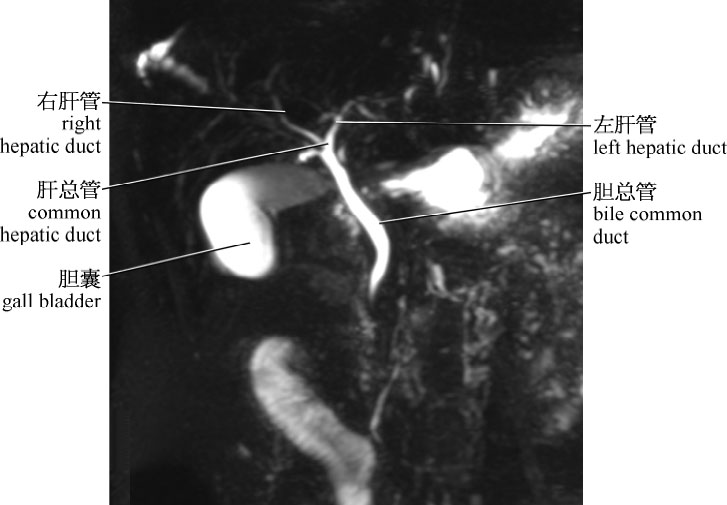
\includegraphics{./images/Image00164.jpg}
  \end{figure} 
 \FloatBarrier

\begin{figure}[!htbp]
 \centering
 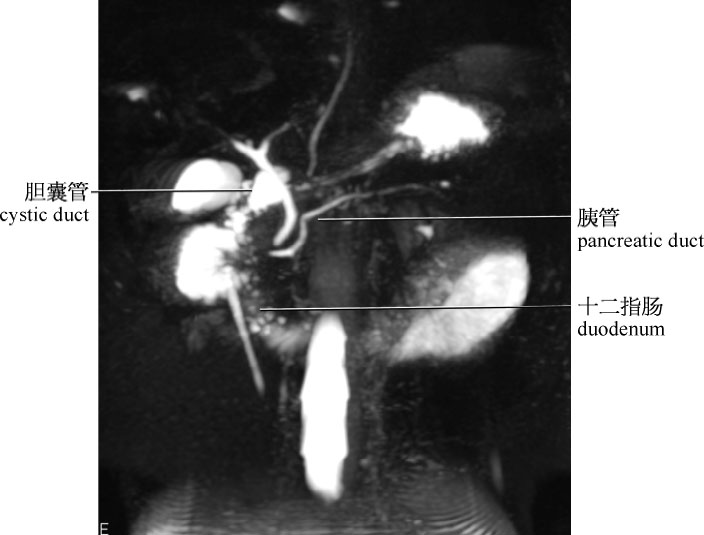
\includegraphics{./images/Image00165.jpg}
  \end{figure} 
 \FloatBarrier


\chapter{咯 血}

\section{12 咯血}

咯血是指喉及喉以下呼吸道或肺组织任何部位的出血,经口腔咳出者。咯血大多数为呼吸系统及(或)循环系统疾病所致,口腔、鼻腔或上消化道的出血有时易和咯血混淆。鼻腔出血多从前鼻孔流出,并常在鼻中隔前下方发现出血灶,较易诊断。有时鼻后部的出血量较多,特别是在睡眠时不自觉地坠入气道而于清晨咳出,较易误诊为咯血;如见血液从后鼻孔沿软腭或咽后壁下流,用鼻咽镜检查可以确诊。此外,还须检查有无鼻咽癌、喉癌、口腔溃疡、咽喉炎及牙龈出血的可能性。

呕血为上消化道出血,经口腔呕出,出血灶多位于食管、胃及十二指肠。咯血和呕血可根据病史、体征及其他检查方法进行鉴别,参见表\ref{tab4-1}。

\begin{table}[htbp]
\centering
\caption{咯血与呕血的鉴别}
\label{tab4-1}
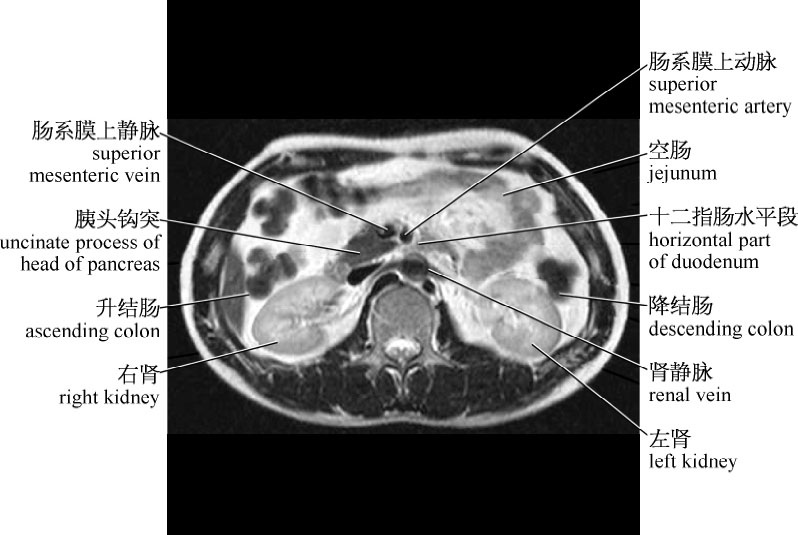
\includegraphics[width=5.89583in,height=2.59375in]{./images/Image00038.jpg}
\end{table}

区别咯血和呕血一般不难,但如患者出血急骤,量多或病史诉说不清时,有时鉴别并不容易;因此须详细询问有关病史,作细致的体格检查,及时作出诊断。

如已明确为咯血,须进一步探索其原因。引起咯血的原因很多(表\ref{tab4-2}),其中最常见的疾病是肺结核、支气管扩张、肺脓肿、支气管肺癌。此外支气管结石、肺寄生虫病、心血管疾病(特别是二尖瓣狭窄)、结缔组织病、钩端螺旋体病等也可引起咯血。

\begin{table}[htbp]
\centering
\caption{引起咯血的常见疾病分类}
\label{tab4-2}
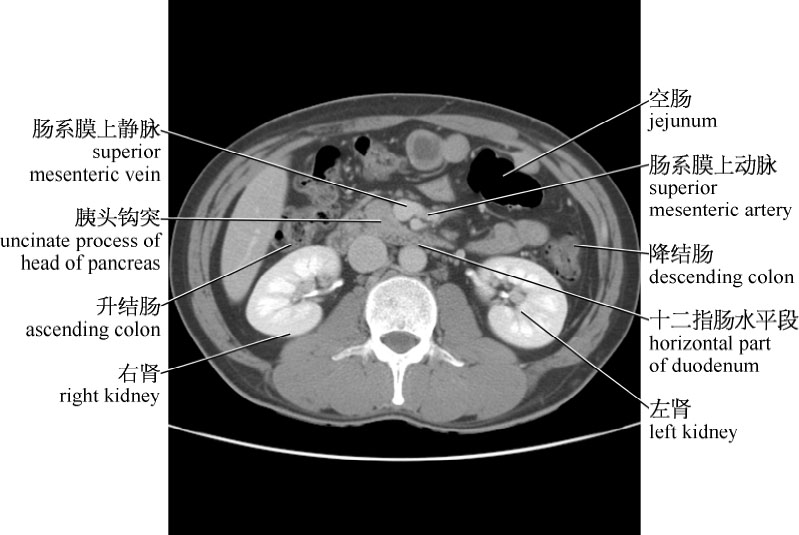
\includegraphics[width=5.89583in,height=4.80208in]{./images/Image00039.jpg}
\end{table}

如咯血量较大,应即采取急救措施,以尽早确定出血的部位。当X线检查的条件未具备时,可应用听诊法以确定。如咯血开始时一侧肺部呼吸音减弱或(及)出现湿啰音,而对侧肺野呼吸音良好,常提示出血即在该侧。气管和支气管疾病所致出血,全身症状一般不严重,胸部X线检查基本正常,或仅有肺纹理增粗;肺部病变所致出血,有比较明显的全身症状,胸部X线检查常发现病变阴影;必须指出,咯血可为全身疾病表现的一部分,临床医生必须对咯血患者做全身检查,以作出正确的诊断。

对于咯血患者,全面分析病史资料常可对咯血原因做出初步估计,同时还需要进一步做下列有关检查:

\subsection{1.病史}

须询问出血为初次或多次。如为多次,与以往有无不同。发生于幼年可见于先天性心脏病;儿童少年慢性咳嗽伴小量咯血和低色素性贫血,须注意特发性肺含铁血黄素沉着症;青壮年咯血多注意肺结核、支气管扩张等疾病;40岁以上有长期大量吸烟史(纸烟20支/
日×20年以上)者,要高度警惕支气管肺癌的可能性;年轻女性反复咯血也要考虑支气管结核和支气管腺瘤。在既往史上需注意幼年是否曾患麻疹、百日咳。在个人史中须注意结核病接触史、多年吸烟史、职业性粉尘接触史、生食螃蟹与蝲蛄史、月经史等。

细致观察咯血的量、颜色,有无带痰。肺结核、支气管扩张、肺脓肿、支气管结核、出血性疾病咯血颜色鲜红;肺炎球菌大叶性肺炎、肺卫氏并殖吸虫病和肺泡出血可见铁锈色血痰;烂桃样血痰为肺卫氏并殖吸虫病最典型的特征;肺阿米巴病可见脓血样痰呈棕褐色,带腥臭味;砖红色胶冻样血痰主要见于克雷伯杆菌肺炎;二尖瓣狭窄肺淤血咯血一般为暗红色;左心衰竭肺水肿时咳浆液性粉红色泡沫样血痰;并发肺梗塞时常咳黏稠暗红色血痰。大量咯血常由于空洞型肺结核、支气管扩张、慢性肺脓肿、动脉瘤破裂等所致;国内文献报告,无黄疸型钩端螺旋体病也有引起致命的大咯血。而痰中带血持续数周或数月应警惕支气管肺癌;慢性支气管炎咳嗽剧烈时可偶有血性痰。

详细询问伴随症状如发热、胸痛、咳嗽、痰量等。咯血伴有急性发热、胸痛常为肺部炎症或急性传染病,如肺出血性钩端螺旋体病、流行性出血热;咯血、发热同时伴咳嗽、咳大量脓痰多见于肺脓肿;长期低热、盗汗、消瘦的咯血应考虑肺结核;反复咳嗽、咳脓痰不伴有发热多见于支气管扩张。

\subsection{2.体格检查}

活动期肺结核和肺癌患者常有明显的体重减轻,而支气管扩张患者虽反复咯血而全身情况往往较好。有些慢性心、肺疾病可伴有杵状指(趾)。锁骨上淋巴结肿大在中老年患者要注意肺内肿瘤的转移。肺部闻及局限性哮鸣音提示支气管有狭窄、阻塞现象,常由肿瘤引起。肺部湿性啰音可能是肺部炎症的体征,也应考虑是否为血液存积在呼吸道所致。对咯血患者还应注意有无全身的出血表现。

\subsection{3.实验室检查}

痰检查有助于发现结核杆菌、真菌、癌细胞、肺吸虫卵等。出血时间、凝血时间、凝血酶原时间、血小板计数等检查,有助于出血性疾病的诊断。外周血红细胞计数与血红蛋白测定可推断出血的程度。外周血中嗜酸性粒细胞增多提示寄生虫病的可能性。

\subsection{4.X线检查}

对于咯血患者,除个别紧急情况不宜搬动外,均应做胸部X线检查。肺实质病变一般都能在X线胸片上显示阴影,从而及时作出诊断。如疑有空洞、肿块,或见肺门、纵隔淋巴结肿大,可加做胸部X线体层摄片或CT检查,CT还有助于发现细小的出血病灶。对疑有支气管扩张者,可做高分辨CT检查等协助诊断。对疑为支气管动脉性出血所致大咯血,必要时可行CT支气管动脉造影(CTA)或数字减影血管成像(DSA)检查,明确出血部位,后者尚可同时进行栓塞介入治疗。

\subsection{5.纤维支气管镜检查}

原因未明的咯血,尤其伴有支气管阻塞者,应考虑纤维支气管镜检查,可发现气管和支气管黏膜的非特异性溃疡、黏膜下层静脉曲张、结核病灶、肿瘤等病变,并可在直视下钳取标本作病理组织检查,吸取分泌物或灌洗液送细菌学和细胞学检查。

\subsection{6.其他检查}

先天性心脏病的诊断往往借助右心导管检查。放射性核素67镓对恶性肿瘤组织较健康组织有更大的亲和力,因而枸橼酸67镓肺部扫描可能有助于肺癌与其他肺部肿物的鉴别诊断。PET/CT对肺部肿瘤引起的咯血的诊断也有帮助。

咯血量的多少视病因和病变性质而不同,但与病变的严重程度并不完全一致,少则痰中带血,多则大口涌出,一次可达数百或上千毫升。临床上常根据患者咯血量的多少,将其分为少量咯血、中量咯血和大量咯血。但界定这三种情况的咯血量多少的标准尚无明确的规定,但一般认为24小时内咯血量少于100ml者为小量咯血;100~500ml/d者为中量咯血;>500ml或一次咯血量>100ml者为大量咯血。

临床上无异常肺部X线征象的咯血病例并不少见,诊断较为困难,其主要原因可能为:①气管或大支气管的非特异性溃疡,一般表现为小量咯血或血痰,支气管镜检查可以发现。②气管或支气管的静脉曲张,多见于右上叶支气管开口处或隆突部分,常引起大咯血,无痰,可经支气管镜检查而发现。③肺动脉瘤、支气管小动脉粥样硬化破裂,肺动静脉瘘破裂。④小块肺栓塞,常不易发现,一般有心脏病、下肢深静脉血栓形成、外伤史、长时间卧床或处于产褥期病史。⑤钩虫蚴、蛔虫蚴、血吸虫毛蚴、比翼线虫在肺内游移引起咯血。⑥早期支气管肿瘤,轻度支气管扩张、支气管结核,肺结核早期等。纤维支气管镜的广泛应用,结合胸部X线检查大大提高咯血病因的确诊率,国内一组917例经胸部X线与纤维支气管镜检查而确定的咯血病因如表\ref{tab4-3}所示:\footnote{*既有临床表现又有X线表现}

\begin{table}[htbp]
\centering
\caption{917例咯血的病因分析(X线诊断与纤支镜诊断比较)}
\label{tab4-3}
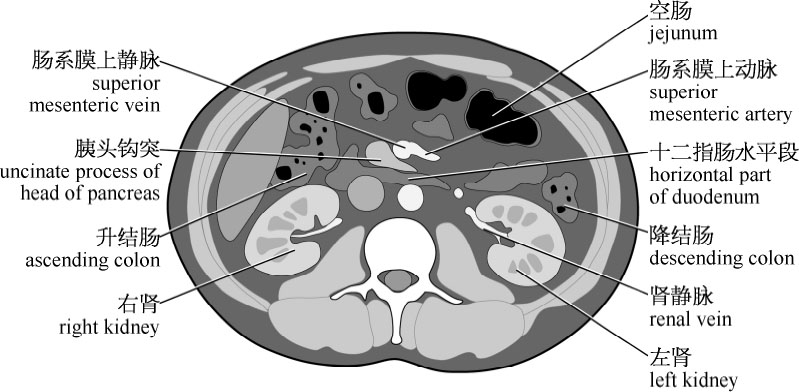
\includegraphics[width=5.91667in,height=3.58333in]{./images/Image00040.jpg}
\end{table}

由表\ref{tab4-3}所示,有部分咯血患者虽经X线和纤维支气管镜检查,仍未能发现阳性结果,且患者亦无引起咯血的全身性疾病,此类咯血可称为特发性咯血。但仍有可能在以后随诊中,在这类“特发性咯血”患者的一部分中,检出呼吸系统疾病。

国内曾有报告一组390例胸片无明显异常的咯血患者,作纤维支气管镜检查,结果发现肺癌16例(4.1\%)、支气管结核2例、支气管腺瘤1例,支气管囊性静脉曲张出血l例。作者认为咯血患者40岁以上,吸烟指数(吸烟年限×每天吸烟支数)>400,咯血时间长,且为痰血而非纯咯血者,尤须警惕肺癌的可能性。

X线胸片是咯血患者的常规检查,但可能无阳性发现。X线胸片正常的咯血患者应进一步作病因学诊断。有作者推荐应先作CT检查,以期发现潜在的肺部病灶,并有助于以后做纤维支气管镜检查时,有目标地进行刷检、活检取材,提高咯血的病因学诊断率。

\protect\hypertarget{text00057.html}{}{}

\subsection{12.1 气管和支气管疾病}

\subsubsection{一、急、慢性支气管炎}

急、慢性支气管炎患者有时也可咯血,一般为小量或痰中带血,不需治疗,可在数天内自行停止,但易于再发。如出血量大,需注意其他原因。本病的咯血与支气管炎症加剧有一定的关系,故咯血前常有病情加重的表现。慢性支气管炎患者发生持续的小量咯血时,须小心寻找其他原因,特别是支气管肺癌。

\subsubsection{二、非结核性支气管扩张}

非结核性支气管扩张可分为原发性与继发性。继发性者是由于支气管内或支气管外阻塞,引起支气管腔与支气管壁的感染,从而损害支气管壁的各层组织所引起。原发性支气管扩张则无明显的引起支气管阻塞的因素,但多数有肺炎病史,特别是麻疹、百日咳、流感等所继发的支气管肺炎史。

咯血是非结核性支气管扩张的常见症状,文献报告约90\%患者有不同程度的咯血,并作为提示诊断的线索。咯血可从童年即开始,常伴有杵状指(趾)。

此病的咯血有两种不同表现:

\paragraph{1.小量咯血}

在经常有慢性咳嗽、脓痰较多情况下,同时有小量咯血;有时在咯血前先有咳嗽较剧烈的一段感染加重阶段。因感染导致支气管内肉芽组织充血及损伤小血管而出现咯血。

\paragraph{2.大咯血}

由于支气管有炎症病变,血管弹性纤维被破坏,管壁厚薄不匀或形成假血管瘤,加上炎症影响,易破裂引起大咯血。咯血量每次达300~500ml以上,色鲜红,常骤然止血(因此类出血常来自支气管动脉系统,压力高,而动脉血管壁弹性好,收缩力强,故可较快止血)。

患者病程虽长,但全身情况尚好。咳嗽和咳痰也为常有的症状,咳嗽可轻微,也可相当剧烈;咳嗽和咳痰常与体位改变有关,如在晨起或卧床后咳嗽可加剧,咳痰增多。痰量可为大量,每天达数百毫升(湿性型)。痰液静置后可分为三层:上层为泡沫状黏液,中层为较清的浆液,下层为脓液及细胞碎屑沉渣。有些患者痰量甚少(干性型),如合并感染,痰量随之增多,并有发热、咯血等。

支气管扩张的好发部位是下肺,以左下叶较右下叶为多见,最多累及下叶基底段,病灶可延伸至肺边缘。病变部位出现呼吸音减弱和湿性啰音,位置相当固定,体征所在的范围常能提示病变范围的大小。

胸部X线平片检查不易确诊本病。国内一组84例非结核性支气管扩张中,只1/3病例在胸部X线平片上有少许的征象,大部分甚至没有任何改变。胸部X线平片检查对排除慢性肺脓肿及慢性纤维空洞型肺结核颇有帮助。如患者有支气管扩张的临床表现,X线胸片又显示一侧或双侧下肺纹理增粗、紊乱以及蜂窝状小透亮区,或见有液平面则支气管扩张的可能性最大,胸部CT检查可确定诊断,并对明确病变部位及决定治疗方案有重要意义。

全内脏转位、支气管扩张、鼻窦病变三联症,又称Kartagener综合征,国内有少数病例报告。此综合征有咳嗽、咳痰、咯血等症状。咯血可从童年开始,反复发作,量不多。

\subsubsection{三、结核性支气管扩张}

结核性支气管扩张的症状因肺内结核病灶的情况而定,如肺结核病灶不严重,则可无明显症状。有时或可闻及少许干、湿性啰音。X线胸片上显示病灶似已硬结,而患者仍有或多或少的咯血,应考虑结核性支气管扩张的可能性。国内一组64例患者中,发病大多在30岁以上,90\%有咯血(痰中带血或大量咯血)。病灶部位大都在两肺上叶,尤以右上叶的后段、左上叶的尖后段多见。

结核性支气管扩张与非结核性支气管扩张的鉴别见表\ref{tab4-4}。

\subsubsection{四、支气管结核}

支气管结核一般为继发性,原发性者罕见。患者大多有咯血,其他常见症状为阵发性剧烈咳嗽、喘鸣、阵发性呼吸困难等。有时轻度动作即可引起呼吸困难与发绀。如发生支气管阻塞,则引起突然的发热、痰量减少,而阻塞解除后痰量突然增加,体温也下降。

\begin{table}[htbp]
\centering
\caption{结核性与非结核性支气管扩张的鉴别要点}
\label{tab4-4}
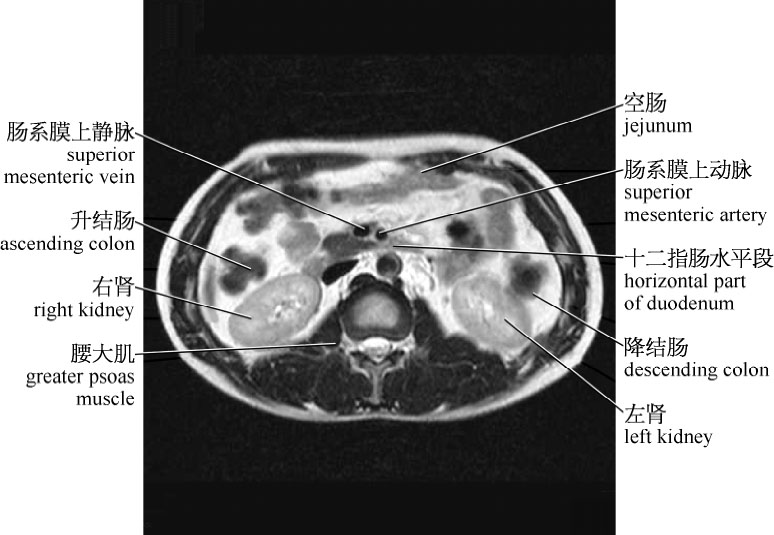
\includegraphics[width=5.94792in,height=1.65625in]{./images/Image00041.jpg}
\end{table}

支气管结核是发生于气管、支气管黏膜或黏膜下层的结核病变。据国内报告,肺结核合并支气管结核者占23.6\%~57.1\%。患者以青壮年为多,文献报告女性罹患多于男性,常发生于慢性纤维空洞型肺结核、慢性血行播散型肺结核、支气管淋巴结结核、浸润型肺结核及干酪样肺炎等基础之上。这些患者有下列情况提示有支气管结核的可能:①反复小量咯血或血痰而X线胸片未见明显病变者;②药物难以控制的刺激性咳嗽;③有喘鸣音;④有不同程度的呼吸困难而不能用肺实质病变解释者;⑤肺无明显病变而痰结核菌屡为阳性;⑥肺内有新播散病灶而不能用其他原因解释;⑦肺结核并发肺不张;⑧某些肺野空洞:在萎陷疗法后产生的张力性空洞;空洞时大时小;出现圆形、薄壁空洞;肺门附近的空洞等。

支气管结核的确诊须依靠纤维支气管镜检查。如临床症状典型,虽纤维支气管镜检查阴性,也不能除外此病的存在。

近年国内一组单纯气管、支气管结核病28例报道,误诊颇多,原因为:①胸片无异常发现;②胸片虽出现局限性肺气肿、肺纹理密集、肺纹理粗乱、叶间胸膜影移位等异常表现,但又非特异性而未加注意。作者建议对干咳、胸闷、喘息、咳黏液痰或咯血患者,经抗感染及对症治疗2周未见好转时.应及早作纤维支气管镜检查,镜下刷检涂片染色找抗酸杆菌,或钳取组织做病理检查。镜下所见仍疑似结核而实验室检查阴性时,2周后应再做纤维支气管镜检查。

目前将刷检标本或支气管肺泡灌洗液进行PCR检测结核分枝杆菌,可大大提高病原学诊断率。

结核感染T细胞斑点(T-SPOT.TB)试验是近年来的一项新诊断技术,通过检测外周血分泌γ-干扰素的T淋巴细胞数量来诊断结核感染,具有较高的特异性和敏感性,且不受卡介苗接种和环境分枝杆菌感染的影响,在肺结核的筛查和诊断中有较好的应用价值。

\subsubsection{五、支气管结石}

本病的特点为反复咯血,而肺部除有钙盐沉积之外,无其他原因可解释。患者或曾有咳出结石史。咯血通常为小量,但有些患者可有大咯血。X线检查发现有支气管结石阴影,以右中叶根部较为多见,结石远端可发现有阻塞性肺不张或肺部感染,CT检查可见支气管阻塞远端有钙化影。纤维支气管镜检查可帮助诊断。支气管结石常由肺结核病灶钙化引起。X线胸片上如炎症病变相应部位有钙化结节,在炎症消退后而咯血不断者,则支气管结石的可能性甚大。

据国内一组20例的报告中,以咯血为主要症状者占95\%,其中威胁生命的大咯血占40\%。误诊率60\%。并发症(占85\%)表现为肺不张、支气管扩张、阻塞性肺炎等。但手术治疗效果好。X线断层摄片、胸部CT和纤维支气管镜检查等综合检查对诊断有较大帮助。

\subsubsection{六、原发性支气管肺癌(肺癌)}

本病大多见于40岁以上男性,文献报告有咯血者占50\%~70\%,国内一组141例报告中,第一个月内出现咯血者有38.3\%。中央型肺癌较周围型肺癌易引起咯血。癌组织内小血管较多,患者又常有刺激性咳嗽,易引起癌组织损伤而致出血。其特点是痰中带血或小量咯血多见,而大量咯血少见,但晚期可有致命性大咯血。咳嗽是较常见的早期症状,无痰或有少量的白色黏液痰,可伴有胸痛。间断的或持续的小量咯血,对提示此病的诊断有重要意义。痰中可混有小颗粒状灰白色坏死组织,其中较易找到癌细胞。X线胸片、纤维支气管镜、胸部CT及活组织病理检查有助于诊断。

国内一组确诊肺癌患者1105例中,纤维支气管镜下直接见到肿瘤病灶(直接征象)者638例(57.7\%),只见肿瘤间接征象,即支气管黏膜改变者412例(37.3\%)。肺癌多见于段以上的支气管(中央型肺癌约占3/4),有些病例第一次活检及刷检均未能确诊,需做第二次,偶尔还要第3~4次检查。当发现有间接征象的可疑病例,应尽可能多部位活检多取标本,甚至看到癌体也应多点活检。

\subsubsection{七、支气管类癌}

支气管类癌罹患多为中年人,男女性别无差异,生长慢,具有恶性程度低和较少发生转移的特点。早期症状常为咯血,术后长期生存率较高。国内一组17例报告中,患者40岁以下者占64.7\%,中央型12例,周围型5例,2例有支气管旁淋巴结转移,主要临床表现为咳嗽、咳痰、咯血或痰中带血、发热和反复发作肺部炎症。临床上本病易误诊为肺癌、结核球或良性支气管肿瘤。X线检查与纤维支气管镜下活检对诊断帮助较大。

\subsubsection{八、良性支气管瘤}

良性支气管瘤少见,发病多在30~40岁之间。全身情况良好的中年患者如有反复的小量咯血或痰中带血,或类似哮喘发作,或屡次发作的呼吸道阻塞及感染症状,应考虑此病的可能。由于肿瘤生长缓慢,临床症状可延续多年。早期可无症状,或仅有气喘、干咳,有时甚至被误诊为支气管哮喘。肿瘤逐渐增大而堵塞支气管时,可发生相应肺叶的肺不张,并在肿瘤的远侧发生感染与支气管扩张。X线体层摄片、胸部CT,可了解较大的支气管内肿瘤的范围及部位,气道阻塞情况及继发性支气管扩张,对诊断有重要帮助。由于良性瘤多发生于较大的支气管内,纤维支气管镜检查的检出率可达85\%~90\%。

良性支气管瘤有腺瘤、平滑肌瘤、乳头状瘤等,此外较罕见的有纤维瘤、软骨瘤、脂肪瘤等。其中腺瘤比较多见,典型X线征象为肺门附近有圆形或类圆形阴影,密度均匀一致,边缘锐利,体层摄片或胸部CT检查更易于发现;由于多数腺瘤位于主支气管或肺叶支气管内,纤维支气管镜检查易作出诊断。

\protect\hypertarget{text00058.html}{}{}

\subsection{12.2 肺部疾病}

\subsubsection{一、肺结核}

咯血是肺结核患者常见的症状,且常为提示此病诊断的线索。咯血量多寡不一,少可仅为痰中带血,多则一次可达500ml以上,血色鲜红。咯血与结核病变的类型有一定关系,多见于浸润型肺结核、慢性纤维空洞型肺结核、干酪样肺炎,而少见于原发综合征(原发型肺结核)和急性血行播散型肺结核。咯血严重程度并不一定与病灶大小成正比,小的病灶可有较多的咯血,而病灶广泛的也可无咯血。出血量常和血管损害程度有关,血管壁渗透性增高所致的咯血,出血量少,但持续时间较长;小血管的破裂则多引起小量出血,这往往由于慢性活动性肺结核所致;大咯血多为肺动脉分支破损所致,其中以空洞内形成的动脉瘤破裂所致的大咯血多见,此类出血来势甚急,而由于洞壁纤维化不易收缩止血,或血凝块虽能填塞空洞压迫血管暂时止血,但又可因血块溶解而再次出血。

肺结核患者以青壮年占大多数,不少患者以咯血为初发症状而就诊。咯血之后常有发热,是由于病灶播散及病情发展所致。患者常同时出现疲乏、纳差、体重减轻、午后潮热、盗汗、脉快和心悸等全身中毒症状。

肺结核的诊断主要依靠症状、体征、X线胸片和痰结核菌检查。如在青壮年人一侧肺尖部经常听到湿性啰音,又有上述全身性中毒症状,则支持活动性肺结核的诊断。X线胸片是诊断肺结核的重要方法,可以发现早期轻微的结核病变,确定病灶的范围、部位、形态、密度、与周围组织的关系,判断病变的性质、有无活动性、有无空洞、空洞大小和洞壁特点等。因此,定期进行胸部X线检查能及早发现病灶,有助于早期治疗。

痰结核菌检查阳性可确诊为肺结核,且可肯定病灶为活动性。但痰结核菌阴性并不能否定肺结核的存在,对可疑病例需反复多次痰液涂片检查,如有需要,可采用浓集法、培养法、PCR法等,在咯血前后,因常有干酪性坏死物脱落,此时的痰菌阳性率较高。

长期被误诊为肺结核咯血的肺部疾病并非少见,文献报道有支气管扩张、支气管囊肿、肺癌、肺脓肿、肺吸虫病等。

年轻患者反复咯血,痰结核菌检查阴性,全身情况较好,而病灶又处于中、下肺野,用一般抗菌药物治疗能改善炎症表现者,则可认为是非结核性支气管扩张,胸部CT检查有助于确定诊断。支气管囊肿在胸部平片及透视下一般可确定诊断。非结核性支气管扩张或支气管囊肿合并普通细菌感染时,其症状的出现通常较早,可追溯到童年时期,特别是在患麻疹、百日咳之后常有咯血及呼吸道炎症症状,其与肺结核病的鉴别是前两者在长期的病患过程中,全身一般状况仍较好,无结核病的全身中毒症状,可伴有杵状指(趾),痰结核菌阴性。

肺癌被误诊为肺结核者颇为常见。在下列情况下,应考虑肺癌的可能:①年龄在40岁以上,尤其是长期重度吸烟的男性患者,新近出现反复的咯血或持续的痰中带血,或近肺门处有致密的异常阴影,或出现肺不张合并感染,而多次痰液检查未发现结核菌者,应首先考虑肺癌的可能;但痰中结核菌阳性也不能除外肺结核与肺癌并存。②肺癌组织内部发生坏死破溃,坏死组织排出后形成空洞,其X线征象可酷似结核性空洞。但癌性空洞常呈偏心性,其内侧壁凹凸不平,外缘多呈毛刺状、分叶状,常无病灶周围卫星灶,多次痰结核菌检查阴性,经规律的抗结核治疗无效,病灶逐渐增大,这些均可与肺结核鉴别。③肺癌和肺结核并存,肺癌可发生在陈旧性肺结核瘢痕的基础上,而肺癌又能促使结核病灶恶化。如在陈旧性或活动性结核病灶处出现新的、致密的圆形病灶,且经积极抗结核治疗一个月后,病灶仍逐渐增大,或出现肺不张、肺门阴影增大,癌性空洞等改变,应考虑并存肺癌的可能。

\subsubsection{二、肺 炎}

在急性肺炎时,肺实质处于高度充血状态,小血管通透性增加并可发生破裂而致咯血。由于小血管可发生血栓性脉管炎,致血管腔闭塞,通常不易引起大量咯血。

肺炎链球菌肺炎的患者,痰中混有血液者并不少见,有时血量可达20~30ml,病期第2、3天转为铁锈色痰。在整个病程中均呈血性痰的甚少。

肺炎杆菌性肺炎多为砖红色稠胶样痰;化脓性链球菌肺炎咳粉红色稀痰;葡萄球菌肺炎可为血性痰、脓性痰;绿脓杆菌肺炎咯血少见,典型者咳翠绿色脓痰。军团菌肺炎少量黏液痰中可带血丝,并有发热、咳嗽、肌痛、关节痛、腹泻、蛋白尿、转氨酶升高、直接荧光抗体阳性或间接荧光抗体1∶256。肺炎支原体肺炎约1/4病例有血性痰,但绝无铁锈色痰;流感病毒性肺炎常引起反复的小量咯血。

\subsubsection{三、肺脓肿}

肺脓肿多由于吸入感染或血源性感染所引起,约50\%患者伴有咯血,常伴有大量脓痰或脓血样痰。急性肺脓肿的早期可有大量的咯血而无脓痰,但此时有寒战、高热、胸痛、血白细胞和中性粒细胞增高,提示急性细菌性感染,1周后可出现大量脓性痰。慢性肺脓肿常有大量的脓痰或脓血痰,痰量每天可达300~500ml,带臭味,痰静置分层,多数患者伴有杵状指。慢性肺脓肿常被误诊为肺结核病,前者可根据急性发病史、X线胸片见大片浓密模糊浸润阴影,脓腔内出现圆形透亮区及气液平面,痰培养可有致病菌生长以及抗菌治疗有效,一般鉴别不难。慢性肺脓肿与肺癌的区别,可根据肺脓肿过去的急性发病史、空洞的特点及痰中癌细胞检查等加以鉴别,X线胸片、纤维支气管镜、胸部CT扫描有利于诊断。癌性空洞与肺脓肿空洞、结核性空洞的鉴别参见表\ref{tab4-5}。

\begin{table}[htbp]
\centering
\caption{癌性空洞与肺脓肿空洞、结核性空洞的鉴别}
\label{tab4-5}
\includegraphics[width=5.97917in,height=3.53125in]{./images/Image00042.jpg}
\end{table}

\subsubsection{四、肺部真菌感染}

肺部真菌感染是最常见的深部真菌病,主要由念珠菌、曲霉、毛霉、新型隐球菌等真菌感染所致。老年、幼儿及体弱者易患此病,多为痰中带血或小量咯血。常见症状有发热、乏力、盗汗、纳差、消瘦、咳嗽、胸痛;痰的特点是量少,不同种类的真菌感染时,其痰的性状不一。肺白念珠菌感染,为胶样黏稠痰,带乳块或血丝;肺曲霉病反复咯血或咳出大量泡沫痰(可带酒味);肺新型隐球菌病则咳小量黏液性痰或血丝痰。病原学检查可找到致病菌,胸部X线检查,肺组织病理检查有助于诊断。

\subsubsection{五、肺寄生虫病}

\paragraph{1.肺阿米巴病}

阿米巴性肺脓肿为肝阿米巴病并发症之一,也可来自肠道病灶。多数起病较慢,常有发热、乏力、消瘦、咳嗽、咳痰、右下胸痛并放射至右肩,少数呈急性发病,高热、胸痛、呼吸困难等,可有肝脏肿大体征。典型的痰液呈棕褐色而带腥臭味,有助于此病的诊断。如合并出血或混合感染,可呈血性或黏液脓血痰。痰液、胸腔积液或纤维支气管镜取病变坏死组织中查找到溶组织阿米巴滋养体可确诊。

\paragraph{2.肺吸虫病}

本病有严格的地区性,患者都曾有在疫区进食未煮熟的含有肺吸虫囊蚴的石蟹或蝲蛄史。病程中常反复的小量咯血,痰血混合多呈特殊的棕黄色或铁锈色,烂桃样血痰是肺吸虫病最典型特征。早期症状有畏寒、发热、脐周隐痛、腹泻,并有乏力、盗汗、纳差,2~3周后出现咳嗽、胸痛、咯血等,患者虽有长期的反复咯血,但全身情况尚好,胸部体征多不明显,可有皮下结节。常有血嗜酸性粒细胞增多,痰中发现肺吸虫卵即能确诊,阳性率90\%以上。粪便虫卵检查、肺组织病理检查、免疫学检查、X线检查等有助于诊断。

胸部X线检查有较特别的征象,病灶多位于中、下肺野及内侧带,因病变的不同时期而有下列的表现:①早期呈边缘模糊的弥漫阴影,大小约为1~2cm;②中间期为边缘清楚、多房或单房的、实质或囊状的大小不等的阴影,多房性囊状阴影是本病的X线特征;③晚期为纤维增殖性变及硬结钙化阴影。此外,可有肺门增大、肺纹理增粗紊乱、胸腔积液或胸膜增厚等征象。对一些疑难的、不典型的病例,流行病学调查和免疫学检查,在诊断上有重要意义。

如患者有上述的流行病学史和胸痛、咳铁锈色痰等症状,血嗜酸性粒细胞增多,痰中虽未发现肺吸虫卵,而肺吸虫抗原皮内试验阳性,并已除外血吸虫病、华支睾吸虫等感染时,则大致可作出肺吸虫病的临床诊断,并应进行特效药物(如吡喹酮)的诊断性治疗;如疗效显著,可进一步确立诊断。肺吸虫病主要须与肺结核相鉴别(表\ref{tab4-6})。

\begin{table}[htbp]
\centering
\caption{肺吸虫病与肺结核鉴别}
\label{tab4-6}
\includegraphics[width=5.94792in,height=4.91667in]{./images/Image00043.jpg}
\end{table}

在四川及福建发现的肺吸虫病,临床表现较特别,其症状轻,咯血量较小,痰中虫卵检出率较低,有游走性皮下结节者甚多(多分布于胸壁及上腹壁),血中嗜酸性粒细胞显著增多。

国内报道肺吸虫病误诊率较高。主要原因是由于肺吸虫病临床表现及X线胸片大多无特异性,且典型的游走性皮下结节,肺空泡、结节和隧道线条等X线表现又少见。一组报道34例肺吸虫病在入院前全部误诊为肺结核。

由于肺吸虫病免疫学诊断的敏感性和特异性高,且简便易行,在流行区内患者有生食石蟹或蝲蛄史,而反复出现咳嗽、咯血或痰中带血、发热等症状,应即作肺吸虫抗原皮内试验,上述一组误诊为肺结核的34例患者,肺吸虫抗原皮内试验全部为1∶2000以上阳性。应用混合单抗双抗体夹心ELISA法诊断疑难肺吸虫病,效果更佳。

\paragraph{3.肺包虫病}

肺包虫病是棘球绦虫的幼虫(棘球蚴)寄生于人体肺内所引起,主要流行于畜牧区,以青壮年农民和牧民为主,早期可无症状。当包囊肿大破裂时可出现咯血或痰中带血,并可咳出类似粉皮样的角皮膜;合并感染时则出现咳嗽、咳痰、胸部不适,或胸痛及劳力后气促等症状。可有肝脏或其他部位囊肿征象。囊肿破裂,囊液亦可阻塞气管而引起窒息。X线胸片或CT扫描有助于诊断,可显示包虫圆形或卵圆形,略呈分叶状阴影,边缘清晰,密度均匀,壁可钙化,阴影随呼吸而变形;包虫囊壁破裂,空气进入,则顶部呈现半月形透亮带。包虫抗原皮内试验及补体结合试验对本病有重要的诊断意义,阳性率可达90\%以上。此外,痰检查、B超检查、放射性核素扫描等对诊断也有帮助。

\subsubsection{六、恶性肿瘤的肺转移}

恶性肿瘤转移至肺部时,可引起咯血。较常发生肺部转移的恶性肿瘤有鼻咽癌、乳腺癌、食管癌、胃癌、肝癌、结肠直肠癌、前列腺癌、睾丸畸胎瘤、精原细胞瘤、绒毛膜上皮细胞癌、恶性葡萄胎及类癌等。以绒毛膜上皮细胞癌、睾丸畸胎瘤和恶性葡萄胎的肺转移的咯血发生率最高。对成年女性原因未明的咯血,患者阴道曾排出水泡样胎块,或兼有流产后持续的不规则阴道出血,应考虑恶性葡萄胎或绒毛膜上皮细胞癌的可能性,尿妊娠诊断试验有助于此病的诊断。

转移性肺恶性肿瘤常为多发,但也可为单发,后者较少见。X线胸片显示多发性肺转移肿瘤的形态多为圆形、卵圆形或粟粒状阴影,大小相仿,边缘不整,发展较快。转移性肺恶性肿瘤原发病灶的诊断有时不易,须设法寻找。

\subsubsection{七、肺梅毒}

本病极为少见,国内仅有二例感染报告,均有咯血。病程进展缓慢,往往有咳嗽、咯血、胸痛等症状,虽然X线胸片显示下肺野呈大片状实质模糊阴影,但全身情况良好。诊断须依据梅毒感染史、梅毒血清反应阳性与驱梅治疗的疗效。肺梅毒须与其他肺部疾病相鉴别,特别是肺结核病。

\subsubsection{八、肺囊肿}

肺囊肿可区分为先天性与后天性两类,以前者较为多见,后者是由肺部感染性疾病或寄生虫所引起。多发性先天性肺囊肿常伴有支气管扩张,多在儿童期出现症状,其临床表现与支气管扩张相似,患者往往因突然小量咯血或痰中带血而就诊,由于病变多位于中、上肺,引流较好,较少出现发热。X线胸片检查呈圆形透亮影,其壁菲薄而整齐;多发者大小不一,可分布于任何肺野,但以中、上肺野较多见。

多发性先天性肺囊肿需与支气管扩张鉴别。肺囊肿继发感染时可出现大片状模糊阴影,类似浸润性肺结核,但经抗生素治疗后感染较快消退,而有别于肺结核。肺囊肿合并感染时,其临床症状和X线胸片的改变与肺脓肿相似,需加以鉴别。

国内曾报告一组82例的成年患者中,52例(63.4\%)有咯血,多数在200ml以下,认为如有下列情况应考虑本病:①肺部阴影长期存在;②阴影在同一部位反复出现;③无播散灶;④阴影新旧程度一致;⑤肺门及纵隔淋巴结不大。患者虽反复咯血而无结核中毒症状。胸部CT检查有助于对本病的诊断。

近年肺囊肿有一组38例报告,发病常在青少年期,5例初发年龄在10岁以下。全部患者(38例)在院外均被误诊为肺结核。初发症状以咯血或痰中带血多见(21/38),咳嗽、咳痰、发热次之。6例无症状患者经体检而发现本病。21例有长期反复出现咯血或痰中带血史,最长者达20年。

肺囊肿的胸部X线表现常缺乏特征性。作者认为以下几点有利于肺囊肿的早期诊断:①发病年龄在30岁以下,特别是男性,有反复咯血或痰中带血、咳嗽、发热史。②动态观察X线胸片阴影的形态变化不大,无肿瘤的淋巴结、淋巴道远处转移的改变。③结核菌素试验阴性或经积极的抗结核治疗无效。④胸部X线显示其病变虽无固定部位但与支气管走向有关;虽经反复感染但病变部位固定不变;在非囊肿部位不出现新的病灶。⑤有条件时应作高分辨胸部CT检查加以鉴别。⑥经上述不能确诊时应考虑肺活检或外科手术探查。

\subsubsection{九、尘 肺}

包括硅沉着病和其他尘肺,是由于长期吸入某种粉尘所致的以肺实质弥漫性纤维病变为主的疾病。主要发生于从事粉尘作业的工人,可有慢性、顽固性咳嗽,咳泡沫状痰、咯血或痰中带血,气短和胸痛。早期症状不明显,常为干咳或带黏稠痰,晚期咳嗽加重,痰多,如合并肺结核或支气管扩张,可反复大咯血。晚期病情重,有发绀、杵状指、肺气肿、肺源性心脏病等表现。胸片可见中、下肺野呈网状、条索状或结节状阴影改变,肺门淋巴结肿大。其诊断主要依据为职业病史、临床表现、胸部X线征象及肺功能检查。

硅沉着病合并肺结核比无硅沉着病的发病率高4~5倍,其特点是肺结核的发生率和严重程度与硅沉着病的发展程度成正比,硅沉着病愈严重,其并发肺结核的可能性愈大,肺结核病的病变发展也愈迅速,病情愈严重。石棉肺合并肺结核比较少见,但合并肺癌者却较多。

\protect\hypertarget{text00059.html}{}{}

\subsection{12.3 肺血管及其他循环系统疾病}

\subsubsection{一、肺血栓栓塞症}

肺血栓栓塞症是肺栓塞的最常见类型,占肺栓塞中的绝大多数,多继发于右心或体循环深静脉系统的血栓形成,偶尔也见于肺动脉炎、感染性心内膜炎等病例中,是以各种栓子阻塞肺动脉系统为其发病原因的一组疾病或临床综合征。主要症状为呼吸困难及气促、胸痛、小量咯血(大咯血少见)、咳嗽、心悸、发热等。心瓣膜病(特别是合并心房颤动)患者发生咯血、未能解释的短期发热时,须考虑肺血栓栓塞症的可能。X线胸片可显示区域性肺纹理变细、稀疏或消失,肺野透亮度增加;也可显示肺组织的继发改变,如肺野局部的片状阴影,尖端指向肺门的楔形阴影,肺不张或膨胀不全,有肺不张侧可见横膈抬高。X线胸片对鉴别其他胸部疾病有重要帮助。螺旋CT、放射性核素肺通气/血流灌注扫描、磁共振显像(MRI)及肺动脉造影都是肺血栓栓塞症的重要确诊方法。

\subsubsection{二、肺动脉高压}

肺动脉高压可由许多心、肺和肺血管疾病引起,根据发病的原因是否明确,曾被习惯性分为“原发性”和“继发性”肺动脉高压。2008年世界卫生组织第4届肺动脉高压会议重新修订了肺动脉高压分类,目前按照病因或发病机制、病理与病理生理学特点分为五个大类:①动脉性肺动脉高压;②左心疾病所致肺动脉高压;③肺部疾病及(或)低氧所致肺动脉高压;④慢性血栓栓塞性肺动脉高压;⑤未明多因素机制所致肺动脉高压。继发性肺动脉高压较原发性肺动脉高压常见,早期临床表现以基础疾病如慢性支气管炎、COPD等的临床表现为主,晚期以右心功能不全的表现为主。原发性肺动脉高压是一少见病,被世界卫生组织改称为“特发性肺动脉高压”,是一种不明原因的肺动脉高压。早期通常无症状,仅在剧烈活动时感到不适;随着肺动脉压力的增高,可逐渐出现呼吸困难、胸痛、头晕或晕厥、咯血。咯血量通常较少,有时也可因大咯血而死亡。其他症状还包括疲乏、无力,雷诺现象,声嘶(Ortner综合征)等。胸部X线检查、超声心动图和多普勒超声检查、放射性核素肺通气/灌注扫描、右心导管术、肺活检都对诊断有重要的作用。

\subsubsection{三、肺动静脉瘘}

肺动静脉瘘是先天性肺血管的血管瘤样畸形,也可为获得性,临床上少见。可有咳嗽、间歇小量咯血、发绀、杵状指(趾)及红细胞增多症。体格检查可发现在相应胸壁部位触及震颤,闻及来回性血管杂音。X线胸片和胸部CT在诊断上起重要作用,可见边缘整齐、密度均匀的圆形或卵圆形阴影,多位于中下肺野,且与肺门之间有条索状阴影,病变无钙化,无空洞形成。肺动静脉瘘发病常与遗传性出血性毛细血管扩张症有关,可误诊为肺结核球或支气管肺癌,肺动脉造影可协助明确诊断。

\subsubsection{四、单侧肺动脉发育不全}

本病少见,患者大多有不同程度的咳嗽、咳痰、痰中带血、胸痛、气促等表现,体格检查可发现患侧胸廓扩张稍受限、语颤及呼吸音减弱、多可听到干、湿性啰音,可被误诊为肺气肿、气胸、支气管扩张等。诊断主要依靠胸部X线检查,尤其是胸部CT的肺动脉造影对诊断极有帮助。

\subsubsection{五、肺淤血}

常见于风湿性心脏病二尖瓣狭窄,且多发生在较严重的瓣口狭窄的慢性充血期,也可见于急性左心衰、复张后肺水肿、高原性肺水肿等,多表现为痰带血丝、小量咯血或咳出粉红色泡沫样痰。结合心脏病史、胸腔快速抽液(气)及快速登山等病史,心尖部舒张期隆隆样杂音,超声心动图和多普勒超声检查等可作出诊断。二尖瓣关闭不全较少引起咯血。

\subsubsection{六、高血压}

在恶性或急进型高血压,由于血压持续增高时,可引起肺毛细血管破裂而出现咯血。也可由于并发急性肺水肿而咳粉红色泡沫样痰。

\subsubsection{七、先天性心脏病}

某些有血液分流的先天性心血管病如房间隔缺损、室间隔缺损、艾森曼格综合征等,均可伴有显著的肺动脉高压,由此可引起咯血。

\protect\hypertarget{text00060.html}{}{}

\subsection{12.4 全身性疾病及其他原因}

\subsubsection{一、急性传染病}

1.肺出血型钩端螺旋体病
肺出血型钩端螺旋体病也称钩端螺旋体性出血性肺炎,是钩端螺旋体病的严重类型,如不注意常易误诊。钩端螺旋体病以夏秋季多发,以青壮年为主,从事牧、渔业劳动者发病率高,大多起病急骤,症状主要有畏寒或寒战、高热、头痛、全身肌肉酸痛、衰弱无力、眼结膜充血、腓肠肌疼痛、淋巴结肿大,多在毒血症过程中出现心悸、烦躁、呼吸和心律逐渐增快。初为痰中带血,以后咯血量增多。严重的肺弥漫性出血型者,可引起致命的大咯血,其特点是发生突然、发展迅猛,临终时多数患者出现从口鼻涌出大量血液,立即窒息而死。X线胸片和胸部CT显示双侧肺野斑片状模糊阴影,以中、下肺野尤其显著。需与其他原因的肺炎、肺结核鉴别。病原学和血清学检查有助于明确诊断。

2.流行性出血热
由汉坦病毒引起,经呼吸道、消化道、母婴、虫媒及动物源传播,流行季节以3~5月份或5~7月份以及11月份至次年1月份间为高峰,青壮年多见,主要损害全身小动脉和毛细血管。患者起病急,典型病例具有发热、出血与肾损害三大主要特征以及发热期、低血压休克期、少尿期、多尿期和恢复期五期经过。其主要临床表现为发热、头痛、腰痛、眼眶痛、口渴、呕吐、酒醉貌、球结膜充血水肿,皮肤和黏膜广泛出血、鼻出血、咯血、呕血、便血、血尿,软腭及腋下有出血点,肾区有叩击痛。早期外周血白细胞正常或偏低,有尿蛋白,尿红、白细胞及管型改变;肾功能损害,约有半数出现肝功能损害。特异性血清学试验有助于确诊。

\subsubsection{二、血液病}

某些血液病如血小板减少性紫癜、白血病、再生障碍性贫血、血友病等均可出现咯血,与原发病有关。除咯血外,尚伴有其他部位的出血倾向。血常规、骨髓细胞学检查、血小板功能与凝血因子检查可确诊。

\subsubsection{三、白塞病(Behcet disease)}

本病由病毒感染、遗传因素、免疫功能及体内微量元素异常等因素引起。初发年龄主要是16~40岁的青壮年,以女性多见。基本病变是血管炎,可累及毛细血管和细小动静脉,可因肺部血管受累而反复咯血,多为小量咯血,也有因肺脉管炎而引起多发性肺栓塞。主要的临床表现为反复发作的口腔黏膜、舌尖及其边缘、齿龈、上下唇内侧等处的痛性小溃疡;外生殖器损害与口腔基本相似;眼部损害主要为结膜炎、角膜炎、虹膜炎、视网膜炎,其他表现有皮肤损害、消化道损害、关节损害及神经系统损害等。活动期多有血沉、黏蛋白、唾液酸、α2球蛋白增高,部分患者血浆铜蓝蛋白及冷球蛋白阳性。本病并发肺脉管炎引起咯血时的胸部X线表现,可类似肺炎支原体肺炎、肺部转移癌,或出现大片密度增高的圆形阴影。病理学检查及有关脏器病变的相应检查有助于诊断。针刺反应阳性是一特征性表现,若能同时检查HLA-B5,对本病的诊断更有帮助。

\subsubsection{四、结缔组织病}

该类疾病如系统性红斑狼疮、结节性多动脉炎、重叠综合征等,其发病与遗传、某些药物、物理因素、病毒感染、内分泌因素、免疫异常等有关,多见于20~40岁的女性。可有小量咯血,如伴有肺动脉受侵害,可发生大咯血。若患者有多个器官系统功能的损害,胸部X线检查见肺部有阴影,而抗菌药物治疗效果不佳时,应考虑结缔组织病伴有肺部损害的可能性。诊断结缔组织病所致的咯血时,须认真除外肺结核、支气管扩张、肺肿瘤等疾病。实验室检查和肺组织病理检查有助于诊断。

\subsubsection{五、肺出血-肾炎综合征}

国外文献曾有多例重度肺出血合并肾小球性肾炎报告,并命名为Goodpasture综合征,病因未明,也有将此病归入结缔组织病,临床上少见。此病多见于20~40岁男性,病程数月至数年,预后不良。临床经过可分为两个阶段:①肺部病变阶段,87\%~96\%以上的病例的首发症状表现为间歇的咯血,轻者为血痰,重者出现大咯血,反复出血可致贫血;病变广泛者可有呼吸困难、发绀与胸痛,X线胸片上显示短暂的弥漫性细小或大片状阴影,但X线检查也可呈阴性。②肾脏病变阶段:多数患者在咯血后数周或数月出现肾炎症状,肾脏病变表现为肾小球性肾炎,起病隐袭,当肺部病变显著时,尿检查发现蛋白尿、镜下血尿与管型尿,早期肾功能正常,当肾脏病变为进行性,尿毒症症状迅速出现,并掩盖肺部症状。X线、痰涂片、尿常规、血液检查、免疫学检查、肺功能检查都有助于诊断。肾组织活检免疫荧光检查,发现抗肾小球基底膜抗体则可明确诊断。通常由于尿毒症导致死亡。

除肺、肾两脏器之外,其他脏器很少受累。高血压少见。

\subsubsection{六、肉芽肿性多血管炎(韦格纳肉芽肿)}

是一种原因未明的综合征,被认为是机体对未知抗原的异常超敏反应所致。以30~50岁男性多见,具有上下呼吸道坏死性肉芽肿性血管炎,肾小球肾炎和小血管炎的临床表现。常有小量咯血,严重者可发生大量肺泡性出血,患者可伴有发热、乏力、纳差、关节痛、肌痛;上呼吸道症状有鼻分泌物增多、口咽部溃疡、声嘶;肺部症状有咳嗽、胸痛、呼吸困难;肾损害表现有不同程度的蛋白尿、镜下血尿或红细胞管型;其他表现可有皮肤黏膜损害、血疱、结节、红斑、结膜角膜炎、多发性神经炎、心肌炎、耳部损害。胸部X线检查表现为肺单侧或双侧多发或孤立结节影,大小不等,边界清楚,多有空洞形成,空洞壁薄而形态不规则,罕有液平存在。口咽、肺、肾组织活检及实验室检查有助于诊断,典型病例胞浆型抗中性粒细胞胞浆抗体(c-ANCA)阳性。

\subsubsection{七、弯刀综合征}

弯刀综合征为一种罕见的先天性血管畸形,其特征为右肺静脉开口于下腔静脉,X线胸片显示血管形态类似古代土耳其武土佩带的弯刀。患者常有反复咳嗽、咯血、右肺感染,易被误诊为“支气管扩张”。胸部X线检查为:①右肺发育不全;②X线检查沿右心缘的肺静脉呈弯刀样阴影;③心脏向右移位,状似右位心,据此可作出诊断。

\subsubsection{八、替代性月经}

成年女性发生与月经期相应的周期性咯血,须考虑为“替代性月经”。国内文献报告一例每次咯血都在月经周期前2~3天开始,待月经过后即能自行停止。此种异常现象罕见,原因未明,有人认为体内雌激素的周期性浓度增高,引起肺毛细血管充血、出血所致。部分患者在咯血周期前1周,应用黄体酮治疗可预防出血。此外,气管或支气管子宫内膜异位也可引起此现象,但罕见。

对此类与月经周期有明显关系的周期性咯血,须经细致检查与长期观察,而不能发现咯血

的其他原因时,方可下“替代性月经”的诊断。

(周燕斌 谢灿茂)

\protect\hypertarget{text00061.html}{}{}

\section{参考文献}

1.孙书明,等.138例咯血患者的胸部X线检查与纤维支气管镜检查对照分析.中华结核和呼吸杂志,1995,18(4):226

2.来孺牛.纤维支气管镜、螺旋CT对咯血的诊断价值.现代中西医结合杂志,2004,6:352

3.姜静波,等.CTA与DSA对支气管动脉性咯血临床应用价值的比较.医学临床研究,2012,29(7):1334-1337

4.宋美君,等.多层螺旋CT支气管动脉造影与数字减影下经股动脉支气管动脉造影在咯血诊治中的对比.中国呼吸与危重监护杂志,2012,11(4):378-381

5.胡华成,等.X线胸片正常咯血患者病因的进一步诊断.中华结核和呼吸杂志,1994,17(6):377

6.陈志烈,等.胸片无明显异常的支气管扩张症青年患者咯血的诊断与鉴别.宁夏医学院学报,2001,23
(1):28

7.林金学,等.单纯气管、支气管结核病28例临床分析.中华结核和呼吸杂志,1997,20(6):368

8.杨远,等.纤维支气管镜检讨胸片正常的支气管内膜结核.中华结核和呼吸杂志,1995,18(1):12

9.陈文彬,等.酷似肺癌的支气管结核六例.中华结核和呼吸杂志,1995,18(4):246

10.张立华,等.T-SPOT与结核菌素试验对结核病患者的临床诊断价值.中华临床医师杂志(电子版),2012,6(14):4107-4108

11.高明乐,季卫星.支气管壁内结石致大出血介入治疗1例.临床荟萃,1998,13(22):1040

12.林耀广,等.肺癌在支气管镜下的特征.中华内科杂志,1998,37(4):235

13.张逊,等.支气管类癌外科治疗11例报告.中华结核和呼吸杂志,1995,18(1):40

14.张兵,雷发国.34例肺吸虫病误诊临床分析.中华传染病杂志,1998,16(1):54

15.刘云霞,等.混合单抗双抗体夹心ELISA法诊断疑难肺吸虫病二例.中华内科杂志,1997,36(6)420

16.王维山,等.38例支气管囊肿临床及X线形态分析.中华结核和呼吸杂志,1994,17(5):314

17.易善国,等.弯刀综合征一例.中华内科杂志,1992,31(3):176

18.陈庆荣,等.Goodpasture综合征(附7例)报告及文献复习.中华肾脏病杂志,1991,7(2):93

19.毕经瑞.支气管子宫内膜异位症引起咯血1例报告.吉林医学,1998,19(6):333

\protect\hypertarget{text00062.html}{}{}


\chapter{急性呼吸衰竭与急性呼吸窘迫综合征}

\section{前沿学术综述}

\subsubsection{历史发展}

急性呼吸窘迫综合征(ARDS)是急性呼吸衰竭最常见的类型。1967年Ashbaugh观察到12例重症患者(7例严重创伤、1例急性胰腺炎、1例病毒性肺炎、1例吉兰-巴雷综合征合并肺炎、2例药物中毒合并误吸),在原发病治疗过程中,均出现类似急性呼吸衰竭表现:呼吸频速、低氧血症、肺顺应性明显降低、肺泡表面张力明显升高。X线胸片早期为双肺斑片状浸润阴影,随病情进展,浸润阴影进一步扩大。最后9例患者死亡,其中7例尸检,发现肺重量明显增加,而且变硬,肺切面类似肝脏。光镜检查显示肺毛细血管充血、扩张,广泛肺泡萎陷,并有大量中性粒细胞浸润,肺泡内有透明膜形成。部分尸检标本有明显的间质纤维化。患者的低氧血症不能被吸氧等传统治疗手段纠正,但呼气末正压(PEEP)能够部分纠正低氧血症。鉴于上述患者有类似临床表现、病理结果和治疗反应,Ashbaugh将其归结为“成人呼吸窘迫综合征(亦为ARDS)”。4年后,“成人呼吸窘迫综合征”被正式推广采用。根据病因和病理特点不同,ARDS还被称为休克肺、灌注肺、湿肺、白肺、成人透明膜病变等。

近年来,许多学者认识到“成人呼吸窘迫综合征”这一名称并不合适。并非仅发生在成人,儿童亦可发生。ARDS的特点在于急性起病。因此,为澄清并统一概念,1992年欧美危重病及呼吸疾病专家召开了ARDS联席会议
\protect\hyperlink{text00011.htmlux5cux23ch1-10}{\textsuperscript{{[}1{]}}}
,将ARDS中的“A”由成人(adult)改为急性(acute),称为“急性呼吸窘迫综合征”。以往认为,ARDS是肺部遭受直接损伤的结果,目前认为各种原因导致机体失控的炎症反应才是ARDS的根本原因,急性肺损伤与ARDS是连续的病理生理过程,ARDS并不是孤立的疾病,而是多脏器功能障碍综合征(MODS)在肺部的表现。

\subsubsection{流行病学}

流行病学调查显示,ARDS是临床常见危重症。根据1994年欧美联席会议提出的ALI/ARDS诊断标准
\protect\hyperlink{text00011.htmlux5cux23ch1-10}{\textsuperscript{{[}1{]}}}
,ALI发病率为每年18/10万,ARDS为每年(13~23)/10万。2005年的研究显示,ALI/ARDS发病率分别在每年79/10万和59/10万
\protect\hyperlink{text00011.htmlux5cux23ch2-10}{\textsuperscript{{[}2{]}}}
,提示其发病率明显增高,甚至可与胸部肿瘤、AIDS、哮喘或心肌梗死等相提并论
\protect\hyperlink{text00011.htmlux5cux23ch3-10}{\textsuperscript{{[}3{]}}}
,显著增加了社会和经济负担。

虽然不同研究对ARDS病死率的报道差异较大,但总体来说,目前ARDS的病死率仍较高。自1994年达成ARDS诊断共识以来,ARDS总体病死率并无明显降低。对1994~2006年国际正式发表的ARDS临床研究进行荟萃分析,18900例ARDS患者的病死率为44.3%,与1967~1994年病死率(30%~50%)相比并无明显降低
\protect\hyperlink{text00011.htmlux5cux23ch4-10}{\textsuperscript{{[}4{]}}}
。中国上海市15家成人重症医学科2001年3月至2002年3月ARDS患者的病死率也高达68.5%
\protect\hyperlink{text00011.htmlux5cux23ch5-10}{\textsuperscript{{[}5{]}}}
。不同研究中,ARDS的病因构成、疾病状态和治疗条件的不同可能是导致其病死率不同的主要原因。

\subsubsection{治疗进展}

在治疗过程中不应把ARDS孤立对待,而应该将其视为多脏器功能障碍综合征的一部分。在呼吸支持治疗的同时,应特别重视对于原发病的治疗和其他脏器功能支持治疗。近年来,体外膜氧合技术的应用为进一步降低重症ARDS患者的病死率带来了新的希望。此外,针对ARDS肺损伤本质的干细胞治疗也受到越来越多的关注,可能为ALI/ARDS的治疗开辟新的途径,但目前仍处于动物实验阶段。

(1)原发病治疗 及时去除或控制致病因素是ARDS病因治疗的重要环节,根据ARDS的病因不同,主要包括充分引流感染灶、有效地清创和合理使用抗生素等。机体过度的炎症反应是导致ARDS的根本原因,调控机体的炎症反应是ARDS病因治疗的关键。虽然在动物实验中,应用单克隆抗体或拮抗剂可明显减轻肺损伤,但多数临床试验却获得阴性结果。目前,在调控机体炎症反应方面尚未取得突破性进展,但调控炎症反应仍然是降低ARDS患者病死率的希望。呼吸支持治疗从本质上来说,不可能从根本上改善ARDS患者的预后,因此,对调控机体炎症反应进行更深入研究非常必要。

(2)呼吸支持治疗 机械通气是ARDS呼吸支持治疗的主要方法,也是目前发展较为迅速的领域。近年来,基于对ARDS的病理生理和呼吸机相关性肺炎的新认识,一些新的通气策略逐步应用于ARDS的临床治疗,体外膜氧合技术的应用使保证气体交换的同时减缓肺损伤成为可能,为患者呼吸功能的修复赢得了时间。

肺保护性通气策略:由于ARDS患者大量肺泡塌陷,肺容积明显减少,常规或大潮气量通气易导致肺泡过度膨胀加重肺损伤,因此,为避免或减轻机械通气所致的肺损伤,主张对ARDS患者进行机械通气时应采用小潮气量(一般4~7ml/kg)通气,即肺保护性通气。近年来,人们逐步意识到小潮气量并非是避免肺损伤的关键因素,而气道平台压力能够客观反映肺泡内压,气道平台压力过度升高可导致呼吸机相关肺损伤。目前认为,ARDS肺保护性通气策略的关键是将气道平台压限制在30cm
H\textsubscript{2} O(1cm H\textsubscript{2} O=0.098kPa)以下。

肺开放策略:限制气道平台压往往不利于已塌陷的肺泡复张,采用肺保护性通气策略的同时,实施肺开放策略是非常必要,其核心是采用各种方法促进塌陷的肺泡复张,即“开放肺”,并应用最佳呼气末正压保持肺泡处于开放状态,即“维持肺开放”。促进肺复张的方法有多种,除了以往常用的叹息和控制性肺膨胀外,近年又提出了压力控制法和呼气末正压递增法等肺复张手法
\protect\hyperlink{text00011.htmlux5cux23ch6-10}{\textsuperscript{{[}6{]}}}
。此外,近年也有学者主张采用气道压力释放通气或高频振荡通气来实施肺开放。改变患者的体位,如俯卧位等,可改善患者胸腔内的压力梯度,也是促进肺复张的有效方法。

最佳呼气末正压的选择方法一直存在争议,以往有学者提出采用氧合法、最大氧输送法或依据肺静态压力-容积曲线低位转折点压力来选择呼气末正压。近年来,有学者提出了采用静态压力-容积曲线第三拐点压力,最大肺顺应性、肺牵张指数法及根据跨肺压等呼气末正压选择的新方法,但仍需大规模临床试验加以证实。

体外膜氧合治疗:体外膜氧合治疗适用于病因可逆且传统治疗无效的重症ARDS患者。重症ARDS患者进行体外膜氧合治疗的根本目的是在保障二氧化碳和氧交换的基础上,避免高潮气量和高气道压导致的肺损伤,为肺部病变的修复赢得时间。对于重症ARDS患者,可通过静脉静脉体外膜氧合或体外二氧化碳排出等方式改善气体交换,同时结合肺保护性的通气策略减缓肺损伤。自2009年体外膜氧合成功用于抢救H1N1流感导致的重症ARDS患者以来,全球体外膜氧合的关注度及治疗例数明显升高,2009年《柳叶刀》杂志发表英国CESAR研究报告,通过对180例ARDS患者的随机对照研究发现,体外膜氧合+传统治疗方法结合组生存率(63%)明显高于单纯传统治疗组(47%)
\protect\hyperlink{text00011.htmlux5cux23ch7-10}{\textsuperscript{{[}7{]}}}
。我国体外膜氧合治疗重症ARDS尚处于起步阶段,如何统筹并规范地开展体外膜氧合治疗仍需要进一步探讨。

体外膜氧合是在机械通气维持氧合的效果差、呼吸功能在短期内又无法纠正的情况下,可应用体外膜氧合进行呼吸支持,有助于降低呼吸机条件,减轻呼吸机相关肺损伤,并为患者呼吸功能恢复争取时间。

(3)肺外器官功能支持治疗 肺外器官的功能支持和全身营养支持是ARDS治疗不可忽视的重要环节。以往由于呼吸支持手段不足,ARDS患者往往死于顽固的低氧血症,近年来,早期有力的呼吸支持使患者不再死于低氧血症,主要的病死原因是继发的多脏器功能衰竭。ARDS的恶化可能诱发或加重其他器官发生功能障碍,而肺外器官的衰竭反过来又可加重ARDS。因此,加强肺外器官功能支持,防止多脏器功能衰竭的发生、发展可能是当前改善ARDS患者预后的重要手段。在保证脏器充分灌注的基础上实施限制性液体管理策略减轻脏器水肿是非常必要的。早期营养支持也值得重视,尽早开始肠内营养,有助于恢复肠道功能和保持肠黏膜屏障功能,防止细菌及毒素移位引起多脏器功能衰竭。此外,循环功能、肾功能、肝功能等器官功能的支持也不可忽视。总之,在呼吸支持治疗的同时,应尽量避免损害并保护其他器官,只有这样,才有望最终改善ARDS患者的预后。

(4)细胞修复治疗 ALI/ARDS的主要病理改变为肺泡上皮细胞和毛细血管内皮细胞受损,促进损伤肺有效修复可能是ALI/ARDS治疗的关键所在。干细胞通过直接修复及其旁分泌作用可促进肺损伤的修复。此外,干细胞还可以作为基因治疗的载体,使得保护性基因在肺组织选择性和持久的表达,针对损伤局部提供治疗蛋白。虽然目前干细胞治疗的研究还处于动物实验阶段,但针对疾病本质的干细胞治疗,为ALI/ARDS的治疗提供了新的思路和希望。

\subsubsection{问题与前景}

目前认为,全身炎症反应是导致ARDS的共同途径,但一系列针对炎症反应调控的治疗(如糖皮质激素和细胞因子抗体或拮抗剂等)尚未取得满意效果,治疗上的进展多局限于呼吸或其他脏器功能的支持治疗,真正针对病因的治疗手段还很贫乏,难以从根本上解决ARDS的治疗问题。但这并不意味着其前景渺茫。近期体外膜氧合治疗广泛开展,在保证重症ARDS患者气体交换的同时,为肺损伤的修复赢得时间,已经在一定程度上减低了ARDS患者的病死率。干细胞治疗技术针对ARDS肺损伤的修复正逐步趋于成熟,为ARDS的治疗带来了新的希望。此外,ARDS发病的异质性也越来越引起人们的关注,目前研究显示,肺表面活性蛋白基因
\protect\hyperlink{text00011.htmlux5cux23ch8-10}{\textsuperscript{{[}8{]}}}
\textsuperscript{,}
\protect\hyperlink{text00011.htmlux5cux23ch9-10}{\textsuperscript{{[}9{]}}}
、血管紧张素转换酶基因
\protect\hyperlink{text00011.htmlux5cux23ch10-10}{\textsuperscript{{[}10{]}}}
\textsuperscript{,}
\protect\hyperlink{text00011.htmlux5cux23ch11-10}{\textsuperscript{{[}11{]}}}
、肿瘤坏死因子基因
\protect\hyperlink{text00011.htmlux5cux23ch12-10}{\textsuperscript{{[}12{]}}}
及白细胞介素-6
\protect\hyperlink{text00011.htmlux5cux23ch13-10}{\textsuperscript{{[}13{]}}}
等基因的差异可能与ARDS的易感性和预后相关。相信随着人们对ARDS发病机制更深入的了解,遗传学与分子生物学领域的研究也会在未来的治疗中发挥重要作用。

\section{临床问题}

\subsection{急性呼吸衰竭}

\subsubsection{何谓呼吸衰竭?如何诊断?}

呼吸衰竭(respiratory
failure)指外呼吸功能严重障碍导致的动脉血氧分压(PaO\textsubscript{2}
)降低或伴有动脉血二氧化碳分压(PaCO\textsubscript{2}
)增高的病理过程。呼吸衰竭按发病急缓分为急性呼吸衰竭和慢性呼吸衰竭,急性呼吸衰竭系指没有基础呼吸系统疾病的患者在短时间内发生的呼吸衰竭;慢性呼吸衰竭则指慢性呼吸系统疾病患者经过较长时间发展成的呼吸衰竭。慢性呼吸衰竭的患者由于各种诱因导致病情在短时间内急性加重者称为慢性呼吸衰竭急性加重(acute-on-chronic),其病理生理学改变和临床情况兼有急性呼吸衰竭的特点,临床上的处理措施也与急性呼吸衰竭相似。

低氧血症和高碳酸血症的临床表现并不特异,呼吸衰竭往往须进行血气分析方可确诊。诊断呼吸衰竭的主要血气标准是在海平面、标准大气压下,静息和吸空气时动脉血氧分压低于60mmHg(1mmHg=0.133kPa),伴或不伴有动脉血二氧化碳分压高于50mmHg。正常人动脉血氧分压随年龄、运动及所处的海拔高度而异,成年人在海平面静息时动脉血氧分压的正常范围为(13.3-0.043×年龄)±0.066kPa。动脉血二氧化碳分压极少受年龄影响,正常范围为40±5mmHg。当吸入气的氧浓度(FiO\textsubscript{2}
)增加时,可将氧合指数(respiratory failure
index,RFI)作为诊断呼吸衰竭的指标,RFI=动脉血氧分压/FiO\textsubscript{2}
,如≤300可诊断为呼吸衰竭。

\subsubsection{呼吸衰竭可分为哪些类型?}

呼吸衰竭必定有动脉血氧分压的降低。根据动脉血二氧化碳分压是否升高,可将其分为低氧血症型(Ⅰ型)和伴有低氧血症的高碳酸血症型(Ⅱ型)呼吸衰竭。根据主要发病机制不同,可分为通气性和换气性呼吸功能衰竭。根据病因的不同,可分为肺衰竭和泵衰竭。根据原发病变部位不同,可分为中枢性和外周性呼吸衰竭。根据发病的缓急,可分为慢性和急性呼吸衰竭。

\subsubsection{急性呼吸衰竭的常见病因有哪些?}

肺气体交换涉及两个环节,首先为通气(依赖“通气泵”作用),其次为肺换气(肺泡和血液之间的气体交换过程)。根据气体交换的两个环节,急性呼吸衰竭可分为肺衰竭和泵衰竭。

(1)引起肺衰竭的常见病因 肺衰竭是各种原因引起的肺泡气体交换不足的病理状态,主要表现为动脉血氧合不足,而无明显的二氧化碳潴留。动脉血二氧化碳可通过增加通气泵做功而排出。引起肺衰竭的主要病因包括:①呼吸道气流受限,包括喉头水肿、喉痉挛、异物、肿瘤、外伤、感染等上呼吸道梗阻,以及支气管哮喘严重发作、慢性支气管炎、阻塞性肺气肿和肺心病等广泛和严重的下呼吸道阻力增加;②肺实质疾病,主要包括严重肺部感染、毛细支气管炎、间质性肺疾病、肺水肿、肺栓塞和各种原因引起的肺实质损伤及急性呼吸窘迫综合征(ARDS)等。肺衰竭均伴有呼吸功增加,可导致呼吸肌疲劳,进一步恶化可引起泵衰竭。

(2)引起泵衰竭的常见病因 通气泵由胸廓、呼吸肌以及调节呼吸肌收缩和舒张的神经系统组成,其主要功能是保持一定的跨肺压梯度。引起泵衰竭常见病因包括------①呼吸肌疲劳或衰竭:气道阻力增加和肺顺应性降低导致呼吸肌过负荷;②胸廓和胸膜病变:严重气胸、大量胸腔积液、连枷胸、脊柱侧后凸、血胸、上腹部和胸部术后;③神经肌接头病变:重症肌无力、药物阻滞作用;④运动神经病变:脊髓损伤、脊髓灰质炎、吉兰-巴雷综合征、肌萎缩侧索硬化;⑤中枢神经系统抑制或功能紊乱:脑血管意外、病毒性脑炎、细菌性脑膜炎、药物中毒、脑水肿、颅脑外伤、中枢性通气不足综合征等。

\subsubsection{肺通气功能障碍的机制是什么?有何临床意义?}

外呼吸包括肺通气和肺换气,前者指肺泡与外界气体交换的过程,后者指肺泡气与血液之间的气体交换过程。呼吸衰竭是肺通气和(或)肺换气功能障碍的结果。

肺通气不足导致肺泡通气量不足会使肺泡气氧分压下降和肺泡气二氧化碳分压升高,因而流经肺泡毛细血管的血液不能被充分动脉化,导致动脉血氧分压下降和动脉血二氧化碳分压增高,最终出现Ⅱ型呼吸衰竭。此时,动脉血二氧化碳分压的增值与动脉血氧分压降值成一定比例关系,其比值相当于呼吸商(R)。P\textsubscript{A}
O\textsubscript{2} =PiO\textsubscript{2} -P\textsubscript{A}
CO\textsubscript{2} /R,其中PiO\textsubscript{2}
为吸入气氧分压,在海平面吸空气时大约为150mmHg。当肺泡通气量减少一半时,肺泡气二氧化碳分压由正常40mmHg增加至80mmHg,在R为0.8时,肺泡气氧分压就由正常的100mmHg降低至50mmHg,两变化值之商为0.8,等于呼吸商,这是单纯肺低通气时血气变化的特点。

肺泡气二氧化碳分压与动脉血二氧化碳分压无明显差异,动脉血二氧化碳分压是反映总肺泡通气量变化的最佳指标。但动脉血二氧化碳分压与总肺泡通气量之间的关系并非为线性。相同肺泡通气量变化值,在通气不足或通气过度时对动脉血二氧化碳分压的影响比较显著。肺泡通气量低于正常时,肺泡气氧分压随通气量增加而升高,但当通气量高于4L/分钟以上时,肺泡气氧分压增加趋势变缓。在轻度通气不足时,动脉血氧饱和度仍较高;但严重通气不足时动脉血氧饱和度显著降低。

肺通气功能障碍包括限制性和阻塞性通气不足。

限制性通气不足是指吸气时肺泡的扩张受限引起的肺泡通气不足。其原因有:①呼吸肌活动障碍,包括中枢或周围神经的器质性病变如脑外伤、脑血管意外、脊髓灰质炎等;由于镇静、安眠和麻醉剂过量引起的呼吸中枢抑制;呼吸肌本身的收缩功能障碍如呼吸肌疲劳及呼吸肌萎缩;由低钾、缺氧和酸中毒等导致的呼吸肌无力等;②胸廓顺应性降低,如严重胸廓畸形、胸膜纤维化等;③肺顺应性降低,如严重肺纤维化或肺泡表面活性物质减少可使肺顺应性降低;④大量的胸腔积液或张力性气胸使肺扩张受限。

阻塞性通气不足指气道狭窄或阻塞所致的通气障碍。影响气道阻力最主要的因素是气道内径。气管痉挛、管壁肿胀或纤维化,管腔被黏液、渗出物、异物等阻塞,肺组织弹性降低以致对气道管壁的牵引力减弱等,均可使气道内径变窄或不规则而增加气流阻力,从而引起阻塞性通气不足。气道阻塞可分为中央性与外周性,中央性气道阻塞指气管分叉处以上的气道阻塞,若阻塞位于胸外,吸气时气体流经病灶引起压力降低,可使气道内压明显低于大气压,导致气道狭窄加重,而呼气时则相反,故患者表现为明显吸气性困难;如阻塞位于胸内,呼气时胸腔内压升高而压迫气道,使气道狭窄加重,而吸气时则相反,故患者表现为呼气性呼吸困难。外周性气道阻塞多见于慢性阻塞性肺疾病时,主要表现为呼气性呼吸困难。

\subsubsection{何谓肺通气/血流比例失调?有何临床意义?}

肺通气/血流比例失调是肺换气功能障碍的一种形式。肺内气体交换有赖于单位时间内肺泡通气量和肺泡血流灌注量之间一定的比例。正常情况下肺通气/血流之比为0.8。当病变引起局部肺通气发生变化而血流未相应变化,或局部血流变化而通气未相应变化时,即发生肺通气/血流比例失调。即使在健康人体,肺各部分肺通气/血流比例也并非均匀分布,直立位时,由于重力作用血流量自肺尖到肺底逐步递增,而胸腔内负压上部比下部大,故肺尖部的肺泡扩张程度较大,从而使肺通气/血流比例自上而下递减。

肺通气/血流比例失调是呼吸衰竭最常见和最重要的机制。急性呼吸窘迫综合征(ARDS)患者严重的低氧血症主要与肺通气/血流比例失调有关。病理状态下,肺通气/血流比例失调常见的原因如下。

(1)部分肺泡通气不足 慢性阻塞性肺疾病、哮喘、肺水肿、肺纤维化等往往引起肺泡通气严重不均匀。病变部分通气明显减少,而血流未相应减少,使肺通气/血流比例显著降低,以致流经这部分肺泡的静脉血未能充分动脉化便掺入动脉血内,故称静脉血掺杂,又称功能性分流。此时动脉血氧分压往往降低,如代偿性通气足够强,尚可使动脉血二氧化碳分压正常或降低,如代偿不足,使总肺泡通气量低于正常,则动脉血二氧化碳分压高于正常。

(2)部分肺泡血流不足 肺动脉栓塞、弥散性血管内凝血、肺血管痉挛等,都可使肺部分血流减少或中断,肺通气/血流比例可显著高于正常或为无穷大,肺泡通气不能被充分利用,称为死腔样通气。此时,流经病变区血液的动脉血氧分压显著升高,但其动脉血氧含量却增加很少,健康肺区却因血流量明显增加而使这部分血液不能充分动脉化,其动脉血氧分压和动脉血氧含量均显著降低。最终混合而成的动脉血之动脉血氧分压降低,动脉血二氧化碳分压的变化则取决于代偿性呼吸增强的程度,可以降低、正常或升高。

(3)真性分流 正常情况下,一部分静脉血经支气管静脉和极少的肺动-静脉交通支直接流入肺静脉,即为解剖分流。由于这部分血液完全未经气体交换过程,故属于真性分流。病变导致肺动静脉短路开放,真性分流增加。此外,在肺实变和肺不张时,病变肺完全失去通气功能,但仍有血流,肺通气/血流比例为0,也属于真性分流。由真性分流导致的呼吸衰竭的特征是动脉血氧分压降低,且吸入高浓度氧动脉血氧分压不能提高,而功能性分流时吸入高浓度氧动脉血氧分压往往可提高,用这种方法可对二者进行鉴别。

\subsubsection{弥散障碍的机制是什么?对动脉血气有何影响?}

弥散障碍是肺换气功能障碍的一种形式,指肺泡膜面积减少或肺泡膜异常增厚和弥散时间缩短而引起的气体交换障碍。常见的原因包括:①肺泡膜面积减少。正常成人肺泡总面积约为80m\textsuperscript{2}
,面积减少一半以上时,才会发生换气功能障碍。肺泡膜面积减少常见于肺实变、肺不张和肺叶切除等;②肺泡膜厚度增加。肺泡膜的薄部为气体交换的部位,它是由肺泡上皮、毛细血管内皮及两者共有的基底膜所构成,其厚度不到1μm,是气体交换的部位。虽然气体从肺泡腔到达红细胞内还需经过肺泡表面的液体层、血管内血浆和红细胞膜,但正常情况下总厚度不到5μm,故正常气体交换很快。当肺水肿、肺泡透明膜形成、肺纤维化及肺泡-毛细血管扩张或稀血症导致血浆层变厚时,可因弥散距离增宽而使弥散速度减慢。

单纯肺泡膜病变患者在静息时一般不出现血气异常。因为正常静息时,血液流经肺泡-毛细血管的时间约为0.75秒,而血液氧分压只需0.25秒就可升至肺泡气氧分压水平。肺泡膜病变时,虽然弥散速度减慢,但在静息时气体交换在0.75秒内仍可达到血气与肺泡气的平衡而不发生血气异常。在体力负荷增加等使心输出量增加和肺血流加快时,血液和肺泡接触时间过于缩短,导致低氧血症。但肺泡膜病变加上肺血流增快一般不会引起动脉血二氧化碳分压增高。因为二氧化碳在水中的溶解度比氧气大,弥散速度比氧快,能较快地弥散入肺泡,故只要患者肺泡通气量正常,就可保持动脉血二氧化碳分压正常。

\subsubsection{低氧血症和缺氧有何不同?}

低氧血症(hypoxemia)和缺氧(hypoxia)是两个不同的概念,不能等同视之。低氧血症是指血氧含量降低,而缺氧是指因氧供减少、氧耗增加或利用氧障碍引起细胞发生代谢、功能和形态结构异常变化的病理过程。缺氧又根据其原因不同分为4种类型。

(1)低张性缺氧 是以动脉血氧分压降低为基本特征的缺氧。低张性缺氧时,动脉血氧分压降低,与血红蛋白结合的氧量减少,造成动脉血氧含量降低。

(2)血液性缺氧 是由于血红蛋白质或量的改变,以致血液携带氧的能力降低而引起的缺氧。血液性缺氧时,动脉血氧分压及SaO\textsubscript{2}
正常,但因血红蛋白质或量的改变,造成动脉血氧含量的降低。

(3)循环性缺氧 是指因组织血流量减少引起的组织氧供不足。由于缺氧是由组织灌注减少引起的,动脉血氧分压和氧含量正常,因此,循环性缺氧不能归于低氧血症的范畴。

(4)组织性缺氧 是指在组织氧供正常的情况下,因细胞不能有效利用氧而导致的缺氧。由于缺氧的原因是组织利用氧障碍,动脉血氧分压和氧含量正常,因此,组织性缺氧也不能归于低氧血症的范畴。

总之,缺氧是比低氧血症范畴更广的概念,将缺氧简单的理解为低氧血症是不全面的。

\subsection{急性呼吸窘迫综合征}

\subsubsection{何谓急性呼吸窘迫综合征?}

急性呼吸窘迫综合征(ARDS)是发生于严重感染、休克、创伤及烧伤等疾病过程中,由于肺毛细血管内皮细胞和肺泡上皮细胞损伤引起弥漫性肺间质及肺泡水肿,以进行性低氧血症、呼吸窘迫为特征的临床综合征。X线胸片呈现斑片状阴影为其影像学特征;肺容积减少、肺顺应性降低和严重的通气/血流比例失调为其病理生理特征。

\subsubsection{急性呼吸窘迫综合征的常见病因和危险因素有哪些?有何临床意义?}

多种病因均可导致急性呼吸窘迫综合征(ARDS)。根据肺损伤的机制,可将ARDS的病因分为直接肺损伤因素和间接肺损伤因素。

直接肺损伤因素主要包括:①严重肺部感染,包括细菌、真菌、病毒及肺囊虫感染等;②误吸,包括胃内容物、烟雾及毒气等误吸;③肺挫伤;④淹溺;⑤肺栓塞,包括脂肪、羊水、血栓栓塞等;⑥放射性肺损伤;⑦氧中毒等。

间接肺损伤因素主要包括:①严重感染及感染性休克;②严重非肺部创伤;③急性重症胰腺炎;④体外循环;⑤大量输血;⑥大面积烧伤;⑦弥散性血管内凝血;⑧神经源性(见于脑干或下丘脑)损伤等。

病因不同ARDS的患病率也明显不同,严重感染时ARDS患病率可高达25%~50%,大量输血可达40%,多发性创伤时达到11%~25%,严重误吸ARDS患病率也可达9%~26%。同时存在两或三个发病危险因素时,ARDS患病率进一步升高。另外,暴露于危险因素的时间越久,ARDS的患病率越高,危险因素持续24、48及72小时时,ARDS患病率分别为76%、85%和93%。目前认为,各种致病因素导致的全身炎症反应是ARDS的根本原因。在ARDS的防治过程中,积极控制原发病,遏制其诱导的全身失控性炎症反应,是预防和治疗ARDS的必要措施。

\subsubsection{急性呼吸窘迫综合征主要有哪些病理生理特征?}

急性呼吸窘迫综合征(ARDS)的基本病理生理改变,是肺泡上皮和肺毛细血管内皮通透性增加所致弥漫性肺间质及肺泡水肿。由于肺泡及间质水肿、肺泡表面活性物质减少及肺泡塌陷导致的肺容积减少、肺顺应性降低和严重的通气/血流(V/Q)比例失调,特别是肺内分流明显增加,是ARDS的病理生理特征。

(1)肺容积减少 ARDS患者早期就存在肺容积减少,表现为肺总量、肺活量、潮气量和功能残气量明显低于正常。由于ARDS患者的肺容积明显减少,实际参与通气的肺泡减少,常规或大潮气量机械通气易导致肺泡过度膨胀和气道平台压力过高,加重肺及肺外器官的损伤。

(2)肺顺应性降低 肺顺应性降低是ARDS的特征之一,表现为需要较高的气道压力,才能达到所需的潮气量。肺顺应性降低主要与肺泡表面活性物质减少引起的表面张力增高和肺不张、肺水肿导致的肺容积减少有关。ARDS亚急性期,肺组织如出现广泛的纤维化,可使肺顺应性进一步降低。

(3)肺通气/血流比例失调 肺通气/血流比例失调是导致ARDS患者严重低氧血症的主要原因。间质性肺水肿压迫小气道,表面活性物质减少导致肺泡部分萎陷,均可引起相应肺单位通气不足,导致肺通气/血流比例降低,即功能性分流
\protect\hyperlink{text00011.htmlux5cux23ch8-10}{\textsuperscript{{[}8{]}}}
,而广泛的肺不张和肺泡水肿引起局部肺单位只有血流而无通气,即真性分流,是导致顽固低氧血症的主要原因。研究显示,ARDS早期的肺内分流率可高达30%以上。ARDS机械通气时应用肺复张手法及一定水平的呼气末正压(PEEP),可使部分肺泡通气增加,减少肺内分流,进而改善氧合。ARDS时,肺微血管痉挛或狭窄、肺栓塞及血栓形成可使部分肺单位周围毛细血管血流量明显减少或中断,肺通气/血流比例升高,即导致死腔样通气。ARDS后期死腔率可高达60%。

\subsubsection{急性呼吸窘迫综合征的主要病理生理过程是什么?}

大量的临床活检和尸检资料表明,急性呼吸窘迫综合征(ARDS)病理形态学改变大致分为3个阶段。

(1)渗出期(exudative
phase) 发病后24~96小时。该期的主要特点是肺水肿、出血和充血性肺不张,肺血管内有中性粒细胞扣留和微血栓形成,有时可见脂肪栓子,肺间质内中性粒细胞浸润。电镜下,可见肺泡表面活性物质层出现断裂、聚集或脱落到肺泡腔。Ⅰ型上皮细胞发生变性,其薄区出现坏死;Ⅱ型上皮细胞空泡化,板层小体减少或消失。在上皮细胞破坏明显处有透明膜形成,透明膜由坏死细胞碎片、纤维蛋白以及血浆渗出物组成,在呼吸性细支气管和肺泡管处尤为明显。

(2)增生期(proliferative
phase) 发病后3~7天。此期主要表现为Ⅱ型上皮细胞大量增生,在某些部位几乎覆盖整个肺泡表面,肺水肿减轻,肺泡膜因Ⅱ型上皮细胞增生、间质中性粒细胞和成纤维母细胞浸润而增厚,毛细血管数目减少。

(3)纤维化期(fibrotic
phase) 发病后7~10天。肺泡间隔内纤维组织增生显著,透明膜可弥漫分布于全肺,此后透明膜中纤维母细胞浸润,逐渐转化为纤维组织。肺泡管的纤维化是晚期ARDS患者的典型病理变化。

总的来说,肺实质细胞损伤是ARDS的主要病理特点。早期ARDS或急性肺损伤是以肺毛细血管内皮细胞损伤和功能障碍导致水和蛋白向间质渗出增加为特点,而肺毛细血管内皮细胞损伤后进一步损伤肺泡上皮细胞,使肺泡内水增加,肺泡塌陷,导致肺不张。由于ARDS发病急、进展快,多数患者在渗出期或增生期死亡,肺的纤维化是ARDS最严重的后遗症。ARDS的病理过程具有不均一性的特点,即在不同区域的肺组织可能处于不同的病理阶段,因此,临床上往往很难就肺部病变的整体进行具体的病理阶段区分。

\subsubsection{如何评价机体炎症反应在急性呼吸窘迫综合征发病中的地位?}

过去认为急性呼吸窘迫综合征(ARDS)是感染或组织损伤对肺直接打击的结果。目前认为,感染、创伤后的全身炎症反应失控是导致ARDS的根本原因。大量研究显示:①细菌、内毒素或损伤刺激后,机体异常释放大量炎症介质;②给动物注射炎症介质,能复制ARDS模型;③注射炎症介质单克隆抗体,可防止动物发生ARDS。这些证据似乎已阐明了ARDS的发病机制,但研究显示,单纯应用某种炎症介质的单克隆抗体往往并不能取得良好的疗效。感染或创伤导致ARDS等器官功能损害的过程表现为两种极端:一是大量炎症介质瀑布样释放,而内源性抗炎介质又不足以抵消其作用,结果导致全身炎症反应综合征;另一个是内源性抗炎介质释放过多,结果导致代偿性抗炎反应综合征。全身炎症反应综合征和代偿性抗炎反应综合征失衡的后果是炎症反应的扩散和失控,不但损伤局部组织细胞,同时打击远隔的器官,导致肺功能损伤。因此,就本质而言,ARDS是全身炎症反应综合征和代偿性抗炎反应综合征失衡的结果,也就是机体炎症反应失控的结果。在ARDS的防治过程中,积极控制原发病,遏制其诱导的全身失控性炎症反应,是预防和治疗ARDS的必要措施。

\subsubsection{急性呼吸窘迫综合征的诊断标准是什么?}

自从1967年急性呼吸窘迫综合征(ARDS)概念提出以来,曾制定过多个诊断标准,但均未被广泛采用。1988年Murray等提出了ARDS的评分法诊断标准,对ARDS做量化诊断。该标准需满足3个条件:①急性起病;②致病因素明确;③达到一定程度的肺损伤(轻、中、重度损伤)。其中肺损伤程度由氧合指数、呼气末正压水平、X线胸片中受累象限数及肺顺应性变化评分决定。评分>2.5分为重度肺损伤,即ARDS;评分0.1~2.5为轻中度肺损伤。该标准强调了肺损伤从轻到重的连续发展过程,对肺损伤做了量化评价。

Murray等提出的标准尽管有利于科研,但应用过于繁琐,难以在临床上推广。目前临床上广泛采用1994年欧美联席会议提出的ARDS诊断标准------ARDS需满足:①急性起病;②氧合指数≤200mmHg(不管呼气末正压水平);③正位X线胸片显示双肺均有斑片状阴影;④肺动脉嵌顿压≤18mmHg,或无左心房压力增高的临床证据。如氧合指数≤300mmHg且满足上述其他标准则诊断为急性肺损伤(ALI),反映了ARDS是ALI的严重阶段,二者是连续的病理生理过程。该标准与以往标准的主要区别是:①呼气末正压的氧合改善效应具有时间依赖性,且呼气末正压水平的提高与氧合改善并非正相关,故诊断时不再考虑呼气末正压水平;②机械通气受医师的经验等多种因素影响,故也未把机械通气作为诊断ARDS的条件;③将肺动脉嵌顿压≤18mmHg或无左心房压力增高的临床证据列入诊断条件,有利于排除心源性肺水肿;④反映了ARDS和ALI是连续的病理生理过程,有利于早期诊断和治疗。欧美联席会议的ARDS诊断标准较易实施,对临床价值更大,目前已被广泛采用。

虽然欧美联席会议的ARDS诊断标准广泛应用于临床,但研究显示其准确性不高,存在诸多需要改进之处。2011年10月在德国柏林举行的第23届欧洲危重病医学年会上,ARDS标准再次被推陈出新,形成柏林标准
\protect\hyperlink{text00011.htmlux5cux23ch14-10}{\textsuperscript{{[}14{]}}}
,该标准基于当前流行病学证据、生理学概念以及相关临床研究结果,由欧美等国重症医学专家协商制定,主要从起病时间、低氧血症程度、肺水肿来源、X线胸片及其他生理学紊乱5个方面进行描述(表\ref{tab5-1})。该标准是对之前各个标准的总结,相对较为全面。Gattinoni等对柏林标准进行了验证,发现其能有效区别出ARDS的严重程度,并且有助于较为准确地判断预后。但是这样的结论仍需要后续的临床研究予以验证。

\begin{table}[htbp]
{\centering
\caption{ARDS柏林诊断标准}
\label{tab5-1}
\includegraphics{./images/Image00046.jpg}}

\footnotesize
* 如果没有危险因素,需要客观指标的评估;

**
通过专业影像学培训后阅读胸片,浸润影不能被胸腔积液、结节、肿块、肺叶塌陷所完全解释。
\end{table}



\subsubsection{如何对急性呼吸窘迫综合征的肺损伤程度进行定量评价?}

对肺损伤程度的临床评价,主要有以下指标。

(1)1988年Murray等提出的肺损伤程度评分法 此方法对急性呼吸窘迫综合征(ARDS)的肺损伤程度做量化分析。Murray急性肺损伤评分包括3方面内容(表\ref{tab5-2}):①肺损伤程度的定量评分;②具有ARDS患病的危险因素;③合并肺外器官功能不全。根据氧和指数、呼气末正压水平、X线胸片中受累象限数及肺顺应性变化的评分评价肺损伤程度。评分>2.5分为重度肺损伤,即ARDS;0.1~2.5分者为轻中度肺损伤。该标准强调了肺损伤从轻到重的连续发展过程,对肺损伤做量化评价。Owens等研究显示肺损伤评分与肺脏受累范围呈显著正相关(\emph{r}
=0.75,\emph{P} <0.01),而且也与肺血管通透性密切相关(\emph{r}
=0.73,\emph{P}
<0.01)。可见,该标准可较准确地评价肺损伤程度,目前在临床中应用最为广泛。

\begin{table}[htbp]
{\centering
\caption{Murray肺损伤评分\textsuperscript{*}}
\label{tab5-2}
\includegraphics{./images/Image00047.jpg}}

\footnotesize *
上述4项或3项(除肺顺应性)评分的总和除以项目数(分别为4或3),就得到肺损伤评分结果。
\end{table}



(2)气体交换障碍的程度 氧合指数可反映ARDS早期肺损伤程度,部分研究认为该指标与ARDS患者的预后具有相关性。

(3)急性生理和既往健康状况评分(APACHE)Ⅱ和ⅢAPACHE评分系统并非是专门为ARDS患者设计的,但其对ARDS患者的预后有一定预测价值。

\subsubsection{急性呼吸窘迫综合征如何进行临床分期?有何意义?}

目前对于急性呼吸窘迫综合征(ARDS)的临床分期仍沿用1968年Bone提出的创伤后ARDS分期方法------①创伤早期:创伤或感染后数天内,往往表现为呼吸偏快,轻度鼻翼扇动,动脉血二氧化碳分压降低,但动脉血氧分压多正常;②相对稳定期:持续1~3天,该期患者呼吸逐渐平稳,X线胸片正常;③急性呼吸衰竭期:出现于创伤感染后1周左右,呼吸窘迫明显、呼吸频速、紫绀,动脉血氧分压明显降低,二氧化碳分压亦下降,X线胸片有非对称斑片状阴影;④终末期:表现为严重呼吸窘迫和紫绀,动脉血氧分压明显降低,二氧化碳分压明显升高,X线胸片有较多斑片状阴影,往往引起其他器官的功能损害或衰竭。

虽然部分ARDS患者病情进展迅速,临床分期表现并不明显,但ARDS的临床分期仍有助于ARDS的早期诊断和早期预防。首先,严重创伤、感染、手术或休克等本身是急性肺损伤的高危因素,应高度警惕可能发生ARDS;其次,患者在创伤或手术后可能出现短暂的稳定期,临床医生不应被患者暂时的稳定所迷惑,应采取积极措施,防止ARDS发生;第三,ARDS的临床诊断不应硬搬诊断标准,对于有危险因素和早期临床表现的患者,即使不符合ARDS诊断标准,也应该按ARDS处理。

\subsubsection{急性呼吸窘迫综合征与心源性肺水肿或心衰在临床上如何鉴别?}

急性呼吸窘迫综合征(ARDS)与心源性肺水肿的临床表现有很多相似之处,但临床治疗手段相差甚远,如不能及时鉴别,往往会延误病情,导致严重后果。

ARDS与心源性肺水肿的不同临床特点见表\ref{tab5-3}。

\begin{table}[htbp]
\centering
\caption{ARDS与心源性肺水肿的鉴别诊断}
\label{tab5-3}
\includegraphics{./images/Image00048.jpg}
\includegraphics{./images/Image00049.jpg}
\end{table}



\subsection{急性呼吸窘迫综合征的病因与呼吸支持治疗}

\subsubsection{急性呼吸窘迫综合征有哪些病因治疗手段?}

(1)控制致病因素 及时去除或控制致病因素是急性呼吸窘迫综合征(ARDS)病因治疗的重要环节,主要包括充分引流感染灶、有效清创和合理使用抗生素。当然,腹腔或肺部等处感染的蔓延、急性胰腺炎的发展都会使病因治疗相当困难。

(2)调控机体的炎症反应 调控机体的炎症反应是ARDS病因治疗的关键。机体过度的炎症反应是导致ARDS的根本原因,调控机体的炎症反应不但是ARDS病因治疗的重要手段,也可能是控制ARDS、降低病死率的关键。虽然在动物实验中,应用单克隆抗体或拮抗剂中和肿瘤坏死因子、白介素-1和白介素-8等细胞因子可明显减轻肺损伤,但多数临床试验获得阴性结果。两项大样本临床试验观察了抗肿瘤坏死因子单克隆抗体(Afelimomab)治疗严重感染的临床疗效,尤其是对于白介素-6水平升高患者的疗效,结果也不一致。其中MONARCS研究(\emph{n}
=2634)显示,无论在白介素-6高水平还是低水平的严重感染患者,Afelimomab治疗组的病死率明显降低
\protect\hyperlink{text00011.htmlux5cux23ch2-10}{\textsuperscript{{[}2{]}}}
。但另一项研究并不降低病死率
\protect\hyperlink{text00011.htmlux5cux23ch1-10}{\textsuperscript{{[}1{]}}}
。细胞因子单克隆抗体或拮抗剂是否能够用于ARDS的治疗,目前尚缺乏临床研究证据。此外,糖皮质激素、布洛芬等环氧化酶抑制剂、N-乙酰半胱氨酸和丙半胱氨酸等抗氧化剂、己酮可可碱和前列腺素E\textsubscript{1}
等均可用于调控ARDS炎症反应。但临床研究显示,应用上述药物治疗均未能改善ARDS患者预后。因此,目前还没有足够证据支持上述药物可用于ARDS常规治疗。

虽然在调控机体炎症反应方面尚未取得突破性进展,但调控炎症反应仍然是控制ARDS发展的必经之路,是降低ARDS患者病死率的希望。呼吸支持治疗从本质上来说,不可能从根本上改善ARDS患者的预后,对调控机体炎症反应进行更深入研究显得非常必要。

\subsubsection{无创通气在急性呼吸窘迫综合征治疗中有何价值?}

无创通气可以避免气管插管和气管切开引起的并发症,近年来得到了广泛的推广应用。尽管随机对照试验证实无创通气治疗慢性阻塞性肺疾病和心源性肺水肿导致的急性呼吸衰竭的疗效肯定,但是无创通气在急性低氧性呼吸衰竭中的应用却存在很多争议。迄今为止,仅有少量研究证实无创通气可能降低急性肺损伤患者气管插管率,尚无足够的资料显示无创通气可以作为急性呼吸窘迫综合征(ARDS)导致的急性低氧性呼吸衰竭的常规治疗方法。

不同研究中,无创通气对急性低氧性呼吸衰竭的治疗效果差异较大,可能与低氧性呼吸衰竭的病因不同有关。2004年一项荟萃分析显示,在不包括慢性阻塞性肺疾病和心源性肺水肿的急性低氧性呼吸衰竭患者中,与标准氧疗相比,无创通气可明显降低气管插管率,并有降低重症医学科住院时间及住院病死率的趋势。但分层分析显示无创通气对急性肺损伤(ARDS)的疗效并不明确。对无创通气治疗54例急性肺损伤或ARDS患者的临床研究显示,70%患者应用无创通气治疗无效。逐步回归分析显示,休克、严重低氧血症和代谢性酸中毒是ARDS患者无创通气治疗失败的预测指标。近期我国的一项多中心随机对照研究显示,无创通气可明显降低改良氧合指数在200~300mmHg之间的急性肺损伤患者气管插管的比例,并有降低其病死率的趋势
\protect\hyperlink{text00011.htmlux5cux23ch15-10}{\textsuperscript{{[}15{]}}}
。因此,对于病情尚未进展到ARDS阶段的患者,无创通气可能是有益的尝试。

当ARDS患者神志清楚、血流动力学稳定,并能够得到严密监测和随时可行气管插管时,可以尝试无创通气治疗。Sevransky等建议,在治疗全身性感染引起的ARDS时,如果预计患者的病情能够在48~72小时内缓解,可以考虑应用无创通气。应用1~2小时后,低氧血症及全身情况不能缓解则应及时转为有创机械通气。此外,无创通气还可以应用于部分降低治疗要求的ARDS患者。

应用无创通气可使部分合并免疫抑制的ARDS患者避免有创机械通气,从而避免呼吸机相关性肺炎的发生,并可能改善预后。目前两个小样本随机对照研究和一个回顾性研究结果均提示,因免疫抑制导致的急性低氧性呼吸衰竭患者可以从无创通气中获益。对40名实体器官移植的急性低氧性呼吸衰竭患者的随机对照研究显示,与标准氧疗相比,无创通气组气管插管率、严重并发症的发生率、入住重症医学科时间和重症医学科病死率明显降低,但住院病死率无差别。而对52名免疫抑制合并急性低氧性呼吸衰竭患者(主要是血液系统肿瘤)的随机对照研究也显示,与常规治疗方案比较,无创通气联合常规治疗方案可明显降低气管插管率,而且重症医学科病死率和住院病死率也明显减低。对237例机械通气的恶性肿瘤患者进行回顾性分析显示,无创通气可以改善预后。因此,免疫功能低下的患者发生ARDS,早期可首先试用无创通气。

一般认为,ARDS患者在以下情况时不适宜应用无创通气:①神志不清;②血流动力学不稳定;③气道分泌物明显增加而且气道自洁能力不足;④因脸部畸形、创伤或手术等不能佩戴鼻面罩;⑤上消化道出血、剧烈呕吐、肠梗阻和近期食管及上腹部手术;⑥危及生命的低氧血症。应用无创通气治疗ARDS时应严密监测患者的生命体征及治疗反应。如无创通气治疗1~2小时后,低氧血症和全身情况得到改善,可继续应用无创通气;若低氧血症不能改善或全身情况恶化,提示无创通气治疗失败,应及时改为有创通气。

\subsubsection{急性呼吸窘迫综合征患者为何要采用肺保护通气策略?近年来肺保护通气策略有何进展?}

急性呼吸窘迫综合征(ARDS)的病理生理特征决定了ARDS的肺保护性机械通气策略。由于ARDS患者大量肺泡塌陷,肺容积明显减少,常规或大潮气量通气易导致肺泡过度膨胀和气道平台压力过高,加重肺及肺外器官的损伤。因此,为避免或减轻机械通气所致的肺损伤,主张对ARDS患者进行机械通气时应采用小潮气量(4~6ml/kg)通气,即肺保护性通气。目前有5项多中心随机对照研究比较了常规潮气量与小潮气量通气对ARDS病死率的影响,其中Amato和ARDSnet的研究显示,与常规潮气量通气组比较,小潮气量通气组ARDS患者病死率显著降低,提示应用小潮气量的肺保护性通气可能改善ARDS患者的预后。进一步分析显示,3项阴性结果的研究中常规潮气量组和小潮气量组的潮气量差别较小,可能是导致阴性结果的主要原因之一。

近年来,随着研究的不断深入,人们逐步意识到小潮气量并非是避免肺损伤的关键因素,而气道平台压力能够客观反映肺泡内压,气道平台压力过度升高可导致呼吸机相关肺损伤。上述5项多中心随机对照研究中,所有5项研究小潮气量组的气道平台压力均<30cm
H\textsubscript{2} O(1cm H\textsubscript{2}
O=0.098kPa),其中小潮气量降低病死率的两项研究中,对照组气道平台压>30cm
H\textsubscript{2}
O,而不降低病死率的3项研究中,对照组的气道平台压均<30cm
H\textsubscript{2} O
\protect\hyperlink{text00011.htmlux5cux23ch2-10}{\textsuperscript{{[}2{]}}}
\textsuperscript{,}
\protect\hyperlink{text00011.htmlux5cux23ch3-10}{\textsuperscript{{[}3{]}}}
。若按气道平台压力分组(<23、23~27、27~33、>33cm H\textsubscript{2}
O),随气道平台压的升高,患者病死率显著升高(\emph{P}
=0.002)。若以气道平台压力进行调整,不同潮气量通气组(5~6、7~8、9~10、11~12ml/kg)患者病死率无显著差异(\emph{P}
=0.18),而随气道平台压力升高,病死率显著增加(\emph{P}
<0.001)。说明在实施肺保护性通气策略时,限制气道平台压力可能比限制潮气量更为重要。因此,目前认为,ARDS患者肺保护性通气策略的关键是将气道平台压限制在30cm
H\textsubscript{2}
O以下,而不是单纯采用小潮气量。在一些ARDS患者,将气道平台压限制在30cm
H\textsubscript{2} O以下并不需要降低潮气量。

\subsubsection{何谓“允许性高碳酸血症”,有哪些禁忌证?}

由于急性呼吸窘迫综合征(ARDS)肺容积明显减少,实施肺保护性通气策略时,为限制气道平台压力,有时不得不将潮气量降低,允许动脉血氧分压高于正常,即所谓的“允许性高碳酸血症”。允许性高碳酸血症是肺保护性通气策略的结果,并非ARDS的治疗目标。只有在必须降低潮气量才能使气道平台压力<30~35cm
H\textsubscript{2}
O时,方能允许降低潮气量、接受动脉血氧分压高于正常。如在正常潮气量和动脉血氧分压水平下,气道平台压力<30~35cm
H\textsubscript{2}
O,则不可为了实施所谓“允许性高碳酸血症”而故意降低潮气量。

急性二氧化碳升高导致酸血症可能产生一系列病理生理学改变,包括脑血管及外周血管扩张、心率加快、血压升高和心输出量增加等。但有研究证实,实施肺保护性通气策略时,一定程度的高碳酸血症是安全的。近期发生的脑血管意外、脑水肿和颅内压增高是应用允许性高碳酸血症的禁忌证。另外,清醒患者多不能耐受,往往需应用镇静甚至肌松剂,使临床处理复杂化。酸血症往往限制了允许性高碳酸血症的应用,目前尚没有明确的二氧化碳分压上限值,一般主张保持动脉血pH>7.20~7.25,否则可考虑输注碳酸氢钠。

\subsubsection{急性呼吸窘迫综合征机械通气为何要实施肺开放?}

限制气道平台压往往不利于已塌陷的肺泡复张,因此,在采用肺保护性通气策略的同时,实施肺开放的策略是非常必要的。充分复张急性呼吸窘迫综合征(ARDS)塌陷肺泡是纠正低氧血症和保证呼气末正压效应的前提。为限制气道平台压而被迫采取的小潮气量通气往往不利于ARDS塌陷肺泡的膨胀,而呼气末正压维持塌陷肺泡复张的功能依赖于吸气期肺泡的膨胀程度,吸气期肺泡膨胀越充分,呼气末正压维持塌陷肺泡复张的可能性越高。目前采用的肺复张手法包括控制性肺膨胀(sustained
inflation,SI)、呼气末正压递增法及压力控制法
\protect\hyperlink{text00011.htmlux5cux23ch16-10}{\textsuperscript{{[}16{]}}}
。临床和实验研究均证实上述肺复张手法能有效促进塌陷肺泡复张,改善氧合,降低肺内分流。一项随机对照研究也显示,与常规潮气量通气比较,采用控制性肺膨胀合并小潮气量通气患者病死率显著降低
\protect\hyperlink{text00011.htmlux5cux23ch2-10}{\textsuperscript{{[}2{]}}}
。因此,ARDS患者进行机械通气时,应实施肺复张手法促进塌陷肺泡复张,改善氧合。

肺开放策略除了肺复张手法的应用外,还包括保留患者自主呼吸及改变患者体位(如俯卧位)等促进肺复张的方法,其核心是促进塌陷的肺泡复张,并应用适当的呼气末正压保持肺泡处于开放状态。

\subsubsection{如何判断急性呼吸窘迫综合征患者肺的可复张性?}

Gattinoni通过CT检查发现,急性呼吸窘迫综合征(ARDS)患者对肺复张和高呼气末正压的反应是不一致的,若患者存在大量可复张塌陷肺泡,则通过积极的肺复张和适当水平呼气末正压,可出现氧合改善、顺应性增加。反之,对于可复张区域比较小的患者,反复肺复张和过高水平呼气末正压可能会导致气压伤,反而加重呼吸机相关肺损伤
\protect\hyperlink{text00011.htmlux5cux23ch3-10}{\textsuperscript{{[}3{]}}}
。Gattinoni等认为气道压力由5cm H\textsubscript{2} O升至45cm
H\textsubscript{2}
O时,CT检测复张的肺组织超过全肺组织重量9%的ARDS患者的肺具有高可复张性,此类患者应采取积极的肺复张手法,并应用较高水平的呼气末正压(>15cm
H\textsubscript{2}
O)维持肺泡开放。反之,对于低可复张性的ARDS患者(可复张肺组织<9%),高水平呼气末正压可能无益。

\subsubsection{目前常用的肺复张手法有哪些?其效应受何种因素影响?}

肺复张手法(recruitment
maneuver,RM)是在可接受的气道峰值压范围内,间歇性的给予较高的复张压,以期促使塌陷的肺泡复张进而改善氧合。除了传统的叹气外,目前常用的肺复张手法方式主要包括控制性肺膨胀、呼气末正压递增法及压力控制法
\protect\hyperlink{text00011.htmlux5cux23ch6-10}{\textsuperscript{{[}6{]}}}
。控制性肺膨胀的实施是在机械通气时采用持续气道内正压的方式,一般设置正压水平30~45cm
H\textsubscript{2} O(1cm H\textsubscript{2}
O=0.098kPa),持续30~40秒,然后调整到常规通气模式。呼气末正压递增法的实施是将呼吸机调整到压力模式,首先设定气道压上限,一般为35~40cm
H\textsubscript{2} O,然后将呼气末正压每30秒递增5cm H\textsubscript{2}
O,气道高压也随之上升5cm H\textsubscript{2} O,为保证气道压不大于35cm
H\textsubscript{2} O,高压上升到35cm H\textsubscript{2}
O时,可只每30秒递增呼气末正压5cm H\textsubscript{2}
O。直至呼气末正压为35cm H\textsubscript{2}
O,维持30秒。随后每30秒递减呼气末正压和气道高压各5cm H\textsubscript{2}
O,直到实施肺复张前水平。压力控制法的实施是将呼吸机调整到压力模式,同时提高气道高压和呼气末正压水平,一般高压40~45cm
H\textsubscript{2} O,呼气末正压15~20cm H\textsubscript{2}
O,维持1~2分钟,然后调整到常规通气模式(图\ref{fig5-1})。临床上肺复张手法的实施应考虑到患者的耐受性,可予以充分的镇静以保证肺复张手法的顺利实施。此外,急性呼吸窘迫综合征(ARDS)患者存在程度不等的肺不张,因此,打开塌陷肺泡所需的跨肺压也不同。实施肺复张手法时,临床医师需结合患者具体情况选择合适的肺复张压力。

\begin{figure}[!htbp]
 \centering
 \includegraphics{./images/Image00050.jpg}
 \captionsetup{justification=centering}
 \caption{肺复张手法实施过程压力-时间波形}
 \label{fig5-1}
  \end{figure} 

肺复张手法的效应受多种因素影响。实施肺复张手法的压力和时间设定对肺复张的效应有明显影响,不同肺复张手法效应也不尽相同。另外,ARDS病因不同,对肺复张手法的反应也不同,一般认为,肺外源性的ARDS对肺复张手法的反应优于肺内源性的ARDS;ARDS病程也影响肺复张手法的效应,早期ARDS肺复张效果较好。

\subsubsection{肺复张手法对呼吸和循环系统有何影响?}

在实施肺复张手法的过程中,由于采用了较高复张压力,胸腔内压也随之增加,在短时间内可能产生以下病理生理学影响:①部分肺泡过度膨胀导致局部肺血管阻力增加,产生死腔样通气,同时血液流入充气不良或塌陷的肺泡区域,又导致肺内分流增加;②胸腔内压增加压迫心脏,导致右心房压升高,回心血量减少,心输出量随之下降;③膈肌下移,腹内压增加,阻碍肝脏血流回心。虽然肺复张手法在实施过程中可能产生一些不利的病理生理学改变,但由于肺复张手法实施时间较短,实施肺复张手法后上述病理生理学变化很快消失,所以往往并不产生不良临床后果。

临床上,实施肺复张手法须注意的并发症主要有血流动力学波动及气压伤等。实验及临床研究均显示,肺复张手法实施过程中可导致短时间的血流动力学波动。Lim等的实验研究显示,3种肺复张手法实施过程中均可导致心输出量和平均动脉压的明显下降,但在5~15分钟内可恢复到基础水平
\protect\hyperlink{text00011.htmlux5cux23ch6-10}{\textsuperscript{{[}6{]}}}
。因此,对于基础血流动力学不稳定的患者实施肺复张手法时应格外慎重,必须首先保证充足容量状态。此外,对于肺部感染导致的急性呼吸窘迫综合征,控制性肺膨胀(SI)对心输出量的影响明显高于压力控制通气法,提示对于此类ARDS患者应尽量避免使用控制性肺膨胀方法进行肺复张
\protect\hyperlink{text00011.htmlux5cux23ch6-10}{\textsuperscript{{[}6{]}}}
。复张压力过高可能会导致气压伤,临床上应注意避免复张压力过高,但由肺复张导致的气压伤并不常见。临床上,实施肺复张手法的过程中,如动脉收缩压降低到90mmHg或比复张前下降30mmHg,心率增加到140次/分钟,或比复张前增加20次/分,经皮动脉血氧饱和度降低到90%或比复张前降低5%以上,以及出现新发生心律失常时,应及时终止肺复张。

\subsubsection{急性呼吸窘迫综合征患者机械通气时如何选择适当的呼气末正压?}

肺复张后肺开放效应持续时间主要取决于肺复张后的呼气末正压(PEEP)水平。充分肺复张后,最佳呼气末正压的选择一直是学术界争论的焦点。急性呼吸窘迫综合征(ARDS)广泛肺泡塌陷不但可导致顽固的低氧血症,而且部分可复张的肺泡周期性塌陷开放而产生剪切力,会导致或加重呼吸机相关肺损伤。充分复张塌陷肺泡后应用适当水平呼气末正压可防止呼气末肺泡塌陷,改善低氧血症,并避免剪切力,减轻呼吸机相关肺损伤。因此,ARDS患者机械通气时,应采用能防止肺泡塌陷的最低呼气末正压。

ARDS最佳呼气末正压的选择目前仍存在争议。荟萃分析比较了不同呼气末正压对ARDS患者生存率的影响,结果表明,ARDS早期采用呼气末正压>12cm
H\textsubscript{2} O、尤其是>16cm H\textsubscript{2}
O时明显改善生存率。提示对于ARDS早期患者应采用较高水平的呼气末正压。有学者建议可参照肺静态压力-容积曲线低位转折点压力来选择呼气末正压。Amato及Villar的研究显示,在小潮气量通气的同时,以静态压力-容积曲线低位转折点压力+2cm
H\textsubscript{2}
O作为呼气末正压,结果与常规通气相比ARDS患者的病死率明显降低。因此,若有条件,可根据静态压力-容积曲线低位转折点压力+2cm
H\textsubscript{2}
O来确定呼气末正压。除此之外,还有多种呼气末正压选择方法,如氧合法、最大顺应性法、肺牵张指数法、氧输送法、CT法、依据静态压力-容积曲线吸气支低位拐点或呼气支拐点选择呼气末正压以及根据跨肺压选择呼气末正压等方法。目前,尚无足够的证据支持应采用何种方法选择肺复张后的最佳呼气末正压更为合适,呼气末正压的选择在很大程度上还依赖于临床医师的经验。

\subsubsection{如何描绘肺静态压力-容积曲线?}

常用的肺静态/准静态压力-容积曲线的描绘方法主要分为采点法和连续法。采点法又包括大注射器法和阻塞法等,连续法主要包括体积描记仪法和目前广泛应用的低流速法等。低流速法测定准静态压力-容积曲线是采用非常缓慢的流速描记连续的压力容积曲线,具有简便省时,不需要断开呼吸机等优点。有研究证实,低流速法与经典的大注射器法测定压力-容积曲线一致性良好
\protect\hyperlink{text00011.htmlux5cux23ch17-10}{\textsuperscript{{[}17{]}}}
。低流速法测定压力-容积曲线时,首先应将患者充分镇静和肌松以消除自主呼吸的影响。充分供氧后,将呼吸机调整为容量控制模式,采用高潮气量(如15ml/kg)、低流速(如5~10L/分钟)、低呼吸频率(5次/分钟左右)通气一次或数次,用呼吸机或呼吸功能监护仪描记压力-容积曲线,即为准静态压力-容积曲线。

\subsubsection{如何测定肺静态压力-容积曲线的低位转折点?有何临床意义?}

急性呼吸窘迫综合征(ARDS)患者的肺静态压力-容积曲线吸气支通常为“S”形,低位转折点(lower
inflection
point,LIP)是压力-容积曲线吸气支的低肺容积处出现的一个转折点(图\ref{fig5-2})。传统认为低位转折点表示大部分肺泡开放时对应的压力和容积,现在认为低位转折点可能反映呼气末塌陷的肺泡自此压力开始复张。一些学者主张可用低位转折点对应的压力+2cm
H\textsubscript{2}
O,作为ARDS患者肺复张后的最佳呼气末正压(PEEP)。Amato及Villar的研究显示,在小潮气量通气的同时,以静态压力-容积曲线低位转折点压力+2cm
H\textsubscript{2} O作为PEEP,结果与常规通气相比ARDS患者的病死率明显降低
\protect\hyperlink{text00011.htmlux5cux23ch18-10}{\textsuperscript{{[}18{]}}}
。可见,以低位转折点+2cm H\textsubscript{2}
O确定呼气末正压水平,是ARDS患者肺复张后最佳呼气末正压选择的一种良好方法。

\begin{figure}[!htbp]
 \centering
 \includegraphics{./images/Image00051.jpg}
 \captionsetup{justification=centering}
 \caption{ARDS患者P-V曲线上低、高拐点及第三拐点}
 \label{fig5-2}
  \end{figure} 

低位转折点的测定包括目测法、顺应性法和双向回归法。目测法最简单但误差较大。顺应性法是将描记压力容积曲线吸气支,依次计算肺顺应性,当顺应性增加了20%提示出现低位转折点。双向回归法是利用计算机软件,用压力-容积曲线上的每一组数据向前和向后做双向直线回归求出相应的回归系数乘积(Ra×Rb),再求出Ra×Rb最大的那一组数据,就是转折点相应的原始数据,然后由这一点分别向前和向后做直线回归,求出它们的斜率(Sa、Sb),再计算出Sb/Sa。下一步求出直线a和直线b的截距,然后计算出各自交点的X和Y值即转折点对应的压力和容积。双向回归法测定低位转折点虽然比较准确,但需要呼吸功能监护仪及特定软件,临床实施有一定难度。

\subsubsection{如何应用氧合法选择最佳呼气末正压?}

氧合法选择最佳呼气末正压(PEEP)是以保持最佳氧合为导向的PEEP选择方法,反映了急性呼吸窘迫综合征(ARDS)机械通气治疗最根本的要求,有学者主张将其作为肺复张后呼气末正压选择的金标准。选择呼气末正压前,应首先进行充分的肺复张,肺复张充分的标准是实施肺复张手法后氧合指数>400mmHg,或两次肺复张后氧合指数的变化<5%。肺复张后直接将呼气末正压设置到较高的水平(如20cm
H\textsubscript{2} O),然后每隔一段时间将呼气末正压降低2cm
H\textsubscript{2}
O,直至氧合指数的降低>5%(提示肺泡重新塌陷),然后重新肺复张后将呼气末正压水平调至氧合指数降低>5%时的呼气末正压+2cm
H\textsubscript{2} O,即为最佳呼气末正压
\protect\hyperlink{text00011.htmlux5cux23ch1-10}{\textsuperscript{{[}1{]}}}
。氧合法选择最佳呼气末正压原理比较简单,但在临床操作上需要反复进行血气分析,在没有持续动脉血氧分压监测的情况下,可行性可能会受到一定限制。

\subsubsection{如何应用最大顺应性法选择最佳呼气末正压?}

最近Henzler等通过CT观察肺复张的效果发现,肺顺应性的变化比动脉氧合和肺内分流能更好地反映复张后肺通气区域与非通气区域的变化。因此,提出以保持最佳肺顺应性为导向的呼气末正压选择方法
\protect\hyperlink{text00011.htmlux5cux23ch19-10}{\textsuperscript{{[}19{]}}}
。具体方法也是在充分肺复张的基础上,首先设定较高的呼气末正压水平(如20cm
H\textsubscript{2}
O),然后逐步缓慢降低呼气末正压水平,同时观察每次呼气末正压调整后的肺动态顺应性变化,直到肺动态顺应性突然下降,然后重新肺复张后将呼气末正压水平调至肺动态顺应性突然下降前的水平。最大顺应性法的实施要求呼吸机具有监测肺动态顺应性的功能,最好能监测每次呼吸肺动态顺应性的变化曲线。

\subsubsection{什么是跨肺压,如何应用跨肺压滴定呼气末正压?}

跨肺压是呼吸运动过程中,扩张肺组织的真正力量。Mead将其定义为在静态条件下作用于胸膜腔表面的对抗肺组织回缩的力量,数值上等于肺组织的弹性回缩力,即肺泡内压与胸膜腔内压的差值。目前临床上多是通过测定食管内压来计算跨肺压。由于静态条件下,气道压等同于肺泡内压,因而,跨肺压的准确测定依赖于胸膜腔内压的测量。胸膜腔内压的测定可以通过将压力传感器放置于胸腔从而直接测量,但是在临床上更多的是通过测量食管内压来代表胸膜腔内压。食管内压的测定是应用带有10cm长气囊的聚氯乙烯导管。通常,食管气囊导管的位置的确定是通过呼气末屏气时自主吸气努力的方法,以确保气囊位于下1/3食管;气囊的充气量则为0.5~1.0ml。已有研究表明,对于直立位的健康志愿者,食管内压可以准确代表胸膜腔内压,从而可以用来计算跨肺压。

当前跨肺压主要用来指导呼气末正压(PEEP)的滴定。食管置管成功后,通过呼气屏气,计算出总呼气末正压与食管内压的差值即跨肺压。因此,如果前次出现的跨肺压<0,通过增加呼气末正压,可使跨肺压逐渐增高,直到跨肺压达到零或者以上,此时对应的呼气末正压就是根据跨肺压滴定出的结果。Talmor初步研究表明,通过测定食管内压控制呼气末跨肺压>0,可以使氧合改善,死腔样通气降低,呼吸系统顺应性改善,甚至出现降低病死率的趋势
\protect\hyperlink{text00011.htmlux5cux23ch20-10}{\textsuperscript{{[}20{]}}}
。因此,通过监测呼气末跨肺压可能有助于急性呼吸窘迫综合征患者个体化的设置呼气末正压水平。

\subsubsection{何为肺牵张指数?有何临床意义?}

肺牵张指数(stress
index)是近年来提出的一项指标,指取容量控制通气恒流的压力-时间曲线吸气支,用曲线回归法算得方程Y=a×t
\textsuperscript{\emph{b}} +c,此\emph{b}
值即为肺牵张指数。肺牵张指数可以反映随着呼气末正压(PEEP)增加,肺泡是不断复张还是过度膨胀。Ranieri等在动物实验中发现,\emph{b}
<1时反映随着吸气潮气量增加,肺泡不断复张,肺顺应性持续增加;\emph{b}
>1时代表随着吸气潮气量增加肺泡过度膨胀,肺顺应性持续降低;\emph{b}
=1对应的是肺泡一直处于开放状态,没有肺泡的塌陷再复张和过度膨胀,避免了塌陷肺泡和细支气管的周期性开放形成的剪切力损伤和肺泡过度扩张导致的过度牵张。此外,Perrot等对移植肺患者的研究显示,用\emph{b}
=1时的呼气末正压进行机械通气,肺损伤程度和局部炎症反应最轻。因此有学者提出,可通过\emph{b}
=1来确定急性呼吸窘迫综合征(ARDS)的患者的呼气末正压水平。

应用肺牵张指数法选择呼气末正压前仍需充分的肺复张。Grasso等用CT证实了肺牵张指数的大小与肺泡塌陷复张和过度膨胀的程度明显相关,但若不用肺复张手法进行肺开放,直接选择肺牵张指数\emph{b}
=1的呼气末正压进行机械通气,此时的呼气末正压明显低于用肺复张手法进行肺开放后选择肺牵张指数\emph{b}
=1的呼气末正压水平,且CT提示仍有大量塌陷的肺泡没有复张
\protect\hyperlink{text00011.htmlux5cux23ch21-10}{\textsuperscript{{[}21{]}}}
。有学者主张,在给予充分复张后,采用较高水平呼气末正压(如20cm
H\textsubscript{2} O)进行容量控制通气,逐渐降低呼气末正压每次2cm
H\textsubscript{2} O,同时测算\emph{b} ,直至\emph{b}
=1,此时的呼气末正压水平即为ARDS患者的最佳呼气末正压。

精确测算\emph{b}
值需用呼吸功能监护仪记录吸气过程的所有压力及其所对应时间,并应用计算机软件计算出\emph{b}
值,步骤繁琐。临床上也可根据容量控制通气压力-时间曲线吸气支的形状来粗略判断\emph{b}
值。如该曲线为一直线则\emph{b} 约为1;如该曲线微向上突起则\emph{b}
<1,反映随着吸气潮气量增加肺泡不断复张,提示呼气末正压可能不足;若该曲线微向下凹陷,则\emph{b}
>1,代表随着吸气潮气量增加肺泡过度膨胀,提示呼气末正压可能过高(图\ref{fig5-3})。此种方法目测\emph{b}
值虽然不够准确,但可操作性好,利于临床应用。

\begin{figure}[!htbp]
 \centering
 \includegraphics{./images/Image00052.jpg}
 \captionsetup{justification=centering}
 \caption{容量控制通气吸气支形状与肺牵张指数的关系}
 \label{fig5-3}
  \end{figure} 

\subsubsection{什么是肺静态压力-容积曲线第三拐点?意义如何?}

急性呼吸窘迫综合征(ARDS)患者静态压力-容积曲线吸气支通常为“S”形,在低肺容积处和高肺容积处出现的转折分别是低和高拐点,呼气支上出现的转折称为第三拐点(\protect\hyperlink{text00010.htmlux5cux23ck001}{图\ref{fig4-2}}
)。第三拐点测定一般是用大注射器法描记呼气支的曲线,用回归方程计算出第三拐点,而新一代的呼吸机可通过限制呼气流速法描记准静态压力-容积曲线的呼气支,使第三拐点的测定更为简便。目前认为,第三拐点是ARDS呼气时肺泡大量塌陷的开始,反映肺泡的闭合压,而呼气末正压(PEEP)的主要生理学目标是防止ARDS患者呼气末大量的肺泡塌陷,因此,有学者主张应根据第三拐点对应的压力水平设置ARDS患者肺复张后最佳呼气末正压。近期对照实验显示,第三拐点方法选择的呼气末正压水平较氧合法高,平台压有所升高,顺应性有所降低,氧合无明显改变。Takeuchi等研究也提示第三拐点法选择的呼气末正压水平较氧合法高。提示第三拐点方法选择的呼气末正压水平能够维持肺泡持续张开状态,但也可能因气道压过高而导致部分肺泡过度膨胀。目前,第三拐点方法选择最佳呼气末正压受到越来越多学者的关注,但还缺少临床研究证实这种方法的有效性和安全性。

\subsubsection{急性呼吸窘迫综合征患者机械通气时是否需要保留自主呼吸?}

自主呼吸过程中,膈肌主动收缩可增加急性呼吸窘迫综合征(ARDS)患者肺重力依赖区的通气,促进重力依赖区塌陷的肺泡复张,改善通气血流比例失调,进而改善氧合。在患者循环功能稳定,人机协调性较好的情况下,保留自主呼吸的机械通气能更好地改善通气血流比例,从而有可能明显地改善氧合。前瞻对照研究显示,与控制通气相比,保留自主呼吸患者的镇静剂使用量、机械通气时间和住重症医学科时间均明显减少。同时,保留自主呼吸也有利于延缓呼吸机相关的膈肌功能不全的发生。需要注意的是,如果重症ARDS患者自主呼吸很强,吸气时由此产生的胸膜腔内负压增加可能导致跨肺压明显升高,并加重肺损伤。近期研究表明,重症ARDS患者早期(48小时内)在充分镇静剂基础上应用肌松剂可降低患者90天病死率,推测其机制可能与肌松剂减少了人机不同步导致的肺损伤有关
\protect\hyperlink{text00011.htmlux5cux23ch22-10}{\textsuperscript{{[}22{]}}}
。因此,临床上需根据ARDS患者具体情况决定是否应该保留自主呼吸。

\subsubsection{哪些急性呼吸窘迫综合征患者适合应用俯卧位通气?}

俯卧位通气能明显改善急性呼吸窘迫综合征(ARDS)患者的氧合,其机制包括降低胸腔内压力梯度、促进分泌物引流和促进肺内液体移动等。一项随机研究采用每天7小时俯卧位通气,连续7天,结果表明俯卧位通气明显改善大部分ARDS患者氧合,但俯卧位通气对患者病死率无明显影响。然而若依据氧合指数对患者进行分层分析结果显示,氧合指数<88mmHg的患者俯卧位通气后病死率明显降低。此外,依据简化急性生理评分Ⅱ进行分层分析显示,简化的急性生理评分Ⅱ高于49分的患者采用俯卧位通气后病死率显著降低。最近,另外一项每天20小时俯卧位通气的随机对照研究显示,俯卧位通气有降低严重低氧血症患者病死率的趋势。虽然俯卧位通气尚未作为ARDS常规的治疗手段,但对于采用小潮气量通气后气道平台压仍>30cm
H\textsubscript{2}
O的患者应考虑采用俯卧位通气。ARDS患者采用俯卧位通气是比较安全的。在俯卧位前,应考虑患者有否严重的低血压、室性心律失常、颜面部创伤及未处理的不稳定性骨折等俯卧位通气的相对禁忌证。研究报道,体位改变过程中可能发生如气管插管及中心静脉导管意外脱落等并发症,需要予以预防,但严重并发症并不常见。

\subsubsection{半卧位对机械通气急性呼吸窘迫综合征患者有何益处?}

急性呼吸窘迫综合征(ARDS)患者如合并呼吸机相关性肺炎,往往使肺损伤进一步恶化,预防呼吸机相关性肺炎具有重要的临床意义。由于气管插管或气管切开导致声门的关闭功能丧失,平卧位时,机械通气患者胃肠内容物更易反流误吸进入下呼吸道,而导致呼吸机相关性肺炎。研究表明,低于30°角的平卧位是院内获得性肺炎的独立危险因素。前瞻性随机对照研究显示,机械通气患者平卧位和半卧位(头部抬高45°以上)呼吸机相关性肺炎的患病率分别为34%和8%(\emph{P}
=0.003),经微生物培养确诊的呼吸机相关性肺炎患病率分别为23%和5%(\emph{P}
=0.018)。可见,半卧位可显著降低机械通气患者呼吸机相关性肺炎的发生。因此,除非有脊髓损伤等体位改变的禁忌证,机械通气患者均应保持30°~45°的半卧位,以预防呼吸机相关性肺炎的发生
\protect\hyperlink{text00011.htmlux5cux23ch23-10}{\textsuperscript{{[}23{]}}}
。

\subsubsection{气道压力释放通气对急性呼吸窘迫综合征治疗有何价值?}

气道压力释放通气是通过周期性地释放压力以减少肺容量而排出二氧化碳,当释放活瓣重新关闭后,呼吸机迅速充气恢复至预置的高气道压水平,此时患者在较高水平的功能残气量位自主呼吸。气道压力释放通气的通气目标是限制气道峰压,减少气压伤和心血管受损,改善氧合和通气/血流比例。急性呼吸窘迫综合征(ARDS)患者实施气道压力释放通气过程中,由于气道压力释放的时间较短,避免了肺泡塌陷,可能有助于改善氧合和通气/血流比例,进而改善ARDS患者的氧合。研究证实,与压力控制通气相比,气道压力释放通气可明显改善ARDS患者的氧合。因此,对常规肺保护性通气仍不能维持氧合的ARDS患者,可考虑应用气道压力释放通气。

\subsubsection{高频振荡通气在急性呼吸窘迫综合征治疗中有何优势?}

高频振荡通气通过往复运动的活塞泵、扬声器隔膜或旋转球的方式产生正弦波,使气管内气体产生高频往返运动,将气体主动送入和吸出气道。急性呼吸窘迫综合征(ARDS)患者实施高频振荡通气过程中,应用一定水平的驱动压(即气道平均压),可保持肺泡持续处于膨胀状态,避免了常规通气模式呼气时的肺泡塌陷,避免了肺泡反复塌陷复张导致的肺损伤,同时也避免了由于部分肺泡塌陷所致的肺内分流,有助于改善ARDS患者氧合。动物实验显示,在气道平均压相同的情况下,与传统通气模式相比,高频振荡通气时,气道抽吸物中炎症介质水平明显降低。非随机临床研究显示,常规通气无效的严重ARDS患者改用高频振荡通气后,氧合明显改善,心输出量和氧输送无明显改善,提示对于严重ARDS患者,高频振荡通气是一种有效且安全的通气模式。2002年一项多中心随机对照研究显示,与常规通气相比,高频振荡通气的ARDS患者的氧合改善更早(机械通气16小时以内),但在24小时时两种通气模式的氧合无显著差异,高频振荡通气组30天病死率有下降趋势(37%对比52%,\emph{P}
=0.102)。

高频振荡通气是重症ARDS肺保护性通气方式的选择之一,有利于采用更小的潮气量,控制平台压力,改善严重低氧血症患者的氧合,但对重症ARDS患者病死率的影响仍需大规模的临床研究。高频振荡通气尚不能作为ARDS的常规通气模式,对于积极的肺复张实施后仍难以改善其低氧血症,且采用小潮气量通气后气道平台压仍>30cm
H\textsubscript{2} O的患者可考虑应用高频振荡通气。

\subsubsection{何为液体通气?对急性呼吸窘迫综合征的治疗效果如何?}

以液体作为携氧介质输入肺内进行机械通气即为液体通气,其研究始于20世纪60年代。1966年Clark等发现强大携氧能力的高氟碳化合物,并将实验动物浸没其中进行气体交换取得成功,从而揭开了液体通气技术研究的新篇章。1996年Hirsch首次将液体通气技术应用于成人的急性呼吸窘迫综合征(ARDS)患者,在使用液体通气技术后生理分流平均值从0.72降至0.46,同时肺顺应性从0.16增至0.27ml/cm
H\textsubscript{2}
O,50%患者存活,开始了部分液体通气在ARDS患者中的治疗研究。

高氟碳化合物的比重较高,达到11.9kg/cm\textsuperscript{3}
,表面张力仅相当于水的1/4,携氧能力强,极少量通过肺泡吸收入血,在体内几乎不被代谢,而通过肺部蒸发为气体呼出,高氟碳化合物对人体没有任何副作用,这些独特的物理性质是发挥它作为呼吸介质的理论基础。

液体通气治疗ARDS的主要原理为------①改善气体交换:高氟碳化合物具有较高的携氧和二氧化碳的能力,可起到“液态(PEEP)”效应,使萎陷的肺泡得以重新开放,降低肺泡表面张力、减少死腔,此外,高氟碳化合物比重较高,在重力作下用,使肺内上下区域的血流得到重新分布,尤其是使肺下垂部位的血流相对减少,改善肺内通气/血流比例,进而改善氧合;②改善肺顺应性:高氟碳化合物能使原来的气液-界面改变成液-液界面,从而降低了表面张力,加上高氟碳化合物本身就具有较低的表面张力,有类似表面活性物质作用可以使肺泡复张并降低肺泡表面张力,改善顺应性;③抗炎作用:高氟碳化合物有直接抗炎作用,研究发现,暴露在高氟碳化合物中的巨噬细胞产生的过氧化氢和氧自由基减少。高氟碳化合物也有间接抗炎作用。高氟碳化合物因其密度高且不与亲水性物质相溶,沉积于肺泡内炎性渗出物与肺泡上皮之间,可形成一层保护屏障,有利于炎性渗出物排出。

部分液体通气是在常规机械通气的基础上经气管插管向肺内注入相当于功能残气量的全氟碳化合物,以降低肺泡表面张力,促进肺重力依赖区塌陷肺泡复张。研究显示,部分液体通气72小时后,ARDS患者肺顺应性可以得到改善,并且改善气体交换,对循环无明显影响,但患者预后均无明显改善,病死率仍高达50%左右。近期对90例ARDS患者的随机对照研究显示,与常规机械通气相比,部分液体通气既不缩短机械通气时间,也不降低病死率;进一步分析显示,对于年龄<55岁的患者,部分液体通气有缩短机械通气时间的趋势。总之,部分液体通气能改善ARDS患者气体交换,增加肺顺应性,可作为严重ARDS患者常规机械通气无效时的一种选择。

\subsubsection{重症ARDS危及生命低氧血症治疗的策略是什么?}

2010年Janet等在《Critical Care
Medicine》杂志发表继续教育综述,将重症ARDS危及生命低氧血症治疗的策略总结为6个步骤,有学者称之为ARDS治疗六步法(图\ref{fig5-4})
\protect\hyperlink{text00011.htmlux5cux23ch24-10}{\textsuperscript{{[}24{]}}}
。包括如下步骤:

\begin{figure}[!htbp]
 \centering
 \includegraphics{./images/Image00053.jpg}
 \captionsetup{justification=centering}
 \caption{重症急性呼吸窘迫综合征治疗六步法}
 \label{fig5-4}
  \end{figure} 

步骤1.测量气道平台压力,如果<30cm H\textsubscript{2}
O,进入步骤2a。如果>30cm H\textsubscript{2} O,进入步骤2b。

步骤2a.实施肺复张和(或)使用高呼气末正压。

步骤2b.实施俯卧位通气或高频振荡通气。

步骤3.评价氧合改善效果、静态顺应性和死腔通气,如果改善明显则继续治疗;如果改善不明显,则进入下一步。

步骤4.给予吸入一氧化氮治疗,如果几小时内没有反应,则进入下一步。

步骤5.给予糖皮质激素治疗,个体化评价患者的风险与收益。

步骤6.考虑实施体外生命支持,入选者高压通气时间须短于7天。

每一步骤实施后,都应仔细评价氧合改善效果、静态顺应性和死腔通气。如果改善明显则继续治疗。如果改善不明显,则进入下一步。

\subsection{急性呼吸窘迫综合征的药物治疗}

\subsubsection{哪些急性呼吸窘迫综合征患者适于应用糖皮质激素治疗?}

全身和局部的炎症反应是急性呼吸窘迫综合征(ARDS)发生和发展的重要机制,研究显示,血浆和肺泡灌洗液中的炎症因子浓度升高与ARDS病死率呈正相关。长期以来,大量的研究试图应用糖皮质激素控制炎症反应,预防和治疗ARDS。早期的3项多中心随机对照研究观察了大剂量糖皮质激素对ARDS的预防和早期治疗作用,结果糖皮质激素既不能预防ARDS的发生,对早期ARDS也没有治疗作用。ARDS患者是否常规应用应激剂量的糖皮质激素仍有争议,但对于过敏原因导致的ARDS患者,早期应用糖皮质激素经验性治疗可能有效。此外,感染性休克并发ARDS的患者,或合并有肾上腺皮质功能不全,也可考虑应用替代剂量的糖皮质激素。对于H1N1流感病毒感染导致的ARDS,激素治疗可能并无益处。

持续的过度炎症反应和肺纤维化是导致ARDS晚期病情恶化和治疗困难的重要原因。糖皮质激素能抑制ARDS晚期持续存在的炎症反应,并能防止过度的胶原沉积,从而有可能对晚期ARDS有保护作用。小样本随机对照试验显示,对于治疗1周后未好转的ARDS患者,糖皮质激素治疗组的病死率明显低于对照组,感染发生率与对照组无差异,高血糖发生率低于对照组。然而,最近ARDSnet的研究观察了糖皮质激素对晚期ARDS(患病7~24天)的治疗效应
\protect\hyperlink{text00011.htmlux5cux23ch25-10}{\textsuperscript{{[}25{]}}}
,结果显示,糖皮质激素治疗(甲基泼尼松龙每天2mg/kg,分4次静脉点滴,14天后减量)并不降低60天病死率,但可明显改善低氧血症和肺顺应性,缩短患者的休克持续时间和机械通气时间。进一步亚组分析显示,ARDS发病>14天应用糖皮质激素会明显增加病死率。可见,对于晚期ARDS患者不宜常规应用糖皮质激素治疗。

\subsubsection{急性呼吸窘迫综合征患者为何要实施限制性液体管理的策略?}

高通透性肺水肿是急性呼吸窘迫综合征(ARDS)的病理生理特征,肺水肿的程度与ARDS的预后呈正相关,因此,通过积极的液体管理,改善ARDS患者的肺水肿具有重要的临床意义。

研究显示液体负平衡与感染性休克患者病死率的降低显著相关,且对于创伤导致的ARDS患者,液体正平衡使患者病死率明显增加。应用利尿剂减轻肺水肿可能改善肺部病理情况,缩短机械通气时间,进而减少呼吸机相关性肺炎等并发症的发生。但是利尿减轻肺水肿的过程可能会导致心输出量下降,器官灌注不足。因此,ARDS患者的液体管理必需考虑到二者的平衡,必须在保证脏器灌注的前提下进行。

最近,ARDSnet完成的不同ARDS液体管理策略的研究显示
\protect\hyperlink{text00011.htmlux5cux23ch21-10}{\textsuperscript{{[}21{]}}}
,尽管限制性液体管理与非限制性液体管理组病死率无明显差异,但与非限制性液体管理相比,限制性液体管理(利尿和限制补液)组患者第1周的液体平衡为负平衡(-136ml对比+6992ml),氧合指数明显改善,肺损伤评分明显降低,而且重症医学科住院时间明显缩短。特别值得注意的是,限制性液体管理组的休克和低血压的发生率并无增加。可见,在维持循环稳定、保证器官灌注的前提下,限制性的液体管理策略对ARDS患者是有利的。

\subsubsection{急性呼吸窘迫综合征患者应采用晶体液还是胶体液进行复苏?}

急性呼吸窘迫综合征(ARDS)患者采用晶体液还是胶体液进行液体复苏一直存在争论。ARDS的基本病理生理改变是高通透性肺水肿,有学者认为,用胶体液进行复苏可提高血浆胶体渗透压,缓解肺血管渗漏和肺水肿,可能对ARDS患者有益。但最近的大规模随机对照研究显示,应用白蛋白进行液体复苏,在改善生存率、脏器功能保护、机械通气时间及重症医学科住院时间等方面与生理盐水无明显差异。因此,目前尚无证据支持在ARDS患者液体复苏时采用胶体液优于晶体液。

值得注意的是,胶体渗透压是决定毛细血管渗出和肺水肿严重程度的重要因素。研究证实,低蛋白血症是严重感染患者发生ARDS的独立危险因素,而且低蛋白血症可导致ARDS病情进一步恶化,并延长机械通气时间,病死率也明显增加。因此,对低蛋白血症的ARDS患者,有必要输入白蛋白或人工胶体,提高胶体渗透压。最近两个多中心随机对照研究显示,对于存在低蛋白血症(血浆总蛋白<50~60g/L)的ARDS患者,与单纯应用呋塞米(速尿)相比,尽管白蛋白联合速尿治疗未能明显降低病死率,但可明显改善氧合、增加液体负平衡,并缩短休克时间。因此,对于存在低蛋白血症的ARDS患者,在补充白蛋白等胶体溶液的同时联合应用呋塞米,有助于实现液体负平衡,并改善氧合。人工胶体对ARDS是否也有类似的治疗效应,需进一步研究证实。

\subsubsection{吸入一氧化氮纠正急性呼吸窘迫综合征低氧血症的机制是什么?}

一氧化氮吸入可选择性扩张肺血管,而且吸入一氧化氮分布于肺内通气良好的区域,可扩张该区域的肺血管,显著降低肺动脉压,减少肺内分流,改善通气/血流比例失调,并且可减少肺水肿形成,已成为急性呼吸窘迫综合征(ARDS)重要的呼吸支持治疗措施之一。一氧化氮改善低氧血症的主要机制包括:①ARDS导致的低氧血症可引起肺毛细血管痉挛,一氧化氮吸入治疗时,通气正常或接近正常的肺泡中一氧化氮浓度较高,使其周围痉挛的毛细血管扩张,灌注改善,通气不佳区域的血流向该区域转移,结果是通气好的区域通气/血流比例改善,通气不良区域肺内分流减少,进而改善氧合;②通气不良的肺泡中一氧化氮浓度较低,一氧化氮对肺毛细血管的影响较小,不会引起肺内分流增加;③一氧化氮可部分改善小气道痉挛,改善肺泡通气,进一步减少肺内分流。

临床上一氧化氮吸入可使约60%的ARDS患者氧合改善,同时肺动脉压、肺内分流明显下降,但对平均动脉压和心输出量无明显影响。氧合改善效果一般仅限于开始一氧化氮吸入治疗的24~48小时内。两个随机对照研究证实一氧化氮吸入并不能改善ARDS的病死率。目前,吸入一氧化氮并不是ARDS的常规治疗手段,鉴于吸入一氧化氮能改善顽固性低氧血症,降低呼吸机条件和吸入氧浓度,在一般治疗无效的严重低氧血症时可应用,可能减少医源性肺损伤,并为治疗赢得宝贵的时间。

\subsubsection{如何评价肺泡表面活性物质对急性呼吸窘迫综合征的治疗价值?}

急性呼吸窘迫综合征(ARDS)患者存在肺泡表面活性物质减少或功能丧失,故而易引起肺泡塌陷。肺泡表面活性物质能降低肺泡表面张力,减轻肺炎症反应,阻止氧自由基对细胞膜的氧化损伤。因此,补充肺泡表面活性物质可能成为ARDS的治疗手段。但是,早期的随机对照研究显示,应用肺泡表面活性物质后,ARDS患者的血流动力学指标、动脉氧合、机械通气时间、重症医学科住院时间和30天生存率并无明显改善。有学者认为阴性结果可能与表面活性物质剂量不足有关。随后的小样本剂量对照研究显示,与安慰剂组及肺泡表面活性物质50mg/kg应用4次组比较,100mg/kg应用4次和8次,有降低ARDS28天病死率的趋势(43.8%、50%对比18.8%、16.6%,\emph{P}
=0.075)。2004年有两个中心参加的随机对照研究显示,补充肺泡表面活性物质能够短期内(24小时)改善ARDS患者的氧合,但并不影响机械通气时间和病死率。最近一项针对心脏手术后发生ARDS补充肺泡表面活性物质的临床研究显示,与既往病例比较,治疗组氧合明显改善,而且病死率下降。目前肺泡表面活性物质的应用仍存在许多尚未解决的问题,如最佳用药剂量、具体给药时间、给药间隔和药物来源等。因此,尽管早期补充肺表面活性物质有助于改善氧合,但目前还不能将其作为ARDS的常规治疗手段。如今进一步研究肺泡表面活性物质的用法,并明确其对ARDS预后的影响显得非常必要。

\subsubsection{β2 受体激动剂治疗急性呼吸窘迫综合征患者有效吗?}

β\textsubscript{2}
受体激动剂治疗急性呼吸窘迫综合征(ARDS)患者的理论依据包括:①减少中性粒细胞的激活和聚集,并且减少炎症因子的产生;②通过激活Ⅰ型和Ⅱ型肺泡上皮细胞β\textsubscript{2}
受体,增加细胞内环磷腺苷(cAMP),促进细胞内外钠离子的转移,从而达到清除肺水的目的。

2007年美国ARDSnet进行的前瞻性、随机、双盲对照研究(ALTA研究)采用吸入β\textsubscript{2}
受体激动剂治疗ARDS,在2009年因无效被数据监测委员会终止。而在英国进行的另一项多中心、双盲、随机平行对照研究(BALTI-2研究),观察静脉注射沙丁胺醇是否能降低ARDS患者28天病死率,发现虽然治疗组无机械通气时间和无器官功能衰竭时间明显减少,但沙丁胺醇引起的重症医学科住院患者病死率增加8.4%(95%CI-1.7-18.3),住院病死率也增加6%(95%CI-4.4-16.2)
\protect\hyperlink{text00011.htmlux5cux23ch26-10}{\textsuperscript{{[}26{]}}}
。目前研究显示雾化吸入或静脉使用沙丁胺醇并不能使早期ARDS患者受益,反而可能会增加病死率,所以对于机械通气的ARDS患者不推荐常规使用β\textsubscript{2}
受体激动剂治疗。

\subsubsection{重症急性呼吸窘迫综合征患者如何应用神经肌肉阻滞剂?}

神经肌肉阻滞药(neuromuscular blocking
agents,NMBAs)亦称骨骼肌松弛药(muscular
relaxants),简称肌松药。近期20个研究中心通过前瞻性随机双盲对照试验证实,与安慰剂组比较,重症急性呼吸窘迫综合征(ARDS)患者早期(48小时内)在充分镇静剂基础上应用顺式阿库溴铵治疗可降低90天病死率,缩短机械通气时间,减缓器官功能衰竭的发生,缩短90天内重症医学科住院日并降低气胸发生率。肌松剂改善重症ARDS患者预后可能的机制包括:促进人机协调;改善氧合;拮抗肺部和全身炎症反应;降低氧消耗;预防或减轻呼吸机诱导性肺损伤。应用肌松药的主要安全担忧是导致获得性肌病。但上述研究结果显示
\protect\hyperlink{text00011.htmlux5cux23ch22-10}{\textsuperscript{{[}22{]}}}
,肌松药与安慰剂组间的重症医学科获得性肌无力发生率无显著差别。对于重症ARDS患者的早期阶段,可考虑短期应用神经肌肉阻滞剂以利于肺保护性通气策略的实施。

\subsection{急性呼吸窘迫综合征的预防}

\subsubsection{术中限制性液体管理可预防急性呼吸窘迫综合征的发生吗?}

感染、手术、创伤等激活炎症反应,导致高通透性肺水肿,是急性呼吸窘迫综合征(ARDS)发生发展的重要病理生理机制。通过合理的液体管理预防高危患者发生急性肺损伤逐步受到关注。

限制性液体管理有助于预防ARDS的发生。近期Christopher
G等发表回顾性队列研究,旨在探讨术中液体管理与ARDS发生间的关系。研究纳入术后一周内发生急性呼吸衰竭需要机械通气的患者89例,25例发展为ARDS。结果显示术中液体的输注量与ARDS的发生显著相关。与输液量每小时10mL/kg的患者相比,术中接受每小时10~20mL/kg输液量患者的ARDS发生风险增加2.4倍(\emph{P}
<0.14),而>每小时20mL/kg输液量则使ARDS发生风险进一步增加,达3.8倍(\emph{P}
<0.04)
\protect\hyperlink{text00011.htmlux5cux23ch27-10}{\textsuperscript{{[}27{]}}}
。提示临床治疗中需关注液体复苏量对高危患者发生ARDS的影响。在维持循环稳定、保证器官灌注的前提下,限制性的液体管理策略有利于预防高危患者ARDS的发生和发展。

\subsubsection{抗血小板聚集可预防急性呼吸窘迫综合征的发生吗?}

免疫细胞的聚集和活化导致肺泡-毛细血管损伤是急性呼吸窘迫综合征(ARDS)发生发展的根本机制。细胞聚集和损伤激活凝血系统进一步促进肺损伤的发生和发展。

抗血小板聚集抑制凝血系统和血栓形成,有利于维持肺泡毛细血管的通畅性,发挥肺保护作用。阿司匹林是冠心病患者抗凝治疗的常用药物,不仅有助于预防心血管事件的发生,可能还有助于预防ARDS。新近发表的队列研究以入住内科重症医学科、存在ARDS高危因素的患者为研究对象,比较是否服用阿司匹林(住院前及住院时)抗凝与ARDS发生的关系。研究纳入患者161例,79例(49%)接受抗凝治疗。发生急性肺损伤/ARDS的患者共33例(21%),进行抗血小板聚集治疗的患者显著低于无抗凝治疗的患者(12.7%对比28.0%,\emph{P}
<0.02)
\protect\hyperlink{text00011.htmlux5cux23ch28-10}{\textsuperscript{{[}28{]}}}
。提示抗血小板聚集治疗有助于预防ARDS的发生。

\subsubsection{他汀类药物对急性呼吸窘迫综合征有何影响?}

他汀类药物是临床常规使用的降脂药物。近些年来,他汀类药物降脂以外的作用越来越受到重视,尤其值得关注的是其对炎症反应的调控作用、对血管内皮的保护作用和抑制血栓形成的作用。失控的炎症反应和血管内皮损伤是急性呼吸窘迫综合征(ARDS)发生和发展的根本机制,他汀类药物对ARDS的预防和治疗作用成为新近研究的重要方向之一。

近年来,动物和临床实验研究显示他汀类药物具有肺保护作用。动物实验表明他汀类药物通过抑制内皮细胞一氧化氮合酶活性、抑制白细胞粘附和自由基生成预防急性肺损伤的发生和发展
\protect\hyperlink{text00011.htmlux5cux23ch29-10}{\textsuperscript{{[}29{]}}}
\textsuperscript{,}
\protect\hyperlink{text00011.htmlux5cux23ch30-10}{\textsuperscript{{[}30{]}}}
。近期的临床研究观察服用他汀类药物和阿司匹林对ARDS的预防作用,研究纳入患者575例,结果显示服用药物组严重的全身性感染、ARDS发生率和病死率均明显降低
\protect\hyperlink{text00011.htmlux5cux23ch31-10}{\textsuperscript{{[}31{]}}}
,显示他汀类药物和阿司匹林具有肺保护作用。

\subsubsection{胺碘酮与急性呼吸窘迫综合征的发生有何关系?}

胺碘酮是经典的Ⅲ类抗心律失常药物,主要用于治疗室上性和室性快速性心律失常。在发挥治疗作用的同时,临床治疗中必须关注其对肺、甲状腺、皮肤、肝脏等的副作用。

胺碘酮可导致包括急性呼吸窘迫综合征(ARDS)在内的多种肺部并发症。最早认识的胺碘酮肺部并发症是肺纤维化。上世纪90年代,有观察和研究显示合并高浓度氧疗的心胸外科术后患者,应用胺碘酮治疗后ARDS的发生率明显增高。胺碘酮的急性肺损伤/ARDS并发症开始受到关注。随后的研究报道胺碘酮并发ARDS的发生率达9%~50%。

多种高危因素影响胺碘酮肺部ARDS并发症的发生和发展。年龄是发生胺碘酮肺部并发症的独立危险因素。与60岁以下的患者相比,>60岁的患者,年龄每增长10岁,胺碘酮肺部并发症的发生增加3倍。另一影响因素是胺碘酮的使用时间、使用剂量和累积剂量。近年研究表明,胺碘酮持续应用6~12个月、维持剂量200mg/天以上、累积剂量达到10~15g患者随时有出现肺部并发症的风险。维持剂量500mg/天肺部并发症的风险明显高于300mg/天;连续应用1、3、5年,随着累积剂量的增加,肺部并发症的发生率从4.2%、7.8%到10.6%逐步增加。大多研究显示,已存在肺部疾病的患者易出现胺碘酮的肺部并发症,但对患者的病死率没有明显影响
\protect\hyperlink{text00011.htmlux5cux23ch32-10}{\textsuperscript{{[}32{]}}}
。

因此,对于采用胺碘酮抗心律失常治疗的高危患者,须关注药物使用时间、使用剂量和累积剂量对肺损伤的影响,尤其对于存在基础肺疾病的患者,须控制胺碘酮的使用时间、使用剂量和累积剂量,以预防ARDS的发生和发展。

\subsubsection{潮气量设置对急性呼吸窘迫综合征的发生有何影响?}

机械通气是呼吸支持或呼吸治疗的重要手段,但应用不当,尤其是潮气量设置不当,可产生呼吸机相关肺损伤,其本质即为急性呼吸窘迫综合征(ARDS)。防止潮气量损伤成为预防ARDS发生的一个重要环节。

非ARDS机械通气患者的潮气量设置,近年来不断受到关注。荟萃分析表明,围手术期的机械通气患者采用较小潮气量通气,ARDS的发生率显著降低。除此之外,机械通气的呼吸频率影响肺损伤的产生。以Ⅰ型肺泡上皮细胞为研究对象,观察不同牵张幅度和牵张频率的影响,结果显示牵张幅度过高,增加牵张频率加重机械通气所致肺损伤;而牵张幅度较小,即使增加牵张频率也不产生机械通气损伤
\protect\hyperlink{text00011.htmlux5cux23ch33-10}{\textsuperscript{{[}33{]}}}
。新近的RCT研究进一步比较了10ml/kg和6ml/kg理想体重的潮气量对非急性肺损伤(ALI)患者炎症反应和急性肺损伤发生的影响。共纳入患者150例,10ml/kg潮气量组全身和肺部炎症反应明显增加,研究由于该组ARDS的发生率显著升高而被迫提前终止。多元回归分析显示潮气量和呼气末正压的设置是发生急性肺损伤的独立危险因素
\protect\hyperlink{text00011.htmlux5cux23ch34-10}{\textsuperscript{{[}34{]}}}
。上述研究均显示较小潮气量通气对正常肺组织的肺保护作用。

可见,对于非ARDS患者,即使应用常规潮气量通气也不能防止ARDS的发生。采用低于常规潮气量进行机械通气、并防止通气期间的肺泡塌陷,是预防ARDS的重要环节和手段。

临床治疗中,应关注液体管理、机械通气潮气量、药物治疗等对ARDS发生发展的影响。限制性液体管理、较小潮气量通气、抗血小板聚集和他汀类药物发挥肺保护作用,是预防ARDS的关键因素,应用胺碘酮期间,须监测药物对ARDS的影响。

\begin{center}\rule{0.5\linewidth}{\linethickness}\end{center}

参考文献

\protect\hyperlink{text00011.htmlux5cux23ch1-10-back}{{[}1{]}} .Bernard
GR,Artigas A,Brigham KL,et al.The American-European Consensus
Conference on ARDS,definitions,mechanisms,relevant outcomes,and
clinical trial coordination.Am J Respir Crit Care
Med,1994,149:818-824.

\protect\hyperlink{text00011.htmlux5cux23ch2-10-back}{{[}2{]}}
.Rubenfeld GD,Caldwell E,Peabody E,et al.Incidence and outcomes of
acute lung injury.N Engl J Med,2005,353:1685-1693.

\protect\hyperlink{text00011.htmlux5cux23ch3-10-back}{{[}3{]}}
.Lewandowski K,Lewandowski M.Epidemiology of ARDS.Minerva
Anestesiol,2006,72:473-477.

\protect\hyperlink{text00011.htmlux5cux23ch4-10-back}{{[}4{]}} .Phua
J,Badia JR,Adhikari NKJ,et al.Has Mmortality from acute respiratory
distress syndrome decreased over time?:A systematic
review.Am.J.Respir.Crit.Care Med,2009;179:220-227.

\protect\hyperlink{text00011.htmlux5cux23ch5-10-back}{{[}5{]}} .Lu
Y,Song Z,Zhou X,et al.A 12-month clinical survey of incidence and
outcome of acute respiratory distress syndrome in Shanghai intensive
care units.Intensive Care Med,2004,30:2197-2003.

\protect\hyperlink{text00011.htmlux5cux23ch6-10-back}{{[}6{]}} .Lim
SC,Adama AB,Simonson DA,et al.Intercomparison of recruitment
maneuver efficacy in three models of acute lung injury.Crit Care
Med,2004,32:2371-2377.

\protect\hyperlink{text00011.htmlux5cux23ch7-10-back}{{[}7{]}} .Peek
GJ,Mugford M,Tiruvoipati R,et al.Efficacy and economic assessment of
conventional ventilatory support versus extracorporeal membrane
oxygenation for severe adult respiratory failure(CESAR):a multicentre
randomised controlled trial.Lancet.2009,374:1351-1363.

\protect\hyperlink{text00011.htmlux5cux23ch8-10-back}{{[}8{]}} .Gong
MN,Wei Z,Xu LL,et al.Polymorphism in the surfactant protein-B
gene,gender,and the risk of direct pulmonary injury and
ARDS.Chest,2004,125:203-211.

\protect\hyperlink{text00011.htmlux5cux23ch9-10-back}{{[}9{]}} .Quasney
MW,Waterer GW,Dahmer MK,et al.Association between surfactant protein
B+1580 polymorphism and the risk of respiratory failure in adults with
community acquired pneumonia.Crit Care Med,2004,32:1115-1159.

\protect\hyperlink{text00011.htmlux5cux23ch10-10-back}{{[}10{]}} .Lmai
Y,Kuba K,Rao S,et al.Angiotensin-converting enzyme 2 protects from
sever acute lung failure.Nature,2005,436:112-116.

\protect\hyperlink{text00011.htmlux5cux23ch11-10-back}{{[}11{]}}
.Marshall RP,Webb S,Bellingan GJ,et al.Angiotensin converting
enzyme insertion/deletion polymorphism is associated with susceptibility
and outcome in acute respiratory distress syndrome.Am J Crit Care
Med,2002,166:646-650.

\protect\hyperlink{text00011.htmlux5cux23ch12-10-back}{{[}12{]}} .Mira
JP,Cariou A,Grall F,et al.Association of TNF\textsubscript{2} ,a
TNF-alpha promoter polymorphism with septic shock susceptibility
mortality:A multicenter study.JAMA,1999,282:561-568.

\protect\hyperlink{text00011.htmlux5cux23ch13-10-back}{{[}13{]}}
.Marshall RP,Webb S,Hill MR,et al.Genetic polymorphisms associated
with susceptibility and outcome in ARDS.Chest,2002,121:s68-s69.

\protect\hyperlink{text00011.htmlux5cux23ch14-10-back}{{[}14{]}} .The
ARDS Definition Task Force.Acute respiratory distress syndrome the
Berlin definition.JAMA,2012;307:doi:10.1001/jama.2012.5669

\protect\hyperlink{text00011.htmlux5cux23ch15-10-back}{{[}15{]}} .Zhan
Q,Sun B,Liang L,et al Early use of noninvasive positive pressure
ventilation for acute lung injury:A multicenter randomized controlled
trial.Crit Care Med 2012,40:455-460.

\protect\hyperlink{text00011.htmlux5cux23ch16-10-back}{{[}16{]}}
.郭凤梅,邱海波,谭焰,等.低流速法测定急性呼吸窘迫综合征静态肺压力容积曲线的比较性实验研究.中华结核和呼吸杂志,2001,12:728-731.

\protect\hyperlink{text00011.htmlux5cux23ch17-10-back}{{[}17{]}}
.Villar J,Kacmarek RM,Perez-Mendez L,et al.A high positive
end-expiratory pressure,low tidal volume ventilatory strategy improves
outcome in persistent acute respiratory distress syndrome:a
randomized,controlled trial.Crit Care Med,2006,34:1311-1318.

\protect\hyperlink{text00011.htmlux5cux23ch18-10-back}{{[}18{]}}
.Henzler D,Pelosi P,Dembinski R,et al.Respiratory compliance but
not gas exchange correlates with changes in lung aeration after a
recruitment maneuver:an experimental study in pigs with saline lavage
lung injury.Crit Care,2005,9:R471-482.

\protect\hyperlink{text00011.htmlux5cux23ch19-10-back}{{[}19{]}}
.Grasso S,Terragni P,Mascia L,et al.Airway pressure-time curve
profile(stress index)detects tidal recruitment/hyperinflation in
experimental acute lung injury.Crit Care Med,2004,32:1018-1027.

\protect\hyperlink{text00011.htmlux5cux23ch20-10-back}{{[}20{]}}
.Talmor D,Sarge T,Malhotra A,et al.Mechanical ventilation guided by
esophageal pressure in acute lung injury.N Engl J
Med.2008,359:2095-2104.

\protect\hyperlink{text00011.htmlux5cux23ch21-10-back}{{[}21{]}}
.American Thoracic Society and the Infectious Diseases Society of
American.Guidelines for the management of adults with
hospital-acquired,ventilator-associated,and healthcare-associated
pneumonia.Am J Respir Crit Care Med,2005,171:388-416.

\protect\hyperlink{text00011.htmlux5cux23ch22-10-back}{{[}22{]}}
.Papazian L,Forel JM,Gacouin A,et al.Neuromuscular Blockers in
Early Acute Respiratory Distress Syndrome N Engl J
Med,2010;363:1107-1116.

\protect\hyperlink{text00011.htmlux5cux23ch23-10-back}{{[}23{]}}
.Steinberg KP,Hudson LD,Goodman RB,et al. Efficacy and safety of
corticosteroids for persistent acute respiratory distress syndrome.N
Engl J Med,2006,354:1671-1684.

\protect\hyperlink{text00011.htmlux5cux23ch24-10-back}{{[}24{]}} .Diaz
JV,Brower R,Calfee CS,et al.Therapeutic strategies for severe acute
lung injury.Crit Care Med,2010;8:1644-1650.

\protect\hyperlink{text00011.htmlux5cux23ch25-10-back}{{[}25{]}} .The
National Heart,Lung,and Blood Institute acute respiratory distress
syndrome(ARDS)clinical trials network.Comparison of two
fluid-management strategies in acute lung injury.N Engl J
Med,2006,354:2564-2575.

\protect\hyperlink{text00011.htmlux5cux23ch26-10-back}{{[}26{]}} .Smith
FG,Perkins GD,Gates S,et al.Effect of intravenous β-2 agonist
treatment on clinical outcomes in acute respiratory distress
syndrome(BALTI-2):a multicentre,randomised controlled
trial.Lancet,2012;379:229-235.

\protect\hyperlink{text00011.htmlux5cux23ch27-10-back}{{[}27{]}}
.Hughes CG,Weavind L,Banerjee A,et al.Intraoperative risk factors
for acute respiratory distress syndrome in critically ill
patients.Anesth Analg 2010,111(2):464-467.

\protect\hyperlink{text00011.htmlux5cux23ch28-10-back}{{[}28{]}}
.Erlich JM,Talmor DS,Cartin-Ceba R,et al.Pre-hospitalization
antiplatelet therapy is associated with a reduced incidence of acute
lung injury:A populationbased cohort study.Chest
2011,139(2):289-295.

\protect\hyperlink{text00011.htmlux5cux23ch29-10-back}{{[}29{]}} .Pirat
A,Zeyneloglu P,Aldemir D,et al.Pretreatment with simvastatin reduces
lung injury related to intestinal ischemia-reperfusion in rats.Anesth
Analg 2006,102:225-232.

\protect\hyperlink{text00011.htmlux5cux23ch30-10-back}{{[}30{]}}
.Christensen S,Thomsen RW,Johansen MB,et al.Preadmission statin use
and one-year mortality among patients in intensive care A cohort
study.Crit Care 2010,14:R29.

\protect\hyperlink{text00011.htmlux5cux23ch31-10-back}{{[}31{]}}
.O'Neal HR Jr,Koyama T,Koehler EA,et al.Prehospital statin and
aspirin use and the prevalence of severe sepsis and acute lung
injury/acute respiratory distress syndrome.Crit Care Med
2011.39(6):1343-1350.

\protect\hyperlink{text00011.htmlux5cux23ch32-10-back}{{[}32{]}}
.Papiris SA,Triantafillidou C,Kolilekas L,et al.Amiodarone:review
of pulmonary effects and toxicity.Drug Saf 2010,33(7):539-558.

\protect\hyperlink{text00011.htmlux5cux23ch33-10-back}{{[}33{]}} .Cohen
TS,Cavanaugh KJ,Margulies SS.Frequency and peak stretch magnitude
affect alveolar epithelial permeability.Eur Respir
J,2008,32:854-861.

\protect\hyperlink{text00011.htmlux5cux23ch34-10-back}{{[}34{]}}
.Determann RM,Royakkers A,Wolthius EK,et al.Ventilation with lower
tidal volumes as compared to conventional tidal volumes for patients
without acute lung injury:a preventative randomized controlled
trial.Crit Care 2010,14:R1.

\protect\hypertarget{text00012.html}{}{}


\chapter{特殊人群用药}

\section{妊娠期和哺乳期妇女用药}

\subsection{妊娠期临床用药}

妊娠期由于母体变化、胎儿胎盘的存在及激素的影响,药物代谢和转运与非妊娠时期有很大差别。在全妊娠过程中,母体、胎盘、胎儿三者相互关联组成一个生物学、药物代谢动力学的组合单位。除极少数药物(例如胰岛素、肝素)不通过胎盘到胎儿,大多数药物均能通过胎盘进入胎儿体内。因此,孕妇用药必须了解药物的药代动力学,了解药物经胎盘到胎儿体内对胎儿及新生儿的药理作用,选择安全有效的药物,适时、适量地用药。

\subsubsection{药物在胎盘的转运与代谢}

胎盘由羊膜、属于子体部分的绒毛膜和属于母体部分的底蜕膜构成,将母血与胎儿血分开,称“胎盘屏障”。胎盘通透性与一般的血管生物膜相似,相当多的药物能够通过“胎盘屏障”进入胎儿体内。感染、缺氧常能破坏“胎盘屏障”,能使正常情况下不易通过“胎盘屏障”的抗生素容易通过。
\paragraph{影响药物通过胎盘的因素}

药物多以被动转运方式经胎盘转运,其速度受以下因素影响。①药物脂溶性高低。脂溶性药物,如安替比林及硫喷妥钠,能很快地以扩散方式通过胎盘。②药物分子的大小。较小分子量药物比大分子量药物扩散速度快。③药物离子化程度。④与蛋白结合能力。药物与蛋白质结合能力的高低与通过胎盘的药量成反比。⑤胎盘血流量。合并先兆子痫、糖尿病等全身性疾病的孕妇,麻醉或脐带受压迫时引起子宫胎盘血流量的改变,也可以使胎盘输送功能受到不同程度的影响,减缓药物转运。
\paragraph{药物在胎盘的代谢}

有些药物需要在胎盘经过代谢转化,才能成为容易输送的物质。胎盘有无数有活力的酶系统,具有生物合成及降解药物的功能。有些药物通过胎盘代谢降低活性,有些药物则增加活性。如天然或人工合成的肾上腺皮质激素,皮质醇及泼尼松通过胎盘转化为失活的11-酮衍化物;地塞米松通过胎盘则不需要经过代谢就能进入胎儿体内。因此,为了治疗孕妇疾病可用泼尼松,治疗胎儿疾病宜应用地塞米松。胎盘能代谢的仅限于几类酶所作用的物质,主要承担甾体类及多环碳氢化合物的代谢。

\subsubsection{母体药代动力学}
\paragraph{药物吸收}

妊娠期因孕激素影响胃肠系统的张力及活动力减弱,胃酸分泌减少,使口服药物的吸收延缓,达峰时间延长。但难溶性药物(如地高辛)因药物通过肠道的时间延长而生物利用度提高。

妊娠妇女由于肺潮气量和每分通气量明显增加,心排出量和肺血流量也增加,可使呼吸道吸入给药经肺泡摄取的药量增加。在妊娠妇女吸入麻醉时麻醉药的剂量通常应减少。
\paragraph{药物分布作用}

药物吸收后进入较非孕期增多的血浆、体液及脂肪组织中,使药物的分布容积增大,血药浓度低于非妊娠期。
\paragraph{药物与蛋白结合}

妊娠期虽然生成白蛋白的速度加快,但因血浆容积增加,形成生理性血浆蛋白低下。同时妊娠期很多蛋白结合部位被内泌素等物质所占据,所以使妊娠期药物蛋白结合能力下降,游离药物增多,药效和不良反应增强。
\paragraph{肝的代谢作用}

肝微粒体酶降解的药物可能减少,妊娠期高雌激素水平使胆汁在肝脏郁积,药物从胆汁排出减慢,从而使药物在肝脏清除减慢。
\paragraph{药物排出}

肾血流量及肾小球滤过率均增加,肾排泄药物或代谢产物加快,使主要以原形从尿中排出的药物消除加快,血药浓度不同程度降低(妊高征除外)。晚期妊娠期仰卧位时肾血流量减少而使由肾排出的药物作用延长,孕妇可采用侧卧位以促进药物的消除。

\subsubsection{药物在胎儿体内的转运与代谢}

胎儿体内的药物大部分经胎盘转运而来,也有少量药物经羊膜转运进入羊水中,而被胎儿吞饮经胃肠道吸收,或直接经皮肤吸收。
\paragraph{肝脏中的代谢}

药物通过胎盘经脐静脉进入胎儿血循环中。胎儿肝脏中酶的水平为成年人的30%~50%,胎儿对药物代谢能力较成年人低,所以胎儿体内药物浓度较母体高。因胎儿肝细胞缺乏催化葡萄糖醛酸苷类生成的酶,对药物解毒能力很差,如巴比妥、水杨酸类和激素等,易在胎儿体内达到毒性浓度。
\paragraph{肝外的代谢}

胎儿肝脏以外的代谢部位为肾上腺,胎儿肾上腺有很高活性的细胞色素P-450,在胎儿肾上腺内代谢的酶作用物质可能与肝脏是相同的。
\paragraph{排泄}

胎儿的肾小球滤过率甚低,肾排泄药物功能极差。许多药物在胎儿体内排泄缓慢,容易造成蓄积,如氯霉素、四环素等药物在胎儿体内排泄速度较母体明显减慢。胎儿进行药物消除的主要方式是将药物或其代谢物经胎盘返运回母体,由母体消除。

\subsubsection{胎儿治疗学}

胎儿治疗学指妊娠期孕妇用药,其目的不为治疗孕妇,而是为了给胎儿用药。胎儿治疗学所选用药物应注意其药代动力学,必须是经胎盘转运到胎儿,未经胎盘代谢,保持原有药效作用。已证实有效的治疗药物,如预计要早产的孕妇,妊娠期用肾上腺皮质类固醇促使胎儿肺提前成熟,选用肾上腺皮质类固醇时用地塞米松而不用泼尼松。

\subsubsection{妊娠期合理用药的条件}

鉴于许多药物可以通过胎盘,故在用药前应考虑以下几点。

(1)采用疗效肯定、不良反应小且对于药物代谢有清楚说明的药物,避免使用尚难确定有无不良影响的新药。

(2)已证明药物对灵长目动物胚胎是无害的。但没有任何一种药物对胎儿的发育是绝对安全的。

(3)用药时需清楚地了解妊娠周期。因为很难确定何时是胚胎器官形成的最终时刻,所以用药最好能在妊娠足4个月以后开始,在怀孕的前3个月内应避免应用任何药物。

(4)用药需有明确指征。用可能对胎儿有影响的药物时,要权衡利弊后给药,只有药物对母亲的益处多于对胎儿的危险时才考虑在孕期用药。

\subsubsection{FDA颁布的药物对妊娠的危害等级标准}

(1)A级:在有对照组的研究中,妊娠3个月的妇女未见到对胎儿有危害的迹象(并也没有在其后的6个月有危害性的证据),可能对胎儿的影响甚微。

(2)B级:在动物繁殖性研究中(并未进行孕妇的对照研究),未见到对胎儿的不良影响。在动物繁殖性研究中发现有不良反应,但这些不良反应并未在妊娠3个月的妇女得到证实(也没有对其后6个月的危害性证据)。

(3)C级:动物研究证明对胎儿有危害性(致畸或杀死胚胎),但并未对对照组妇女进行研究,或没有对妇女和动物平行地进行研究。本类药物只有在权衡了对孕妇的好处大于对胎儿的危害后方可应用。

(4)D级:对胎儿的危害性有明确的证据,尽管有危害性,但孕妇用药后有绝对好处。例如孕妇受到死亡的威胁或患有严重疾病,应用其他药物虽然安全但无效,因此需要用此类药物。

(5)X级:在动物或人的研究中均表明它可造成胎儿异常,或根据经验认为对人或动物是有危害性的,给孕妇应用这类药显然无益。本类药物禁用于妊娠或即将妊娠的患者。

\subsection{哺乳期临床用药}

大部分药物均能从乳汁排出并能测出药物浓度,一般药物由乳汁排出的浓度低,不超过母体1d内药量的1%。如果哺乳期需要用药,而且是一种比较安全的药,应在婴儿哺乳后(即下次哺乳前3~4h)用药。个别药物在乳汁中可达到较高浓度,如甲硝唑、异烟肼、红霉素及磺胺类等药物,它们在乳汁中的浓度可达到乳母血药浓度的50%。有时也可利用药物进入乳汁来治疗乳儿疾病。如用苯海拉明治疗婴儿皮肤过敏性疾患时,可让母亲服用常用量(25~50mg),通过哺乳,乳儿可获得治疗量的药物。

\section{老年人用药}

老年人由于年龄的增长,其生理功能处于逐渐衰退的状况,肌体对于药物的吸收、生物转化和排泄功能等各项指标都在下降,对药物处置能力及药物的反应性相应降低。在用药过程中由于多种疾病的存在使药物的体内过程复杂化,且多种疾病的并存往往需要同时使用多种药物治疗,由此产生的药物相互作用不仅影响老年人的药物治疗效果,同时药物不良反应所带来的用药风险性也随之增加。

\subsection{老年人药代动力学改变}

\subsubsection{吸收}

老年人胃肠吸收功能减退,药物吸收减少。但由于胃肠蠕动减慢,药物在胃肠中停留时间及与肠道吸收表面接触时间均延长,故对大多数药物(被动转运吸收的药物)总吸收的影响不明显,老年人和成年人相比无明显差异。但对靠主动转运来吸收的药物(如铁、木糖、钙以及维生素B{1}
、B{2} 、B{12}
、C等),由于老年人吸收这些药物所需的酶和糖蛋白等载体分泌减少,故吸收机能减弱。由于药物在胃肠内滞留时间延长,对胃肠道刺激增加,胃肠道反应增加。

\subsubsection{分布}

老年人机体组成成分发生改变,细胞内液减少,身体总水量减少,脂肪组织增加。故水溶性药物分布容积减少,血药浓度增加,如吗啡、乙醇、水杨酸盐、青霉素等;脂溶性药物分布容积增大,作用持续较久,半衰期延长,易在体内蓄积中毒。如老年人使用利多卡因时毒性反应明显增加,70岁以上者发病率为80%。

老年人血浆白蛋白含量减少,病情严重或极度虚弱的老年人下降尤为明显。应用血浆白蛋白结合率高的药物时,血中游离型药物浓度增大,易出现不良反应。如华法林,老年人用成人剂量时不良反应大,有引起出血的危险。此类药物还有普萘洛尔、苯妥英钠、安定、保泰松、地高辛和水杨酸盐,用时应注意减量。

\subsubsection{代谢}

老年人肝细胞减少,肝微粒酶的活性降低,肝血流量减少,使代谢能力下降,药物代谢减慢,造成药物蓄积,引起不良反应。对肝清除率高、首过效应明显的药物影响尤为显著。如老年人服用利多卡因、咖啡因、氨基比林、普萘洛尔等,要注意减少用量,或延长服药的间隔时间。

\subsubsection{排泄}

老龄所致的最大药代动力学改变在于药物的排泄,是老年人发生药物中毒反应的最重要因素。人的年龄达到40岁后,肾小球滤过率和肾小管排泄能力按每年1%的速度降低。因此,老年人药物清除率降低,即使无肾脏疾病,使用主要经肾排泄的药物时,易在体内蓄积而造成中毒。如地高辛、氨基糖苷类抗生素、青霉素G、苯巴比妥、西咪替丁及磺酰脲类降糖药等,都可因肾功能减退而排泄减少,半衰期显著延长,并有蓄积中毒的危险,均应相应减少用量或延长给药间隔时间。

\subsection{与增龄相关的系统改变}

\subsubsection{药物的相互作用}

老年人多病,常多药并用,药物的相互作用不仅影响老年人的药物治疗效果,同时使不良反应发生率上升,用药风险性随之增加。

\subsubsection{疾病因素}

老年人某些疾病的发病率亦迅速增加,使药物在体内过程复杂化。

(1)神经系统:衰老时中枢神经有某种病理变化的缓慢发展,对用药的影响表现在:①因记忆力差,引起服药的差错增多,对需要有稳态血药浓度的药物易因漏服而出现症状或因过量而出现不良反应;②应慎用对神经有毒性的药物,以防毒性叠加;③对药物的反应性有变化,如服用地西泮有引起脑功能失调的报道。

(2)心血管系统:老年人应激时调节最大心律的能力下降;平均收缩压较高,对血压调节功能降低,易出现体位性低血压。应慎用降压药和利尿药,避免引起体位性低血压;应注意控制甲状腺功能亢进、感染(特别是肺部)等疾病和输液用量,避免加重充血性心力衰竭。

(3)肾脏:主要由肾脏消除的药物应调整剂量,同时应关注体液和电解质平衡的紊乱。

(4)消化系统:肝脏清除药物减慢,主要经肝脏消除的药物必要时需调整剂量;慎用易引起便秘的药物。

(5)血液系统:造血组织的总量有所减少,但血液成分的变化不明显。对用药的影响主要为慎用有骨髓抑制不良反应的药物。

\subsection{老年人在临床治疗中需特别注意的常用药物}

\subsubsection{抗菌药物}

(1)青霉素类:主要经肾清除,老年人肾功能减退引起其消除半衰期延长,血药浓度增高,易出现神经精神症状,如幻觉、抽搐、昏睡、知觉障碍等。当控制感染需较大剂量青霉素类时,必须减少剂量或延长给药间隔时间。肌酐清除率可以作为其可靠的衡量指标。老年人处理电解质平衡的能力低,要注意避免处方含钠青霉素类而致钠过多,而处方羧苄西林或替卡西林时应注意有无血钾过低。

(2)头孢菌素类:所有头孢菌素都会抑制肠道菌群产生维生素K,因此具有潜在的致出血作用。服用阿司匹林、华法林等抗凝药物的老年人在给予头孢菌素类药物抗感染时,尤其需密切监测凝血酶原时间的变化,以免发生出血等严重不良反应。

(3)氨基糖苷类:均有不可逆的耳毒性和不同程度的肾毒性,肌酐清除率降低,使药物排泄受到一定限制;对耳毒药物更为敏感,更易发生上述毒性反应。65岁以上老年人应慎用此类药物,临床上对确需使用氨基糖苷类药物的老年患者应考虑采用每日1次的给药方案,以减小其耳肾毒性。同时注意避免与呋塞米、依他尼酸、顺铂等其他耳、肾毒性药物联合应用。

(4)喹诺酮类:该类药物具有脂溶性,脑脊髓中浓度高,并抑制脑内抑制性递质γ-氨基丁酸与其受体的结合,从而增加中枢神经系统的兴奋性。老年人存在不同程度的脑萎缩或脑动脉硬化,且肾清除药物的能力降低,因此老年人静脉滴注喹诺酮类药物,引起精神紊乱或中枢神经系统兴奋等不良反应的发生率较年轻人高。

\subsubsection{地高辛}

地高辛是临床上治疗充血性心力衰竭的常用药物,但治疗窗窄,中毒反应严重。地高辛中毒的发生率随年龄增加而增高,因此,老年人使用地高辛时,需监测地高辛血药浓度,且老年人的地高辛血药浓度的治疗范围可适当降低(<2.0ng/mL)。

\subsubsection{镇静催眠药}

老年人感觉较为迟钝,智力反应减低,应用镇静催眠药更易发生不良反应。老年人使用巴比妥类药物会发生兴奋激动,不宜常规应用。老年人对地西泮的中枢抑制作用比年轻人更敏感,应用时需谨慎,给药的时间间隔要加长。

\subsubsection{氨茶碱}

氨茶碱是慢性支气管炎和心源性哮喘患者的常用药,被肝脏的混合功能酶代谢。老年人肝功能都有不同程度的降低,半衰期因此延长。所以老年人服用氨茶碱后容易出现氨茶碱中毒,表现出烦躁、呕吐、忧郁、记忆力减退、定向力差、心律失常、血压急剧下降等现象乃至死亡。静脉注射速度过快或浓度太高可引起心悸、惊厥等严重反应。因此,对于急性心肌梗死、低血压、甲状腺功能亢进的患者禁用。老年人应用氨茶碱一定要慎重,开始用药要小剂量试用,询问氨茶碱的用药史。一旦发现有胃部不适或兴奋失眠,可用安定、复方氢氧化铝等药物来对抗或停药。氨茶碱主要通过肝药酶CYP1A2代谢,当与CYP1A2酶抑制剂(如环丙沙星等喹诺酮类抗菌药物)联合用药时,适当减少茶碱给药剂量或调整给药间隔,并密切监测茶碱血药浓度,以避免茶碱血药浓度过高而引起不良反应。

\subsubsection{HMG-CoA还原酶抑制剂(他汀类)}

他汀类药物是目前最强有力的调脂药物,肌病和横纹肌溶解是他汀类的最严重不良反应。他汀类通过CYP3A4药酶代谢(普伐他汀类除外),如果联用CYP3A4抑制剂,如大环内酯类的红霉素或克拉霉素、唑类抗真菌药(伊曲康唑、氟康唑、酮康唑等)、贝特类调脂药,可潜在地引起肌病和随后的横纹肌溶解。应控制剂量,对高龄老人慎用或减量,尽量避免与CYP3A4酶抑制剂或贝特类药物联用,如必须与CYP3A4酶抑制剂合用可选择普伐他汀。用药期间定期检测肝肾功能及血清肌酸激酶,他汀类药物也是可以安全使用的。

\subsection{老年人临床合理用药原则}

\subsubsection{不应当随意加服药物}

如因情绪不稳定、过度紧张、过度疲劳、睡前用脑过度而影响睡眠,出现失眠的情况,可以通过改变生活方式、心理慰藉来改善睡眠障碍,不应滥用安眠药。

\subsubsection{减少用药数量和剂量}

《中国药典》规定60岁以上老年人用药剂量为成年人的3/4,中枢神经系统抑制药应当以成年剂量的1/2或1/3作为起始剂量。

\subsubsection{加强宣传教育}

加强对老年人合理用药的宣传教育,应告知其按医师嘱咐合理用药。

\subsubsection{必要的血药浓度监测指导用药}

一些安全范围很窄的药物,应当做血药浓度监测,以调整用药剂量或更换药物治疗,并做到给药方案的个体化,如抗心律失常药普鲁卡因胺。

\subsubsection{合理使用抗生素}

老年人抗生素应用频率很高,但由于老年人肾功能呈生理性退行性改变,药物排出减少,血药浓度易在体内增高,易产生不良反应,一般用正常治疗剂量的2/3~1/2为宜,包括头孢菌素、青霉素等β-内酰胺类,应尽量减少用毒性大的抗菌药物如万古霉素及氨基糖苷类等品种。

\subsubsection{传统医药的应用}

老年人常服用补虚扶正中成药,但也不应太过或随意服用,一般提倡应用调补药品。但所用补药剂量不应过大。老年人用中药也宜从小剂量开始,因人、因时、因地不同而辨证论治。

\subsubsection{中西药的相互作用问题}

临床配合应用中西药物的现象很多,但对其相互作用研究不多。如在中药汤药中,习惯用甘草调和诸药,如果患者同时用呋塞米等利尿药,血钾浓度可能下降;并用降糖药者,其效用可能减低。

\section{儿科用药}

从胎儿到青春期(14岁)为儿科范围,药物治疗是儿科防病治病的主要手段。因小儿正处于生长发育的重要时期,所以用药时须特别注意。小儿时期具体包括新生儿期(出生至生后28d)、婴儿期、幼儿期、学龄前期、学龄期和少年期,应注意不同年龄分期,结合儿童的具体情况,如营养状况、体质等,根据药物的性质、用药方式作调整,才能取得满意效果。给药途径取决于病情的轻重缓急、用药目的及药物本身性质。一般情况下,有小儿剂型的药物不使用成人剂量分成几等份后服用。

\subsection{小儿药代动力学特点}

小儿时期,其器官和组织均处在不断发育和成熟的过程,新生儿期尤其是一个特殊阶段。为保证用药安全,应根据小儿生理的特征及药物在体内的药动学和药效学特点合理选择药物。

\subsubsection{吸收}

新生儿胃排空时间长,通过胃肠道吸收的药物比成人慢,肠壁相对长而薄,通透性高,可使一些药物的吸收增加。各种消化液分泌量少,胃液及酶的浓度小,消化能力弱。胃酸pH值较高,对遇酸不稳定的青霉素分解少,吸收好;对弱酸性药物,由于在胃液中解离增加,吸收少。

\subsubsection{分布}

小儿的体液总量和细胞外液量较成人比例高,可影响药物的分布。新生儿体脂含量低,脂溶性药物不能充分与之结合,因而分布容积小,游离药物浓度高,易出现中毒。同时,新生儿脑组织占身体比重较大,血脑屏障发育不完善,使脂溶性药物易进入大脑,出现神经系统反应。新生儿药物血浆蛋白的结合力低于成年人,营养不良和低蛋白血症的新生儿更低,对某些药物的敏感性增加。因此,在成人被认为是安全的、很低的血浆药物浓度,对新生儿可能引起不良反应。

\subsubsection{代谢}

新生儿肝容积与体重的比例较成人大,部分酶类较成人多,使一些完全在肝脏代谢的药物血浆半衰期缩短。同时,新生儿肝内混合功能氧化酶和化合酶代谢药物的活性比成人低得多,又使很多药物代谢缓慢,血浆半衰期延长。除了代谢程度,新生儿药物代谢与成人相比还有本质上的差别,如新生儿使用茶碱,将有一部分代谢为咖啡因,还需考虑咖啡因的药理作用。所以,对新生儿用药时,应考虑品种和剂量的选择,以防药物蓄积中毒。

\subsubsection{排泄}

新生儿的肾小球滤过功能和肾小管的分泌功能均不足,对主要在肾脏排泄的药物清除慢,引起中毒的危险,药物剂量需进行调整。

\subsection{小儿用药的特殊反应}

\subsubsection{药物敏感性和耐受性改变}

新生儿对酸、碱和水电解质平衡的调节能力差,过量水杨酸类药物可致酸中毒,利尿剂可致缺钠或缺钾,氯丙嗪易引起麻痹性肠梗死,氯霉素致灰婴综合征和再生障碍性贫血,长期使用皮质激素易引起胰腺炎等。

儿童对铁盐耐受性很差,成年人可耐受50g之多,而婴儿口服1g即可引起严重中毒反应,2g以上可致死,原因是可溶性铁盐引起婴幼儿肠道黏膜的损伤,甚至严重呕吐、腹泻、胃肠出血导致失水、休克。

小儿应用解热镇痛药后,可因体温骤降、出汗引起虚脱。应注意的是,阿司匹林、吲哚美辛可收缩血管,使新生儿动脉导管迅速关闭,致肺动脉高压,使新生儿病死率增加。解热镇痛药之间有交叉过敏反应,如对阿司匹林过敏,应用吲哚美辛、萘普生等也可能过敏。所以,在用药的过程中,要密切观察,防止少数患儿因过敏致死。

儿童因苯巴比妥过敏反应较多,故很少用。使用苯妥英钠常见的不良反应是癫痫
发作频率增加,如果此时未检测血药浓度,则往往认为是剂量不足,再增加剂量则症状更显著,所以使用也相对较少。通常用丙戊酸钠,其不良反应发生率较低,但有肝毒性,2岁以下儿童在合用其他抗癫痫
药时较易发生,用药期间应注意监测肝功能。

\subsubsection{溶血反应}

主要发生在红细胞G-6-PD缺乏的新生儿,使用维生素K、磺胺类、噻嗪类、利尿类、萘啶类、呋喃唑酮等有氧化性的药物时,可使红细胞膜发生破裂,引起溶血。

已知在妊娠后期,临床应用容易引起新生儿溶血或黄疸的药物包括较大剂量的解热镇痛药,如非那西丁、阿司匹林、氨基比林、安替比林、辛克芬;抗疟疾药,如奎宁、伯氨喹等;抗微生物药物,如头孢菌素类、青霉素、新生霉素、金霉素、氯霉素、四环素;中枢神经系统抑制剂,如吩噻嗪类、地西泮、苯巴比妥、苯妥英、乙醇、氯仿、水合氯醛;洋地黄毒苷类;性激素类等。其中,可引起免疫性溶血的药物包括青霉素、头孢菌素、磺胺药、异烟肼、奎宁、甲基多巴、非那西丁等。

\subsubsection{核黄疸}

新生儿本来就有黄疸的因素,在使用一些与胆红素竞争血浆蛋白的药物时,血中游离的胆红素升高,进入脑内与基底核结合导致胆红素脑病或核黄疸。维生素K{3}
、磺胺类、新生霉素都能影响胆红素代谢,加重新生儿黄疸,故慎用。

\subsubsection{神经系统反应}

新生儿血脑屏障发育不成熟,药物易透过血脑屏障直接作用于脆弱的中枢神经系统,引起神经系统反应。如阿片类药物易引起呼吸抑制;抗组胺药、苯丙胺、氨茶碱、阿托品可致昏迷及惊厥;皮质激素易引起手足抽搐;氨基糖苷类抗生素易引起听神经损伤等。

\subsubsection{牙色素沉着}

四环素、多西环素、米诺环素等可沉积于骨组织和牙齿,引起永久性色素沉着,如牙齿发黄,四环素还可抑制骨的生长发育。故妊娠4个月后,哺乳期妇女和8岁以下儿童除眼科局部用药外,不得应用四环素。
\end{document}
